%%%%%%%%%%%%%%%%%%%%%%%%%%%%%%%%%%%%%%%%%%%%%%%%%%%%%%%%%%%%%%%%%%%%%%%%%%%%%%%%
%%%%%%%%%%%%%%%%%%%%%%%%%%%%%%%%%%%%%%%%%%%%%%%%%%%%%%%%%%%%%%%%%%%%%%%%%%%%%%%%
%%%%%%%%%%%%%%%%%%%%%%%%%%%%%%%%%%%%%%%%%%%%%%%%%%%%%%%%%%%%%%%%%%%%%%%%%%%%%%%%
%%%%%%%%%%%%%%%%%%%%%%%%%%%%%%%%%%%%%%%%%%%%%%%%%%%%%%%%%%%%%%%%%%%%%%%%%%%%%%%%
\chapter[Analyse fréquentielle]
        {Analyse fréquentielle et représentation graphique\label{chap-repfreq}}
%%%%%%%%%%%%%%%%%%%%%%%%%%%%%%%%%%%%%%%%%%%%%%%%%%%%%%%%%%%%%%%%%%%%%%%%%%%%%%%%
%%%%%%%%%%%%%%%%%%%%%%%%%%%%%%%%%%%%%%%%%%%%%%%%%%%%%%%%%%%%%%%%%%%%%%%%%%%%%%%%
%%%%%%%%%%%%%%%%%%%%%%%%%%%%%%%%%%%%%%%%%%%%%%%%%%%%%%%%%%%%%%%%%%%%%%%%%%%%%%%%
%%%%%%%%%%%%%%%%%%%%%%%%%%%%%%%%%%%%%%%%%%%%%%%%%%%%%%%%%%%%%%%%%%%%%%%%%%%%%%%%
\minitoc
\newpage
%%%%%%%%%%%%%%%%%%%%%%%%%%%%%%%%%%%%%%%%%%%%%%%%%%%%%%%%%%%%%%%%%%%%%%%%%%%%%%%%
%%%%%%%%%%%%%%%%%%%%%%%%%%%%%%%%%%%%%%%%%%%%%%%%%%%%%%%%%%%%%%%%%%%%%%%%%%%%%%%%
%%%%%%%%%%%%%%%%%%%%%%%%%%%%%%%%%%%%%%%%%%%%%%%%%%%%%%%%%%%%%%%%%%%%%%%%%%%%%%%%
\section{Introduction}
%%%%%%%%%%%%%%%%%%%%%%%%%%%%%%%%%%%%%%%%%%%%%%%%%%%%%%%%%%%%%%%%%%%%%%%%%%%%%%%%
%%%%%%%%%%%%%%%%%%%%%%%%%%%%%%%%%%%%%%%%%%%%%%%%%%%%%%%%%%%%%%%%%%%%%%%%%%%%%%%%
%%%%%%%%%%%%%%%%%%%%%%%%%%%%%%%%%%%%%%%%%%%%%%%%%%%%%%%%%%%%%%%%%%%%%%%%%%%%%%%%
Dans ce chapitre, nous allons établir la forme de la réponse d'un \gls{slci}~à 
une entrée sinuso\"idale, dite \textbf{réponse harmonique} en régime permanent.
Nous présenterons ensuite en détail les différentes représentations graphiques 
qui constitueront l'\textbf{analyse fréquentielle} de cette réponse harmonique.
Nous verrons en fin de chapitre une étude analytique du transitoire 
dans un cas usuel.
%%%%%%%%%%%%%%%%%%%%%%%%%%%%%%%%%%%%%%%%%%%%%%%%%%%%%%%%%%%%%%%%%%%%%%%%%%%%%%%%
%%%%%%%%%%%%%%%%%%%%%%%%%%%%%%%%%%%%%%%%%%%%%%%%%%%%%%%%%%%%%%%%%%%%%%%%%%%%%%%%
%%%%%%%%%%%%%%%%%%%%%%%%%%%%%%%%%%%%%%%%%%%%%%%%%%%%%%%%%%%%%%%%%%%%%%%%%%%%%%%%
\section{Réponse harmonique}
%%%%%%%%%%%%%%%%%%%%%%%%%%%%%%%%%%%%%%%%%%%%%%%%%%%%%%%%%%%%%%%%%%%%%%%%%%%%%%%%
%%%%%%%%%%%%%%%%%%%%%%%%%%%%%%%%%%%%%%%%%%%%%%%%%%%%%%%%%%%%%%%%%%%%%%%%%%%%%%%%
%%%%%%%%%%%%%%%%%%%%%%%%%%%%%%%%%%%%%%%%%%%%%%%%%%%%%%%%%%%%%%%%%%%%%%%%%%%%%%%%
%L'excitation d'un \SLCI~par une entrée sinuso\"idale donne lieu, en régime 
%permanent, à une réponse harmonique dépendant de la fréquence d'excitation. 
%Nous allons ici établir la forme de cette réponse.
Soit un \gls{slci}~défini par une fonction de transfert $H(p)$ auquel on 
applique une entrée sinuso\"idale $e(t)$ tel que :
\[
e(t)=E_0\sin\omega t 
\]
d'amplitude $E_0$ et de pulsation $\omega$\footnote{Strictement, $\omega$ est 
une pulsation en unité \si{\radian\per\second}, la fréquence associée étant 
$f=\omega/2\pi$, en \si{\per\second} ou \si{\hertz}. Cependant, par abus de 
langage, il est courant de se référer en terme de fréquence en parlant de la 
pulsation $\omega$. Nous prendrons cependant soin d'utiliser la bonne forme 
dans nos applications numériques.}. Dans le domaine de Laplace, la sortie $S(p)$
est de la forme :
\[
S(p)=H(p)E(p)
\]
où $E(p)$ est la transformée de Laplace d'un sinus (c.f ligne 23 du tableau de 
l'\cref{annexe-lap}), on obtient alors :
\[
S(p)=H(p)\dfrac{E_0\omega}{p^2+\omega^2}
\]
Les pôles de la fonction de transfert $H(p)$ donnent lieu au 
régime transitoire alors que les pôles de l'excitation donnent 
lieu au régime permanent. 
Les deux pôles de l'excitation sont $p_{1,2}=\pm\jw$. La forme factorisée 
s'écrit alors:
\[
S(p)=H(p)\dfrac{E_0\omega}{(p+\jw)(p-\jw)}
\]
En régime permanent, la décomposition de $S(p)$ en éléments simples s'écrit :
\[
S(p)=\dfrac{A}{p-\jw} + \dfrac{B}{p+\jw}
\]
où les coefficients s'obtiennent par évaluation :
%-------------------------------------------------------------------------------
\begin{align*}
    A&=(p-\jw)S(p)\bigg|_{p=\hphantom{-}\jw}=
       \dfrac{E_0\omega}{p+\jw}H(p)\bigg|_{p=\hphantom{-}\jw}=
       \hphantom{-}\dfrac{E_0}{2j}H(\jw)\\
    B&=(p+\jw)S(p)\bigg|_{p=-\jw}=
       \dfrac{E_0\omega}{p-\jw}H(p)\bigg|_{p=-\jw}=
       -\dfrac{E_0}{2j}H(-\jw)
\end{align*}
%-------------------------------------------------------------------------------
nous obtenons donc :
\[
S(p)=\dfrac{E_0}{2j}\left(\dfrac{H(\jw)}{p-\jw}-\dfrac{H(-\jw)}{p+\jw} \right)
\]
La transformée de Laplace inverse de la sortie $S(p)$ permet d'obtenir la 
réponse temporelle 
\[
s(t)=\dfrac{E_0}{2j}\left(H(\jw)e^{\jw t}-H(-\jw)e^{-\jw t}\right)
\]
En écrivant le nombre complexe $H(\jw)$ sous sa forme exponentielle 
(\Cref{annexe-NC}) :
%-------------------------------------------------------------------------------
\begin{align*}
    H(\jw)  &= |H(\jw)| e^{j\phi} \\
    H(-\jw) &= |H(\jw)| e^{-j\phi}
\end{align*}
%-------------------------------------------------------------------------------
où $|H(\jw)|$ et $\phi$ sont respectivement le module et l'argument du nombre
complexe $H(\jw)$ 
et où l'on montre de plus que $H(-\jw)$ est égale à son conjugué (c.-à-d. 
$H(-\jw)=\overline{H(\jw)}$).
%
%
% on peut montrer la symétrie conjuguée par le produit de convolution 
% MIT 6.003 Signals and Systems, Fall 2011   
% Video 9 . Frequency Response vers 36:39
%
%
La réponse temporelle peut alors s'écrire sous la forme 
%-------------------------------------------------------------------------------
\begin{align*}
s(t)=E_0|H(\jw)|\left(\dfrac{e^{j(\omega t+\phi)}
    -e^{-j(\omega t+\phi)}}{2j}\right)
\end{align*}
%-------------------------------------------------------------------------------
où l'on reconnaît la forme exponentielle de la fonction sinus qui nous permet
d'écrire :
%-------------------------------------------------------------------------------
\begin{bequation}[ams align]
    s(t)=E_0|H(\jw)|\sin{(\omega t+\phi)}\label{eq-rh}
\end{bequation}
%-------------------------------------------------------------------------------
Cette relation exprime que \textbf{l'excitation d'un {\protect{\gls{slci}}}
~par une entrée sinuso\"idale donne lieu, en régime permanent, à une réponse 
harmonique dépendant de la fréquence d'excitation dont le gain en amplitude et
la phase sont respectivement donné par le module et l'argument de la fonction
de transfert du système.}

\`A noter que $H(\jw)$ correspond au rapport de la sortie sur l'entrée,
ainsi le gain $|H(\jw)|$ et la phase peuvent être définits à partir de la 
sortie et de l'entrée du signal,
%-------------------------------------------------------------------------------
\begin{align*}
    H(\jw) &= \dfrac{S(\jw)}{E(\jw)} \\
    |H(\jw)|&= \dfrac{|S(\jw)|}{|E(\jw)|} \\
    \arg{H(\jw)}&=\arg{S(\jw)}-\arg{E(\jw)}
\end{align*}
%-------------------------------------------------------------------------------
Le gain $|H(\jw)|$ est une fonction réelle de $\omega$ de ce fait nous 
utiliserons par la suite $G(\omega)$ pour noter plus explicitement cette 
dépendance. La phase est également une fonction de la pulsation d'excitation, 
nous la noterons donc $\phi(\omega)$ par la suite.
\newpage
\newgeometry{bottom=25mm,outer=60mm,marginparsep=3mm,marginparwidth=50mm}
\captionsetup{width=0.9\linewidth}
%%%%%%%%%%%%%%%%%%%%%%%%%%%%%%%%%%%%%%%%%%%%%%%%%%%%%%%%%%%%%%%%%%%%%%%%%%%%%%%%
%%%%%%%%%%%%%%%%%%%%%%%%%%%%%%%%%%%%%%%%%%%%%%%%%%%%%%%%%%%%%%%%%%%%%%%%%%%%%%%%
\subsection{Réponse harmonique dans le domaine temporel}
%%%%%%%%%%%%%%%%%%%%%%%%%%%%%%%%%%%%%%%%%%%%%%%%%%%%%%%%%%%%%%%%%%%%%%%%%%%%%%%%
%%%%%%%%%%%%%%%%%%%%%%%%%%%%%%%%%%%%%%%%%%%%%%%%%%%%%%%%%%%%%%%%%%%%%%%%%%%%%%%%
\index{Système du premier ordre!réponse harmonique dans le domaine temporel}
Considérons un \gls{slci}~définit par une fonction de transfert $H(p)$ du 
premier ordre (\Cref{eq-ft1er}) de forme canonique:
\[
H(p)=\dfrac{1}{1+p}
\]
avec $K=$1, $\tau=\SI{1}{\second}$.

Comme nous venons de le montrer la réponse harmonique est complétement 
déterminée par la connaissance du module et de l'argument du nombre complexe
$H(\jw)$. Le module donnant accès au rapport du gain en amplitude de la sortie 
sur l'entrée et l'argument à la différence de phase entre la sortie et l'entrée.

Calculons donc ces deux quantités pour notre fonction de transfert du premier 
ordre:
%-------------------------------------------------------------------------------
\begin{align*}
    G(\omega)   &=|H(\jw)|               =\left|\dfrac{1}{1+\jtw}\right|\\
    \phi(\omega)&=\arg\left(H(\jw)\right)=-\arctan(\omega\tau)
\end{align*}
%-------------------------------------------------------------------------------
Le~\cref{tab-1ertemp} présente le module et l'argument pour quelques valeurs 
particulières de $\omega$ 
($\omega=0.1$, $1$ et $\SI{10}{\radian\per\second}$).
%-------------------------------------------------------------------------------
\begin{table}
    \ra{1.3}
    \centering
    \setlength{\ltmp}{2.0cm}
    \begin{tabular}{P{\ltmp}P{\ltmp}P{\ltmp}P{\ltmp}}
        \toprule
        $\omega\si{[\radian\per\second]}$&$\omega=0.1$&$\omega=1$&$\omega=10$\\
        \midrule
        $G(\omega)$         & 0.99       & 0.70       & 0.1                  \\
        \midrule
        $\phi(\omega)$      &-5.7\degree &-45\degree  &-84.3\degree          \\
        \bottomrule
    \end{tabular}
\caption{Quelques valeurs particulières du gain et de la phase de la 
        fonction de transfert du premier ordre, pour $K=1$ et 
        $\tau=\SI{1}{\second}$\label{tab-1ertemp}.}
\end{table}
%-------------------------------------------------------------------------------
D'après ces valeurs, nous constatons que le rapport des amplitudes décroît et
que le déphasage augmente lorsque la pulsation de l'excitation augmente.

La~\cref{fig-repham} présente la forme des réponses temporelles de ce système 
pour les données calculées du gain et de la phase de la fonction de transfert 
considérée. Cette représentation graphique montre ses limites, en effet quand
est-il de toutes les autres valeurs de la pulsation ? 

Nous allons maintenant généraliser cette analyse sans pour autant avoir à 
tracer la réponse temporelle pour toutes les pulsations que l'on souhaite 
étudier.
%-------------------------------------------------------------------------------
\begin{marginfigure}[-20em]
    \centering
    \tikzsetnextfilename{repham_1-chap_repfreq-ext}
    \resizebox{\linewidth}{!}{\input{tikz/repham_1-chap_repfreq.tex}}
    \tikzsetnextfilename{repham_2-chap_repfreq-ext}
    \resizebox{\linewidth}{!}{\input{tikz/repham_2-chap_repfreq.tex}}
    \tikzsetnextfilename{repham_3-chap_repfreq-ext}
    \resizebox{\linewidth}{!}{\input{tikz/repham_3-chap_repfreq.tex}}
    \caption{Réponse harmonique (en régime permanent) (\Cref{eq-rh}) d'un 
             système du premier ordre pour différentes pulsations d'excitation 
             de la forme $e(t)=\sin{\omega t}$, (données du~\cref{tab-1ertemp}).
             Cette figure permet d'observer l'augmentation du déphasage et la 
             diminution de l'amplitude lorsque la fréquence d'excitations 
             augmente. (bleu) excitation $e(t)$ (rouge) sortie $s(t)$.
             \label{fig-repham}}
\end{marginfigure}
%-------------------------------------------------------------------------------
%%%%%%%%%%%%%%%%%%%%%%%%%%%%%%%%%%%%%%%%%%%%%%%%%%%%%%%%%%%%%%%%%%%%%%%%%%%%%%%%
%%%%%%%%%%%%%%%%%%%%%%%%%%%%%%%%%%%%%%%%%%%%%%%%%%%%%%%%%%%%%%%%%%%%%%%%%%%%%%%%
%\subsection{Réponse harmonique dans le domaine fréquentielle}
%%%%%%%%%%%%%%%%%%%%%%%%%%%%%%%%%%%%%%%%%%%%%%%%%%%%%%%%%%%%%%%%%%%%%%%%%%%%%%%%
%%%%%%%%%%%%%%%%%%%%%%%%%%%%%%%%%%%%%%%%%%%%%%%%%%%%%%%%%%%%%%%%%%%%%%%%%%%%%%%%
%\acpl
\newpage
%%%%%%%%%%%%%%%%%%%%%%%%%%%%%%%%%%%%%%%%%%%%%%%%%%%%%%%%%%%%%%%%%%%%%%%%%%%%%%%%
%%%%%%%%%%%%%%%%%%%%%%%%%%%%%%%%%%%%%%%%%%%%%%%%%%%%%%%%%%%%%%%%%%%%%%%%%%%%%%%%
%%%%%%%%%%%%%%%%%%%%%%%%%%%%%%%%%%%%%%%%%%%%%%%%%%%%%%%%%%%%%%%%%%%%%%%%%%%%%%%%
\section[Représentation graphique]{Représentation graphique de 
la réponse harmonique}
%%%%%%%%%%%%%%%%%%%%%%%%%%%%%%%%%%%%%%%%%%%%%%%%%%%%%%%%%%%%%%%%%%%%%%%%%%%%%%%%
%%%%%%%%%%%%%%%%%%%%%%%%%%%%%%%%%%%%%%%%%%%%%%%%%%%%%%%%%%%%%%%%%%%%%%%%%%%%%%%%
%%%%%%%%%%%%%%%%%%%%%%%%%%%%%%%%%%%%%%%%%%%%%%%%%%%%%%%%%%%%%%%%%%%%%%%%%%%%%%%%
Comme nous venons de le voir, il est possible d'étudier
la réponse harmonique (en régime permanent) d'un \gls{slci}~dans le domaine 
temporel et observer la variation d'amplitude et du 
déphasage qui dépend de la pulsation d'excitation. Ces variations 
d'amplitude et de phase sont totalement déterminées par la 
connaissance du module et de l'argument du nombre complexe $H(\jw)$, 
c'est ce qui constitue l'analyse fréquentielle des \gls{slci}.

Dans cette partie, nous présenterons trois types de représentations graphiques, 
notamment :
%-------------------------------------------------------------------------------
\begin{itemize}
    \item le diagramme de Bode,
    \item le diagramme de Nyquist,
    \item et le diagramme de Black
\end{itemize}
%-------------------------------------------------------------------------------
Nous étudierons en détail les diagrammes des modèles usuels que nous 
avons déjà rencontrés au chapitre précédent (\Cref{chap-model})

Le terme \textbf{lieu de transfert} est communément utilisé pour parler du 
points de coordonnées $(\omega, \phi(\omega),G(\omega))$.
%%%%%%%%%%%%%%%%%%%%%%%%%%%%%%%%%%%%%%%%%%%%%%%%%%%%%%%%%%%%%%%%%%%%%%%%%%%%%%%%
%%%%%%%%%%%%%%%%%%%%%%%%%%%%%%%%%%%%%%%%%%%%%%%%%%%%%%%%%%%%%%%%%%%%%%%%%%%%%%%%
\subsection{Diagramme de Bode}
%%%%%%%%%%%%%%%%%%%%%%%%%%%%%%%%%%%%%%%%%%%%%%%%%%%%%%%%%%%%%%%%%%%%%%%%%%%%%%%%
%%%%%%%%%%%%%%%%%%%%%%%%%%%%%%%%%%%%%%%%%%%%%%%%%%%%%%%%%%%%%%%%%%%%%%%%%%%%%%%%
\index{Diagramme! de Bode}
Le diagramme de Bode permet de représenter le comportement fréquentielle 
d'un système quelconque en fonction de la fréquence d'excitation en entrée. 
Il se compose de deux graphiques :
%-------------------------------------------------------------------------------
\begin{itemize}
    \item[i)] le tracé du gain en décibel en fonction de la pulsation $\omega$:
%-------------------------------------------------------------------------------
        \begin{bequation}[ams align] 
            G_{dB}(\omega)=20\log{G(\omega)}=20\log{|H(\jw)|} 
        \end{bequation}
%-------------------------------------------------------------------------------
    \item[ii)] le tracé de la phase en fonction de la pulsation $\omega$ :
%-------------------------------------------------------------------------------
        \begin{bequation}[ams align] 
            \phi(\omega)=\arg{H(\jw)}
        \end{bequation}
%-------------------------------------------------------------------------------
\end{itemize}
%-------------------------------------------------------------------------------
%-------------------------------------------------------------------------------
\begin{marginfigure}
    \centering
    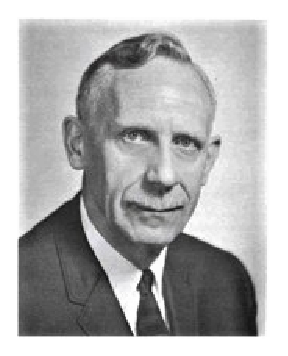
\includegraphics[width=0.9\linewidth]{HendrikBode.eps} 
    \caption*{\index{Bode, Hendrik}\textbf{Hendrik Wade Bode}
    (1905-1982), ingénieur, chercheur et inventeur américain.}
\end{marginfigure}
%-------------------------------------------------------------------------------
L'axe des pulsations étant généralement représenté par une échelle 
logarithmique pour permmettre la représentation de la réponse harmonique sur 
une large plage de valeurs en pulsation (\Cref{annexe-log}). Le calcul de la
phase passe lui par la détermination de l'argument principale 
(\Cref{annexe-NC}).
%-------------------------------------------------------------------------------
\begin{figure}[!h]
    \centering
    \tikzsetnextfilename{sche_bode-chap_repfreq-ext}
    \input{tikz/sche_bode-chap_repfreq.tex}
    \caption{Représentation schématique d'un diagramme de Bode. Le gain en 
             décibel et la phase associé à une fonction de transfert sont 
             représentés en fonction de la pulsation (à l'échelle log) sur 
             deux repères distincts.\label{fig-sche_bode}}
\end{figure}
%-------------------------------------------------------------------------------

La principale propriété du diagramme de Bode est de permettre de 
simplifier un grand nombre calcul. En effet, dans le cas par exemple où 
deux systèmes $H_1$ et $H_2$ sont mis en série,
\[
H(\jw)=H_1(\jw)H_2(\jw),
\]
Le diagramme de Bode de $H(\jw)$ est la somme de deux diagrammes indépendants:
\[
\mathrm{Bode}(total)=\mathrm{Bode}(1)+\mathrm{Bode}(2)
\]
%\newpage
%%%%%%%%%%%%%%%%%%%%%%%%%%%%%%%%%%%%%%%%%%%%%%%%%%%%%%%%%%%%%%%%%%%%%%%%%%%%%%%%
%%%%%%%%%%%%%%%%%%%%%%%%%%%%%%%%%%%%%%%%%%%%%%%%%%%%%%%%%%%%%%%%%%%%%%%%%%%%%%%%
\subsection{Diagramme de Nyquist}
%%%%%%%%%%%%%%%%%%%%%%%%%%%%%%%%%%%%%%%%%%%%%%%%%%%%%%%%%%%%%%%%%%%%%%%%%%%%%%%%
%%%%%%%%%%%%%%%%%%%%%%%%%%%%%%%%%%%%%%%%%%%%%%%%%%%%%%%%%%%%%%%%%%%%%%%%%%%%%%%%
\index{Diagramme! de Nyquist}
%-------------------------------------------------------------------------------
\begin{figure}[!b]
    \centering
    \tikzsetnextfilename{sche_nyquist_1-chap_repfreq-ext}
    \begin{tikzpicture}
\begin{axis}
    [   height=6.5cm,
        width=0.5\linewidth,
        axis lines = center,
        ticks=none,
        axis line style = thick,
        enlargelimits=false,
        xlabel=$\Re{H(\jw)}$,
        ylabel=$\Im{H(\jw)}$,
        xlabel style={below right},
        ylabel style={left},
        ymin=-10,
        ymax=+10,
        xmin=-10,
        xmax=+10
    ]     
    \def\xu{6.65043990901}
    \def\yu{3.24525022405}
    \def\xd{-2.6946926406}
    \def\yd{5.13601319826}
    \addplot[col5, mark = *] coordinates {(0, 0)}  {};
    \node[below] at (axis cs: 7.854, 0)  {\scriptsize$\omega=0$};
    \addplot[col5, mark = *] coordinates {(7.854, 0)} {};
    \node[below] at (axis cs: -2.2, 0)   {\scriptsize$\omega\rightarrow\infty$};
    \addplot[col4, mark = *] coordinates   {(\xu,\yu)} {};
    \node[above right, col4] at (axis cs: \xu,\yu) {\scriptsize$\omega_1$};
    \draw[col4,thick] (axis cs:0,0) -- (axis cs: \xu,\yu) 
    node[midway,yshift=1.1em,xshift=0.6em] {\scriptsize$G(\omega_1)$};
    \draw[col4,thick] (axis cs:2.6,0) arc (0:18:1cm) 
    node[midway,yshift=0.23em,xshift=1.6em] {\scriptsize$\phi(\omega_1)$};
    \addplot[col1, mark = *] coordinates {( \xd,\yd)} {};
    \node[above left, col1]  at (axis cs:  \xd,\yd) {\scriptsize$\omega_2$};
    \draw[col1,thick] (axis cs:0,0) -- (axis cs:\xd,\yd) 
    node[midway,yshift=-0.5em,xshift=-1em] {\scriptsize$G(\omega_2)$};
    \draw[col1,thick] (axis cs:1.9,0) arc (0:119:1.9)    
    node[midway,yshift=-1.7em,xshift=-1.85em] {\scriptsize$\phi(\omega_2)$};
    \addplot[postaction={decorate, decoration={markings,
             mark=at position 0.105 with {\arrow[rotate=-180]{latex};},
             mark=at position 0.31 with  {\arrow[rotate=-180]{latex};},
             mark=at position 0.51 with  {\arrow[rotate=-180]{latex};},
             mark=at position 0.71 with  {\arrow[rotate=-180]{latex};},
             mark=at position 0.9 with   {\arrow[rotate=-180]{latex};}
             }},thick,domain=0:7.853981633974483,samples=100]
             ({x*sin(deg(x))},{x*cos(deg(x))});
\end{axis}
\end{tikzpicture}%

    \tikzsetnextfilename{sche_nyquist_2-chap_repfreq-ext}
    \begin{tikzpicture}
    \begin{axis}
    [   height=6.5cm,
        width=0.45\linewidth,
        axis lines = center,
        ticks=none,
        axis line style = thick,
        enlargelimits=false,
        xlabel=$\Re{H(\jw)}$,
        ylabel=$\Im{H(\jw)}$,
        xlabel style={below right},
        ylabel style={left},
        ymin=-10,
        ymax=+10,
        xmin=-10,
        xmax=+10
    ]     
    \def\xu{6.65043990901}
    \def\yu{3.24525022405}
    \def\xd{-2.6946926406}
    \def\yd{5.13601319826}
    \addplot [postaction={decorate, decoration={markings,
              mark=at position 0.105 with {\arrow[rotate=-180]{latex};},
              mark=at position 0.31 with  {\arrow[rotate=-180]{latex};},
              mark=at position 0.51 with  {\arrow[rotate=-180]{latex};},
              mark=at position 0.71 with  {\arrow[rotate=-180]{latex};},
              mark=at position 0.9 with   {\arrow[rotate=-180]{latex};}
             }},thick,domain=0:7.853981633974483,samples=100]
             ({x*sin(deg(x))},{x*cos(deg(x))});
    \addplot [postaction={decorate, decoration={markings,
              mark=at position 0.105 with {\arrow{latex};},
              mark=at position 0.31 with  {\arrow{latex};},
              mark=at position 0.51 with  {\arrow{latex};},
              mark=at position 0.71 with  {\arrow{latex};},
              mark=at position 0.9 with   {\arrow{latex};}
      }},dashed,thick,domain=0:7.853981633974483,samples=100]
      ({x*sin(deg(x))},{-x*cos(deg(x))});
    \end{axis}
\end{tikzpicture}

    \caption{(gauche) Représentation schématique d'un diagramme de Nyquist. 
             Le nombre complexe $H(\jw)$ est représenté dans le plan 
             complexe pour différentes valeurs de la pulsation $\omega$ de 
             0 à $\infty$. (droite) Représentation schématique du lieu 
             complet de Nyquist, symmétrique par rapport à l'axe des réels.
             \label{fig-sche_nyquist}}
\end{figure}
%-------------------------------------------------------------------------------
%-------------------------------------------------------------------------------
\begin{marginfigure}[2em]
    \centering
    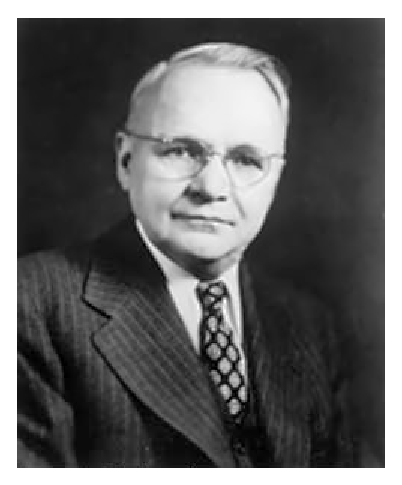
\includegraphics[width=0.9\linewidth]{HarryNyquist} 
    \caption*{\index{Nyquist, Harry}\textbf{Harry Nyquist} (1889-1976), 
              électronicien et ingénieur américain. Il réalisa d'importante 
              contributions à la théorie de l'information.}
\end{marginfigure}
%-------------------------------------------------------------------------------
Un diagramme de Nyquist présente la partie imaginaire et la partie 
réelle de $H(\jw)$ pour différentes 
valeurs paramétrées de $\omega$. Il a l'avantage de combiner les deux 
graphiques du diagramme de Bode en un seul. En effet, la phase et l'amplitude 
d'un point dans le plan complexe peut être déterminé graphiquement par 
respectivement l'angle avec l'axe des réels et la distance à l'origine 
(\Cref{annexe-NC}). Cette représentation graphique est communément appelée 
\textbf{le lieu de Nyquist}. Le lieu de Nyquist complet est le tracé théorique 
des parties réel et imaginaire de $H(\jw)$, en considérant les pulsations 
négatives, c'est à dire entre $\omega\rightarrow-\infty$ et 
$\omega\rightarrow+\infty$.
%\clearpage
%\restoregeometry
%\captionsetup{width=0.9\linewidth}
%%%%%%%%%%%%%%%%%%%%%%%%%%%%%%%%%%%%%%%%%%%%%%%%%%%%%%%%%%%%%%%%%%%%%%%%%%%%%%%%
%%%%%%%%%%%%%%%%%%%%%%%%%%%%%%%%%%%%%%%%%%%%%%%%%%%%%%%%%%%%%%%%%%%%%%%%%%%%%%%%
\subsection{Diagramme de Black-Nichols}
%%%%%%%%%%%%%%%%%%%%%%%%%%%%%%%%%%%%%%%%%%%%%%%%%%%%%%%%%%%%%%%%%%%%%%%%%%%%%%%%
%%%%%%%%%%%%%%%%%%%%%%%%%%%%%%%%%%%%%%%%%%%%%%%%%%%%%%%%%%%%%%%%%%%%%%%%%%%%%%%%
\index{Diagramme! de Black-Nichols}
Le diagramme de Black\footnote{Il également appelé diagramme 
de Black-Nichols ou simplement Nichols dans le monde anglo-saxon.} 
consiste à tracer le gain en décibel $G_{dB}(\omega)$ en fonction de 
la phase, paramétré par la pulsation $\omega$. À l'instar du diagramme de 
Nyquist, le diagramme de Black à l'avantage de combiner les deux graphiques 
du diagramme de Bode. La diagramme de Black est habituellement utilisé dans 
l'étude des systèmes asservis (\Cref{chap-asservis}) pour déterminer le lieu 
de transfert dans le plan de Black d'un système en boucle fermée (FTBF) à 
partir de la connaissance du lieu de transfert dans le plan de Black de la 
Fonction de Transfert en Boucle ouverte (FTBO).
%-------------------------------------------------------------------------------
\begin{marginfigure}
    \centering
    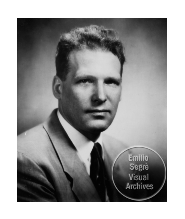
\includegraphics[width=0.9\linewidth]{NathanielNichols.eps} 
    \caption*{\index{Nichols, Nathaniel}\textbf{Nathaniel B. Nichols}, 
              (1914–1997) ingénieur américain.}
\end{marginfigure}
%-------------------------------------------------------------------------------
%(moins important dans une premiere découverte des \SLCI.
%Il pourra être introduit séparément dans le cas des systèmes asservis.)
%-------------------------------------------------------------------------------
\begin{figure}[!h]
    \centering
    \tikzsetnextfilename{sche_black-chap_repfreq-ext}
    \begin{tikzpicture}
\begin{axis}
    [
    clip=false,
    height=8cm,
    width=8cm,
    ticks=none,
    axis lines = center,
    axis line style = thick,
    enlargelimits=false,
    ylabel=$G(\omega)$,
    xlabel=$\phi(\omega)$,
    xlabel style={right},
    ylabel style={above},
    xticklabel style={above,yshift=0.3em},
    yticklabel style={right,xshift=0.3em},
    ymin=-60,
    ymax=+10,
    xmin=-100,
    xmax=+20
    ]     
    \addplot[thick,domain=0:10,samples=100] 
    ({-atan2(x,1)},{-10*log10(1+x*x)});
    \addplot[thick,domain=10:100,samples=100,-latex] 
    ({-atan2(x,1)},{-10*log10(1+x*x)});
    \addplot[thick,domain=100:1000,samples=100] 
    ({-atan2(x,1)},{-10*log10(1+x*x)});
    \addplot[col5, mark = *] coordinates {(0,0)} {};                    
    \addplot[col5, mark = *,col1] coordinates 
    {({-atan2(10,1)},{-10*log10(1+10*10)} )} {};                    
    \draw[thick,col1,dashed] (axis cs: {-atan2(10,1)},{-10*log10(1+10*10)}) --
    (axis cs: {-atan2(10,1)},0) node[above] {$\phi(\omega_2)$};
    \draw[thick,col1,dashed] (axis cs: {-atan2(10,1)},{-10*log10(1+10*10)}) --
    (axis cs: 0,{-10*log10(1+10*10)}) node[right] {$G_{dB}(\omega_2)$};
    \addplot [col5, mark = *,col4] coordinates 
    {({-atan2(2,1)},{-10*log10(1+4)} )} {};
    \draw[thick,col4,dashed] (axis cs: {-atan2(2,1)},{-10*log10(5)}) -- 
                            (axis cs: {-atan2(2,1)},0) 
                            node[above] {$\phi(\omega_1)$};
    \draw[thick,col4,dashed] (axis cs: {-atan2(2,1)},{-10*log10(5)}) --
                             (axis cs: 0,{-10*log10(5)}) 
                            node[right] {$G_{dB}(\omega_1)$};
    \node [above right]  at (axis cs: 0 , 0)   {$\omega=0$}; 
    \node [above right]  at (axis cs:-90, -60) {$\omega\rightarrow+\infty$}; 

\end{axis}
\end{tikzpicture}

    \caption{Représentation schématique d'un diagramme de Black. Le gain et 
             la phase de la fonction de transfert $H(\jw)$ sont représentés sur
             le lieu de Black pour différentes valeurs de la pulsation $\omega$
             de 0 à $\infty$.\label{fig-sche_black}}
\end{figure}
%-------------------------------------------------------------------------------
\newpage
\restoregeometry
\captionsetup{width=0.9\linewidth}
%%%%%%%%%%%%%%%%%%%%%%%%%%%%%%%%%%%%%%%%%%%%%%%%%%%%%%%%%%%%%%%%%%%%%%%%%%%%%%%%
%%%%%%%%%%%%%%%%%%%%%%%%%%%%%%%%%%%%%%%%%%%%%%%%%%%%%%%%%%%%%%%%%%%%%%%%%%%%%%%%
%%%%%%%%%%%%%%%%%%%%%%%%%%%%%%%%%%%%%%%%%%%%%%%%%%%%%%%%%%%%%%%%%%%%%%%%%%%%%%%%
\section{Analyse fréquentielle des modèles usuels}
%%%%%%%%%%%%%%%%%%%%%%%%%%%%%%%%%%%%%%%%%%%%%%%%%%%%%%%%%%%%%%%%%%%%%%%%%%%%%%%%
%%%%%%%%%%%%%%%%%%%%%%%%%%%%%%%%%%%%%%%%%%%%%%%%%%%%%%%%%%%%%%%%%%%%%%%%%%%%%%%%
%%%%%%%%%%%%%%%%%%%%%%%%%%%%%%%%%%%%%%%%%%%%%%%%%%%%%%%%%%%%%%%%%%%%%%%%%%%%%%%%
Nous allons ici présenter la forme canonique des diagrammes fréquentielles 
(Bode, Nyquist et Black-Nichols) pour les modèles usuels rencontrées dans 
l'étude des \gls{slci}. Les diagrammes de Bode restent l'outil principale et 
fera l'objet d'une présentation plus détaillée.
%%%%%%%%%%%%%%%%%%%%%%%%%%%%%%%%%%%%%%%%%%%%%%%%%%%%%%%%%%%%%%%%%%%%%%%%%%%%%%%%
%%%%%%%%%%%%%%%%%%%%%%%%%%%%%%%%%%%%%%%%%%%%%%%%%%%%%%%%%%%%%%%%%%%%%%%%%%%%%%%%
\subsection{Diagrammes de Bode : méthodologie générale}
%%%%%%%%%%%%%%%%%%%%%%%%%%%%%%%%%%%%%%%%%%%%%%%%%%%%%%%%%%%%%%%%%%%%%%%%%%%%%%%%
%%%%%%%%%%%%%%%%%%%%%%%%%%%%%%%%%%%%%%%%%%%%%%%%%%%%%%%%%%%%%%%%%%%%%%%%%%%%%%%%
Pour chacun des modèles usuels, à savoir : un gain pur, un intégrateur pur,
un dérivateur pur, un retard pur, un système du premier ordre et du second 
ordre, nous allons déterminer les diagrammes de Bode dits asymptotiques 
et réels. Le diagramme réel est la représentation exacte des fonctions du gain
en décibel et de la phase en fonction de la pulsation d'entrée de 
la sollicitation. Le diagramme asymptotique permet de caractériser 
qualitativement l'effet du modèle usuel sur le diagramme de Bode. 
Dans la pratique, on ne s'interresse qu'aux limites aux basses et hautes 
fréquences. Nous pourrons vérifier que cette approximation asymptotiques est une
approximation pour la fonction du gain.

Pour résumer, nous appliquerons la procédure suivante à chacun des modèles 
usuels :
%-------------------------------------------------------------------------------
\begin{itemize}
    \item[i)] Définir la fonction de transfert complexe $H(\jw)$ à partir de la 
          fonction de transfert $H(p)$ du modèle en question pour $p=\jw$.
    \item[ii)] \'Etablir la fonction du gain $G(\omega)$ à partir du 
          module de $H(\jw)$.
    \item[iii)] Déterminer le gain en décibel $G_{\si{\dB}}$ tel que 
        $G_{\si{\dB}}=20\log{G(\omega)}$.
    \item[iv)] \'Etablir la fonction de la phase $\phi(\omega)$ à partir de 
        l'argument principale de $H(\jw)$.
        \footnote{L'argument principale est l'argument d'un nombre complexe 
        dans $[-\pi,\pi]$. On se raportera à l'\Cref{annexe-NC} pour plus 
        de détails.}
    \item[v)] Si les fonctions $G(\omega)$ et $\phi(\omega)$ ne sont pas de 
          simples constantes, réalisér une étude
          asymptotique pour $\omega\rightarrow 0$ et 
          $\omega\rightarrow +\infty$.
    \item[vi)] Tracer le diagramme de Bode \textbf{réel} et le diagramme 
          de Bode \textbf{asymptotique} sur un graphe semi-logarithmique.
\end{itemize}
%-------------------------------------------------------------------------------
\newpage
%%%%%%%%%%%%%%%%%%%%%%%%%%%%%%%%%%%%%%%%%%%%%%%%%%%%%%%%%%%%%%%%%%%%%%%%%%%%%%%%
\subsubsection{Diagramme de Bode d'un gain pur}
%%%%%%%%%%%%%%%%%%%%%%%%%%%%%%%%%%%%%%%%%%%%%%%%%%%%%%%%%%%%%%%%%%%%%%%%%%%%%%%%
\index{Gain pur!diagramme de Bode}
La fonction de transfert d'un gain pur est de la forme $H(\jw)=K$,
le gain est donc simplement donné par 
\[
G(\omega)=|H(\jw)|=K.
\] 
D'où le gain $G_{dB}$ en décibel :
%-------------------------------------------------------------------------------
\begin{bequation}[ams align*]
G_{dB}(\omega)= 20\log{K}
\end{bequation} 
%-------------------------------------------------------------------------------
ce qui correspond à une constante pour un gain statique $K$ 
donné (\Cref{fig-bode_gain})
En ce qui concerne la phase, elle s'obtient à partir de l'argument 
principale du nombre complexe $H(\jw)$:
%-------------------------------------------------------------------------------
\begin{bequation}[ams align*]
\phi(\omega) = 0
\end{bequation}
%-------------------------------------------------------------------------------
Un gain pur n'a donc aucun effet sur le déphasage quelque soit la pulsation
d'entrée.
%-------------------------------------------------------------------------------
\begin{figure}[!h]
    \centering
    \tikzsetnextfilename{bode_gain_1-chap_repfreq-ext}
    \input{tikz/bode_gain_1-chap_repfreq.tex}

    \tikzsetnextfilename{bode_gain_2-chap_repfreq-ext}
    \begin{tikzpicture}[trim axis left]
\begin{axis}[
    ticklabel style = {font=\footnotesize},
    width=0.9\textwidth,
    height=0.25\textheight,
    xlabel={Pulsation (\si{\radian\per\second})},
    ylabel={Phase (deg)},
    xtick={1e-3,1e-2,1e-1,1,1e1,1e2,1e3}, 
    ytick={-90,-45,0,45,90}, 
    yticklabels={-90,-45,0,45,90},
    xticklabels={$10^{-3}$,$10^{-2}$,$10^{-1}$,
                 $10^{0}$,$10^{1}$,$10^{2}$,$10^{3}$},
    xmode=log,ymode=normal,
    xmin=1e-3, xmax=1e3,
    ymin=-90, ymax=90,
    grid=both,
    major grid style={black!40}
]
    \addplot[ultra thick, col1,domain=1e-3:1e3, samples=101] {0}; 
\end{axis}
\end{tikzpicture}

    \caption{Diagramme de Bode d'un gain pur avec (noir) 
             $K=0.1$, (bleu) $K=1$ et (rouge) $K=10$. Remarquons que la 
             phase reste inchangée lorsque le gain statique $K$ varie et que 
             seul le gain $G_{dB}(\omega)$ est modifié. \label{fig-bode_gain}}
\end{figure}
%-------------------------------------------------------------------------------
\newpage
%%%%%%%%%%%%%%%%%%%%%%%%%%%%%%%%%%%%%%%%%%%%%%%%%%%%%%%%%%%%%%%%%%%%%%%%%%%%%%%%
\subsubsection{Diagramme de Bode d'un intégrateur pur}
%%%%%%%%%%%%%%%%%%%%%%%%%%%%%%%%%%%%%%%%%%%%%%%%%%%%%%%%%%%%%%%%%%%%%%%%%%%%%%%%
\index{Intégrateur pur!diagramme de Bode}
La fonction de transfert d'un intégrateur pur est de la forme 
$H(\jw)=\frac{K}{\jw}$, le gain est donc simplement donné par 
\[
G(\omega)=|H(\jw)|=\frac{K}{\omega},
\] 
d'où le gain $G_{dB}$ en décibel :
%-------------------------------------------------------------------------------
\begin{bequation}[ams align*]
G_{dB}(\omega)= 20\log{K} - 20\log{\omega}
\end{bequation} 
%-------------------------------------------------------------------------------
ce qui correspond à une pente de \SI{-20}{\dB\per\dec} (\Cref{fig-bode_int}).
La phase s'obtient à partir de l'argument principale 
du nombre complexe $H(\jw)$:
%-------------------------------------------------------------------------------
\begin{bequation}[ams align*]
\phi(\omega) = -\dfrac{\pi}{2}
\end{bequation}
%-------------------------------------------------------------------------------
Un intégrateur pur déphase donc la sortie de -90\degree~quelque soit la 
pulsation de l'entrée.
%-------------------------------------------------------------------------------
\begin{figure}[!htb]
    \centering
    \tikzsetnextfilename{bode_integ_1-chap_repfreq-ext}
    \input{tikz/bode_integ_1-chap_repfreq.tex}

    \tikzsetnextfilename{bode_integ_2-chap_repfreq-ext}
    \input{tikz/bode_integ_2-chap_repfreq.tex}
    \caption{Diagramme de Bode d'un intégrateur pur avec (noir) 
             $K=0.1$, (bleu) $K=1$ et (rouge) $K=10$. Remarquons 
             que le gain s'annule pour $\omega=K$ et que la phase reste 
             inchangée.\label{fig-bode_int}}
\end{figure}
%-------------------------------------------------------------------------------
\newpage
%%%%%%%%%%%%%%%%%%%%%%%%%%%%%%%%%%%%%%%%%%%%%%%%%%%%%%%%%%%%%%%%%%%%%%%%%%%%%%%%
\subsubsection{Diagramme de Bode d'un dérivateur pur}
%%%%%%%%%%%%%%%%%%%%%%%%%%%%%%%%%%%%%%%%%%%%%%%%%%%%%%%%%%%%%%%%%%%%%%%%%%%%%%%%
\index{Dérivateur pur!diagramme de Bode}
La fonction de transfert d'un dérivateur pur est de la forme $H(\jw)=K\jw$,
le gain est donc simplement donné par 
\[
G(\omega)=|H(\jw)|=K\jw
\] 
d'où le gain $G_{dB}$ en décibel :
%-------------------------------------------------------------------------------
\begin{bequation}[ams align*]
    G_{dB}(\omega)= 20\log{K} + 20\log{\omega}
\end{bequation}
%-------------------------------------------------------------------------------
ce qui correspond à une pente de \SI{+20}{\dB\per\dec} (\Cref{fig-bode_deriv}).
La phase s'obtient simplement par l'argument principal de $H(\jw)$:
%-------------------------------------------------------------------------------
\begin{bequation}[ams align*]
    \phi(\omega) = \dfrac{\pi}{2}
\end{bequation}
%-------------------------------------------------------------------------------
Un dérivateur pur déphase la sortie de +90\degree~quelque soit la pulsation 
d'entrée.
%-------------------------------------------------------------------------------
\begin{figure}[!htb]
    \centering
    \tikzsetnextfilename{bode_deriv_1-chap_repfreq-ext}
    \begin{tikzpicture}[trim axis left]
\begin{axis}[
    ticklabel style = {font=\footnotesize},
    width=0.9\textwidth,
    height=0.25\textheight,
    ylabel={Gain (dB)},
    xtick={1e-3,1e-2,1e-1,1,1e1,1e2,1e3}, 
    ytick={-60,-40,-20,0,20,40,60}, 
    xticklabels={$10^{-3}$,$10^{-2}$,$10^{-1}$,
                 $10^{0}$,$10^{1}$,$10^{2}$,$10^{3}$},
    yticklabels={-60,-40,-20,0,20,40,60}, 
    xmode=log,ymode=normal,
    xmin=1e-3, xmax=1e3,
    ymin=-60, ymax=60,
    grid=both,
    major grid style={black!40}
]
    \addplot[ultra thick,col5,domain=1e-3:1e3, samples=101]
    {20*log10(0.1)+20*log10(x)}; 
    \addplot[ultra thick, col1,domain=1e-3:1e3, samples=101] {20*log10(x)};
    \addplot[ultra thick, col4,domain=1e-3:1e3, samples=101] 
    {20*log10(10)+20*log10(x)};
\end{axis}
\end{tikzpicture}


    \tikzsetnextfilename{bode_deriv_2-chap_repfreq-ext}
    \begin{tikzpicture}[trim axis left]
\begin{axis}[
    ticklabel style = {font=\footnotesize},
    width=0.9\textwidth,
    height=0.25\textheight,
    xlabel={Pulsation (rad/s)},
    ylabel={Phase (deg)},
    xtick={1e-3,1e-2,1e-1,1,1e1,1e2,1e3}, 
    ytick={0,45,90,135,180}, 
    yticklabels={0,45,90,135,180}, 
    xticklabels={$10^{-3}$,$10^{-2}$,$10^{-1}$,
                 $10^{0}$,$10^{1}$,$10^{2}$,$10^{3}$},
    xmode=log,ymode=normal,
    xmin=1e-3, xmax=1e3,
    ymin=0, ymax=180,
    grid=both,
    major grid style={black!40}
]
    \addplot[ultra thick, col1,domain=1e-3:1e3, samples=101] {atan(1000000)};
\end{axis}
\end{tikzpicture}

    \caption{Diagramme de Bode d'un dérivateur pur 
             avec (noir) $K=0.1$, (bleu) $K=1$ et (rouge) $K=10$. Remarquons 
             que le gain s'annule pour $\omega=\frac{1}{K}$ et que la phase 
             reste inchangée.\label{fig-bode_deriv}}
\end{figure}
%-------------------------------------------------------------------------------
\newpage
%%%%%%%%%%%%%%%%%%%%%%%%%%%%%%%%%%%%%%%%%%%%%%%%%%%%%%%%%%%%%%%%%%%%%%%%%%%%%%%%
\subsubsection{Diagramme de Bode d'un système à retard pur}
%%%%%%%%%%%%%%%%%%%%%%%%%%%%%%%%%%%%%%%%%%%%%%%%%%%%%%%%%%%%%%%%%%%%%%%%%%%%%%%%
\index{Retard pur!diagramme de Bode}
La fonction de transfert d'un retard pur est de la forme $H(\jw)=e^{-\jtw}$,
le gain est donc simplement donné par
\[
G(\omega)=|H(\jw)|=1
\]
d'où le gain $G_{dB}$ en décibel :
%-------------------------------------------------------------------------------
\begin{bequation}[ams align*]
    G_{dB}(\omega)= \SI{0}{\decibel}
\end{bequation}
%-------------------------------------------------------------------------------
ce qui correspond à un gain constant (\Cref{fig-bode_retard_1}).
La phase s'écrit simplement à partir de l'argument principal de $H(\jw)$ :
%-------------------------------------------------------------------------------
\begin{bequation}[ams align*]
    \phi(\omega) = -\tau\omega
\end{bequation}
%-------------------------------------------------------------------------------
Le déphasage d'un retard pur croit linéairement avec la pulsation pour un 
retard de temps $\tau$ donné.
%-------------------------------------------------------------------------------
\begin{figure}[!htb]
    \centering
    \tikzsetnextfilename{bode_retard_1-chap_repfreq-ext}
    \input{tikz/bode_retard_1-chap_repfreq.tex}

    \tikzsetnextfilename{bode_retard_2-chap_repfreq-ext}
    \input{tikz/bode_retard_2-chap_repfreq.tex}
    \caption{Diagramme de Bode d'un retard pur 
             avec $\tau=1$. Remarquons que le gain est constant pour toutes 
             pulsations et le déphasage est monotone décroissant en fonction 
             de la pulsation\label{fig-bode_retard_1}.}
\end{figure}
%-------------------------------------------------------------------------------
\newpage
%%%%%%%%%%%%%%%%%%%%%%%%%%%%%%%%%%%%%%%%%%%%%%%%%%%%%%%%%%%%%%%%%%%%%%%%%%%%%%%%
\subsubsection{Diagramme de Bode d'un système du premier ordre}
%%%%%%%%%%%%%%%%%%%%%%%%%%%%%%%%%%%%%%%%%%%%%%%%%%%%%%%%%%%%%%%%%%%%%%%%%%%%%%%%
\index{Système du premier ordre!diagramme de Bode}
Un système du premier ordre présente une fonction de transfert de la forme:
%-------------------------------------------------------------------------------
\begin{align}
H(\jw)=\dfrac{K}{1+j\tau\omega }\label{eq-1er_ftjw}
\end{align}
%-------------------------------------------------------------------------------
Le module de cette fonction de transfert $G(\omega) =|H(\jw)|$ s'écrit :
\[
    G(\omega)=\dfrac{K}{\sqrt{1+\tau^2\omega^2}}
\]
Le gain en dB s'obtient alors par :
%-------------------------------------------------------------------------------
\begin{bequation}[ams align]
    G_{dB}(\omega)=20\log{K}-20\log{\sqrt{1+\tau^2\omega^2}}\label{eq-gain_1er}
\end{bequation}
%-------------------------------------------------------------------------------
et la phase est simplement donné par la fonction tangente réciproque:
%-------------------------------------------------------------------------------
\begin{bequation}[ams align]
    \phi(\omega)=\arg{H(\jw)}=-\arctan{(\tau\omega)}\label{eq-phase_1er} 
\end{bequation}
%-------------------------------------------------------------------------------
Ce sont ces deux fonctions de la fréquence que nous traçons sur un diagramme
de Bode. Elles sont représentés sur les~\cref{fig-bode_1er_1,fig-bode_1er_2}, 
pour respectivement différentes valeurs du gain statique $K$ et du temps 
caractéristique $\tau$.
\newline
Il est cependant recommandé de déterminer les asymptotes 
de ces deux fonctions à basse et haute fréquence. 
Pour celà, nous introduisons une \textbf{fréquence de cassure} 
$\omega_c=\dfrac{1}{\tau}$ qui délimite ces deux domaines.
\`A cette fréquence, le gain en décibel est de $G_{dB}(\omega_c)=20\log{K}-3$ 
et la phase $\phi(\omega)=\arctan{(1)}=\dfrac{\pi}{4}$.
Le gain de -3dB est la valeur approximative de $20\log{\sqrt{2}}$, communément
utilisée pour définir la \textbf{fréquence de coupure}.

\`A basse fréquence, c'est à dire lorsque $\tau\omega\ll1$ ou 
encore $\omega\ll\omega_0$, le gain et la phase se comporte comme, 
%-------------------------------------------------------------------------------
\begin{bequation}[ams align*]
    G_{dB}(\omega)&\sim20\log{K} \\
    \phi(\omega)&\sim0\si{\degree}.
\end{bequation} 
%-------------------------------------------------------------------------------
\`A haute fréquence, c'est à dire lorsque $\tau\omega\gg1$ ou 
encore $\omega\gg\omega_0$, le gain et la phase se comporte comme,
%-------------------------------------------------------------------------------
\begin{bequation}[ams align*]
    G_{dB}(\omega)&\sim20\log{K}-20\log{\frac{\omega}{\omega_0}} \\
    \phi(\omega)&\sim-\dfrac{\pi}{2}.
\end{bequation} 
%-------------------------------------------------------------------------------
La~\cref{fig-bode_1er_3} présente sur un même diagramme de Bode, les courbes 
réels et les courbes asymptotiques.
%-------------------------------------------------------------------------------
\begin{figure}[!t]
    \centering
    \tikzsetnextfilename{bode_1er_1-chap_repfreq-ext}
    \input{tikz/bode_1er_1-chap_repfreq.tex}

    \tikzsetnextfilename{bode_1er_2-chap_repfreq-ext}
    \input{tikz/bode_1er_2-chap_repfreq.tex}
    \caption{Diagramme de Bode d'un système du premier ordre 
             (\Cref{eq-1er_ftjw}) avec (noir) $K=0.1$ (bleu) $K=1$ et 
             (rouge) $K=10$. L'effet du gain $K$ est de décaler verticalement 
             la courbe de gain.\label{fig-bode_1er_1}}
\end{figure}
%-------------------------------------------------------------------------------
%-------------------------------------------------------------------------------
\begin{figure}[!b]
    \centering
    \tikzsetnextfilename{bode_1er_3-chap_repfreq-ext}
    \input{tikz/bode_1er_3-chap_repfreq.tex}

    \tikzsetnextfilename{bode_1er_4-chap_repfreq-ext}
    \input{tikz/bode_1er_4-chap_repfreq.tex}
    \caption{Diagramme de Bode d'un système du premier ordre 
             (\Cref{eq-1er_ftjw}) avec (noir) $\tau=10$ (bleu) $\tau=1$ et 
             (rouge) $\tau=0.1$. L'effet du temps caractéristique $\tau$ est 
             de décaler horizontalement la courbe de phase.
             \label{fig-bode_1er_2}}
\end{figure}
%-------------------------------------------------------------------------------
\afterpage{\clearpage}
%-------------------------------------------------------------------------------
\begin{figure}[!t]
\centering
\tikzsetnextfilename{bode_1er_5-chap_repfreq-ext}
\begin{tikzpicture}[trim axis left]
\begin{axis}[
    ticklabel style = {font=\footnotesize},
    width=0.9\textwidth,
    height=0.22\textheight,
    ylabel={Gain (dB)},
    xtick={1e-1,1,1e1}, 
    ytick={-10,-8,-6,-4,-2,0,2}, 
    xticklabels={$10^{-1}$,$10^{0}$,$10^{1}$},
    yticklabels={-10,-8,-6,-4,-2,0,2}, 
    xmode=log,ymode=normal,
    xmin=1e-1, xmax=1e1,
    ymin=-10, ymax=3,
    grid=both,
    major grid style={black!40}
]
    \addplot[ultra thick,col1,domain=1e-3:1e3, samples=101] 
    {-20*log10(sqrt(1+x*x))};
    \addplot[line width=2pt,col4,dashed,domain=1e-1:1e0, samples=101] {0};
    \addplot[line width=2pt,col4,dashed,domain=1e0:1e1, samples=101] 
    {-20*log10(x)};
\end{axis}
\end{tikzpicture}


\tikzsetnextfilename{bode_1er_6-chap_repfreq-ext}
\begin{tikzpicture}[trim axis left]
\begin{axis}[
    ticklabel style = {font=\footnotesize},
    width=0.9\textwidth,
    height=0.22\textheight,
    xlabel={Pulsation (rad/s)},
    ylabel={Phase (deg)},
    xtick={1e-1,1,1e1}, 
    ytick={-90,-45,0}, 
    yticklabels={-90,-45,0},
    xticklabels={$10^{-1}$,$10^{0}$,$10^{1}$},
    xmode=log,ymode=normal,
    xmin=1e-1, xmax=1e1,
    ymin=-90, ymax=0,
    grid=both,
    major grid style={black!40}
]
    \addplot[ultra thick,col1,domain=1e-3:1e3, samples=101] {-atan2(x,1)};
    \addplot[line width=2pt,col4,dashed,domain=1e-1:1e0,samples=101] {0};
    \addplot[line width=2pt,col4,dashed,domain=1e0:1e1,samples=101] {-90};
    \draw[line width=2pt,col4,dashed] (axis cs:1,0) -- (axis cs:1,-90);
\end{axis}
\end{tikzpicture}

\caption{Diagramme de Bode d'un système du premier ordre 
         (\Cref{eq-1er_ftjw}) (c.-à-d. $K=1$, $\tau=1$ et $\omega_c=1$) avec 
         (bleu) le diagramme réel et (rouge) le diagramme asymptotique. On 
         vérifie que les valeurs asymptotiques sont de bonnes approximations 
         à basse et haute fréquence. Il est également possible de lire un 
         gain de \SI{-3}{\dB} et une phase de -45\si{\degree} à la fréquence 
         de coupure.\label{fig-bode_1er_3}}
\end{figure}
%-------------------------------------------------------------------------------
%%%%%%%%%%%%%%%%%%%%%%%%%%%%%%%%%%%%%%%%%%%%%%%%%%%%%%%%%%%%%%%%%%%%%%%%%%%%%%%%
\subsubsection{Diagramme de Bode de deux systèmes du premier ordre en série }
%%%%%%%%%%%%%%%%%%%%%%%%%%%%%%%%%%%%%%%%%%%%%%%%%%%%%%%%%%%%%%%%%%%%%%%%%%%%%%%%
La fonction de transfert globale de deux systèmes du premier ordre en série 
s'écrit:
%-------------------------------------------------------------------------------
\begin{align}
    H(\jw)=\dfrac{K_1K_2}{(1+j\tau_1\omega)(1+j\tau_2\omega)}
    \label{eq-1er_serie}
\end{align}
%-------------------------------------------------------------------------------
On utilise la propriété du logarithme pour écrire le gain globale 
$G_{dB}(\omega)$ comme une somme de gain de deux systèmes du premier ordre, 
soit
\[
G_{dB}(\omega) = G_{dB1}(\omega) + G_{dB2}(\omega)
\]
De même pour la phase:
\[
\phi(\omega)= \phi_1(\omega) + \phi_2(\omega)
\]
En reprenant les~\cref{eq-gain_1er,eq-phase_1er} on établit facilement que,
%-------------------------------------------------------------------------------
\begin{bequation}[ams align*]
    G_{dB}(\omega) = 20\log{K_1K_2}-20\log{\sqrt{1+\tau_1^2\omega^2}}
                    -20\log{\sqrt{1+\tau_2^2\omega^2}}
\end{bequation}
%-------------------------------------------------------------------------------
et
%-------------------------------------------------------------------------------
\begin{bequation}[ams align*]
    \phi(\omega)=-\arctan{\tau_1\omega}-\arctan{\tau_2\omega}
\end{bequation}
%-------------------------------------------------------------------------------
L'étude asymptotique se fait en considérant deux fréquences de coupures 
$\omega_{c1}=\frac{1}{\tau_1}$ et $\omega_{c2}=\frac{1}{\tau_2}$.
Supposons d'abord, sans perte de généralité, que $\omega_{c2}>\omega_{c1}$ et 
considérons 
les trois domaines de fréquence ainsi définits selon que 
$\omega\ll\omega_{c1}$, $\omega_{c1}<\omega<\omega_{c1}$ ou 
$\omega\gg\omega_{c2}$
%%%%%%%%%%%%%%%%%%%%%%%%%%%%%%%%%%%%%%%%%%%%%%%%%%%%%%%%%%%%%%%%%%%%%%%%%%%%%%%%
\paragraph{Pour $\omega\ll\omega_{c1}$}
%%%%%%%%%%%%%%%%%%%%%%%%%%%%%%%%%%%%%%%%%%%%%%%%%%%%%%%%%%%%%%%%%%%%%%%%%%%%%%%%
%-------------------------------------------------------------------------------
\begin{bequation}[ams align*]
    G_{dB}(\omega)&\sim20\log{K_1K_2}\\
      \phi(\omega)&\sim0\si{\degree}
\end{bequation}
%-------------------------------------------------------------------------------
%%%%%%%%%%%%%%%%%%%%%%%%%%%%%%%%%%%%%%%%%%%%%%%%%%%%%%%%%%%%%%%%%%%%%%%%%%%%%%%%
\paragraph{Pour $\omega_{c1}<\omega<\omega_{c1}$}
%%%%%%%%%%%%%%%%%%%%%%%%%%%%%%%%%%%%%%%%%%%%%%%%%%%%%%%%%%%%%%%%%%%%%%%%%%%%%%%%
%-------------------------------------------------------------------------------
\begin{bequation}[ams align*]
    G_{dB}(\omega)&\sim20\log{K_1K_2}-20\log{\dfrac{\omega}
                                        {\omega_{c1}\omega_{c2}}}\\
    \phi(\omega)&\sim-90\si{\degree}
\end{bequation}
%-------------------------------------------------------------------------------
%%%%%%%%%%%%%%%%%%%%%%%%%%%%%%%%%%%%%%%%%%%%%%%%%%%%%%%%%%%%%%%%%%%%%%%%%%%%%%%%
\paragraph{Pour $\omega\gg\omega_{c2}$}
%%%%%%%%%%%%%%%%%%%%%%%%%%%%%%%%%%%%%%%%%%%%%%%%%%%%%%%%%%%%%%%%%%%%%%%%%%%%%%%%
%-------------------------------------------------------------------------------
\begin{bequation}[ams align*]
    G_{dB}(\omega)&\sim20\log{K_1K_2}-40\log{\dfrac{\omega}
                                        {\omega_{c1}\omega_{c2}}}\\
    \phi(\omega)&\sim-180\si{\degree}
\end{bequation}
%-------------------------------------------------------------------------------
La~\cref{fig-bode_1er_serie} présente le diagramme de Bode réel et 
asymptotique de deux systèmes du premier ordre en cascade. On remarquera 
que l'approximation asymptotique est suffisante pour décrire le gain de ce 
genre de système. En marquant la discontinuité dans le graphe de la phase, 
on distingue plus facilement les différentes zones et les changements de 
pente du gain. Pour la phase, il suffit de déterminer sa valeur pour 
quelques valeurs particulières de la pulsation. 

Comme nous l'avons déjà rencontré, l'étude de deux systèmes du premier 
ordre en série correspond à l'étude d'un système du second ordre en 
régime apériodique.
%-------------------------------------------------------------------------------
\begin{figure}[!t]
    \centering
    \tikzsetnextfilename{bode_1er_serie_2nd_1-chap_repfreq-ext}
    \begin{tikzpicture}[trim axis left]
\begin{axis}[
    ticklabel style = {font=\footnotesize},
    width=0.9\textwidth,
    height=0.25\textheight,
    ylabel={Gain (dB)},
    xtick={1e-3,1e-2,1e-1,1,1e1,1e2,1e3}, 
    ytick={-80,-60,-40,-20,0,20,40,60}, 
    xticklabels={$10^{-3}$,$10^{-2}$,$10^{-1}$,
                 $10^{0}$,$10^{1}$,$10^{2}$,$10^{3}$},
    yticklabels={-80,-60,-40,-20,0,20,40,60}, 
    xmode=log,ymode=normal,
    xmin=1e-3, xmax=1e3,
    ymin=-120, ymax=20,
    grid=both,
    major grid style={black!40}
]
    \addplot[ultra thick, col1,domain=1e-3:1e3, samples=101]
    {-20*log10(sqrt(1+100*x*x))-20*log10(sqrt(1+0.01*x*x))}; 
    \addplot[line width=2pt,col4,dashed,domain=1e-3:1e-1, samples=101]{0};
    \addplot[line width=2pt,col4,dashed,domain=1e-1:1e1, samples=101]
    {-20*log10(x/0.1)};
    \addplot[line width=2pt,col4,dashed,domain=1e1:1e3, samples=101]
    {-20*log10(x/0.1)-20*log10(x/10)};
    \node[right,xshift=1em,yshift=-0.1em] at (axis cs:0.1,-70)
    {{\large \textbf{-20dB/décade}}};
    \node[right,xshift=1em,yshift=-0.1em] at (axis cs:10,-10)
    {{\large \textbf{-40dB/décade}}};
\end{axis}
\end{tikzpicture}


    \tikzsetnextfilename{bode_1er_serie_2nd_2-chap_repfreq-ext}
    \input{tikz/bode_1er_serie_2nd_2-chap_repfreq.tex}
    \caption{Diagramme de Bode de systèmes du premier ordre en série 
    (\Cref{eq-1er_serie}) avec $\tau_1=10$ et $\tau_2=0.1$ (bleu) le 
    diagramme réel et (rouge) le diagramme asymptotique.
    \label{fig-bode_1er_serie}}
\end{figure}
%-------------------------------------------------------------------------------
%\newpage
%%%%%%%%%%%%%%%%%%%%%%%%%%%%%%%%%%%%%%%%%%%%%%%%%%%%%%%%%%%%%%%%%%%%%%%%%%%%%%%%
\subsubsection{Diagramme de Bode d'un système second d'ordre}
%%%%%%%%%%%%%%%%%%%%%%%%%%%%%%%%%%%%%%%%%%%%%%%%%%%%%%%%%%%%%%%%%%%%%%%%%%%%%%%%
\index{Système du second ordre!diagramme de Bode}
La fonction de transfert d'un système du second ordre (\Cref{eq-2nd_ft}) 
est donnée par :
%-------------------------------------------------------------------------------
\begin{align}
    H(\jw)=\dfrac{K\omega^2_0}{(\omega^2_0-\omega^2)+j2\xi\omega_0\omega}
    \label{eq-2nd_ftjw}
\end{align}
%-------------------------------------------------------------------------------
Le gain s'obtient en calculant le module de ce nombre complexe :
\[
    G(\omega)=\dfrac{K\omega^2_0}{\sqrt{(\omega^2_0-\omega^2)^2
         +(2\xi\omega_0\omega)^2}}
\]
Le gain en décibel s'écrit alors :
%-------------------------------------------------------------------------------
\begin{bequation}[ams align*]
    G_{db}(\omega)=20\log{K\omega_0^2}-20\log{\sqrt{(\omega^2_0-\omega^2)^2
                                               +(2\xi\omega_0\omega)^2}}
\end{bequation}
%-------------------------------------------------------------------------------
et la phase par l'argument princiale:
%-------------------------------------------------------------------------------
\begin{bequation}[ams align*]
    \phi(\omega)=
    \begin{cases}
    -\arctan{\left(\dfrac{2\xi\omega_0\omega}{\omega_0^2-\omega^2}\right)}     
        &\,\,\,\,\text{si $\omega^2<\omega^2_0$}\\
    -\arctan{\left(\dfrac{2\xi\omega_0\omega}{\omega_0^2-\omega^2}\right)}+\pi 
        &\,\,\,\,\text{si $\omega^2>\omega^2_0$}\\
    -\dfrac{\pi}{2}                                                            
    &\,\,\,\,\text{si $\omega^2=\omega^2_0$}
    \end{cases}
\end{bequation}
%-------------------------------------------------------------------------------
Comme précédemment, il est recommandé d'étudier les valeurs asymptotiques 
du gain et de la phase.
%%%%%%%%%%%%%%%%%%%%%%%%%%%%%%%%%%%%%%%%%%%%%%%%%%%%%%%%%%%%%%%%%%%%%%%%%%%%%%%%
\paragraph{Pour $\omega \ll\omega_0$}
%%%%%%%%%%%%%%%%%%%%%%%%%%%%%%%%%%%%%%%%%%%%%%%%%%%%%%%%%%%%%%%%%%%%%%%%%%%%%%%%
%-------------------------------------------------------------------------------
\begin{bequation}[ams align*]
    G_{dB}(\omega)&\sim20\log{K}\\
    \phi(\omega)&\sim0\si{\degree}
\end{bequation}
%-------------------------------------------------------------------------------
%%%%%%%%%%%%%%%%%%%%%%%%%%%%%%%%%%%%%%%%%%%%%%%%%%%%%%%%%%%%%%%%%%%%%%%%%%%%%%%%
\paragraph{Pour $\omega \gg\omega_0$}
%%%%%%%%%%%%%%%%%%%%%%%%%%%%%%%%%%%%%%%%%%%%%%%%%%%%%%%%%%%%%%%%%%%%%%%%%%%%%%%%
%-------------------------------------------------------------------------------
\begin{bequation}[ams align*]
G_{dB}(\omega)&\sim20\log{K\omega^2_0}-40\log\omega\\
    \phi(\omega)&\sim-180\si{\degree}
\end{bequation}
%-------------------------------------------------------------------------------
La~\cref{fig-bode_2nd_1} présente le diagramme de Bode associé à ces deux 
fonctions pour $\xi=1$, ainsi que le diagramme de Bode asymptotique. 
La~\cref{fig-bode_2nd_2} présente l'effet du taux d'amortissement $\xi$ sur 
le diagramme de Bode. Il est possible d'observer une augmentation de la valeur 
maximum du gain proche de la fréquence de coupure.
C'est ce phénomène de résonance que nous allons discuter dans la 
prochaine partie.
%-------------------------------------------------------------------------------
\begin{figure}[!t]
    \centering
    \tikzsetnextfilename{bode_2nd_1-chap_repfreq-ext}
    \begin{tikzpicture}[trim axis left]
\begin{axis}[
    ticklabel style = {font=\footnotesize},
    width=0.9\textwidth,
    height=0.22\textheight,
    ylabel={Gain (dB)},
    xtick={1e-3,1e-2,1e-1,1,1e1,1e2,1e3}, 
    ytick={-120,-100,-80,-60,-40,-20,0,20,40,60}, 
    xticklabels={$10^{-3}$,$10^{-2}$,$10^{-1}$,
                 $10^{0}$,$10^{1}$,$10^{2}$,$10^{3}$},
    yticklabels={-120,-100,-80,-60,-40,-20,0,20,40,60}, 
    xmode=log,ymode=normal,
    xmin=1e-3, xmax=1e3,
    ymin=-100, ymax=20,
    grid=both,
    major grid style={black!40},
    cycle list name=color list,
]
    \addplot[signalr,dashed,domain=1e-3:1e0]{0};
    \addplot[signalr,dashed,domain=1e0:1e3] 
    {-40*log10(x)};
    \foreach \a in {1.0}
        \addplot[signalb,domain=1e-3:1e3] 
        {-20*log10(sqrt( (1-x*x)^2 +(2*\a*x)^2 )  )}; 
\end{axis}
\end{tikzpicture}


    \tikzsetnextfilename{bode_2nd_2-chap_repfreq-ext}
    \begin{tikzpicture}[trim axis left]
\begin{axis}[
    legend style={draw=none},    
    legend pos=outer north east, 
    ticklabel style = {font=\footnotesize},
    width=0.9\textwidth,
    height=0.22\textheight,
    xlabel={Pulsation (rad/s)},
    ylabel={Phase (deg)},
    xtick={1e-3,1e-2,1e-1,1,1e1,1e2,1e3}, 
    ytick={-180,-135,-90,-45,0}, 
    yticklabels={-180,-135,-90,-45,0},
    xticklabels={$10^{-3}$,$10^{-2}$,$10^{-1}$,
                 $10^{0}$,$10^{1}$,$10^{2}$,$10^{3}$},
    xmode=log,ymode=normal,
    xmin=1e-3, xmax=1e3,
    ymin=-180, ymax=0,
    grid=both,
    major grid style={black!40},
    cycle list name=color list,
]
    \addplot[signalr,dashed,domain=1e-3:1e0] {0};
    \addplot[signalr,dashed,domain=1e0:1e3] {-180};
    \draw[signalr,dashed] (axis cs:1,0) -- (axis cs:1,-180);
    \foreach \a in {1.0}
        \addplot+[signalb,domain=1e-3:1e3] 
        {-atan2(2*\a*x,(1-x*x))}; 
\end{axis}
\end{tikzpicture}

    \caption{Diagramme de Bode d'une fonction de transfert second ordre 
    (\Cref{eq-2nd_ftjw}) avec $K=1$, $\omega_0=1$ et $\xi=1$
    \label{fig-bode_2nd_1}}
\end{figure}
%-------------------------------------------------------------------------------
\begin{figure}[!t]
    \centering
    \tikzsetnextfilename{bode_2nd_3-chap_repfreq-ext}
    \newcommand{\LHS}[2][1.5em]{\hspace{#1}\mathllap{#2}}
\begin{tikzpicture}
\begin{axis}[
    name=ax1,
    ticklabel style = {font=\footnotesize},
    width=0.9\textwidth,
    height=0.25\textheight,
    ylabel={Gain (dB)},
    xtick={1e-1,1,1e1},
    ytick={-120,-100,-80,-60,-40,-20,0,20,40,60},
    xticklabels={$10^{-1}$,$10^{0}$,$10^{1}$},
    yticklabels={-120,-100,-80,-60,-40,-20,0,20,40,60},
    xmode=log,ymode=normal,
    xmin=1e-1, xmax=1e1,
    ymin=-40, ymax=30,
    grid=both,
    major grid style={black!40},
    cycle list name=fmvcolist,
]
    \foreach \a in {0.02,0.1,0.2,0.3,0.4,0.5,0.6}
    \addplot+[very thick,domain=1e-1:1e1, samples=201] 
    {-20*log10(sqrt((1-x*x)^2+(2*\a*x)^2))};
\end{axis}
\begin{axis}[
    at={(ax1.south west)},
    yshift=-12em,
%    xshift=-14em,
    legend style={draw=none,yshift=1em},
    legend pos=outer north east,
    ticklabel style = {font=\footnotesize},
    width=0.9\textwidth,
    height=0.25\textheight,
    xlabel={Pulsation (rad/s)},
    ylabel={Phase (degré)},
    xtick={1e-1,1,1e1},
    ytick={-180,-135,-90,-45,0},
    yticklabels={-180,-135,-90,-45,0},
    xticklabels={$10^{-1}$,$10^{0}$,$10^{1}$},
    xmode=log,ymode=normal,
    xmin=1e-1, xmax=1e1,
    ymin=-180, ymax=0,
    grid=both,
    major grid style={black!40},
    cycle list name=fmvcolist,
]
    \foreach \a in {0.02,0.1,0.2,0.3,0.4,0.5,0.6}
    \addplot+[very thick,domain=1e-1:1e1, samples=201] {-atan2(2*\a*x,(1-x*x))};

    \legend{$\LHS{\xi}=0.02$,$\LHS{\xi}=0.1$,$\LHS{\xi}=0.2$, 
            $\LHS{\xi}=0.3$, $\LHS{\xi}=0.4$,$\LHS{\xi}=0.5$, 
            $\LHS{\xi}=0.6$, $\LHS{\xi}=0.7$, $\LHS{\xi}=0.8$, $\LHS{\xi}=0.9$}
\end{axis}
\end{tikzpicture}


    \caption{Diagramme de Bode d'une fonction de transfert du second ordre 
             (\Cref{eq-2nd_ftjw}) pour différentes valeurs de $\xi$ avec 
             $K=1$ et $\omega_0=1$\label{fig-bode_2nd_2}}
\end{figure}
%-------------------------------------------------------------------------------
\afterpage{\clearpage}
%%%%%%%%%%%%%%%%%%%%%%%%%%%%%%%%%%%%%%%%%%%%%%%%%%%%%%%%%%%%%%%%%%%%%%%%%%%%%%%%
\paragraph{Phénomène de résonance}
%%%%%%%%%%%%%%%%%%%%%%%%%%%%%%%%%%%%%%%%%%%%%%%%%%%%%%%%%%%%%%%%%%%%%%%%%%%%%%%%
\index{Phénomène de résonance}
Le gain d'un système du second ordre présente un maximum pour certaines valeurs 
du taux d'amortissement $\xi$. Nous allons établir en détail les différentes 
grandeurs caractéristiques de ce phénomène de résonance. 
L'approche suivante s'inspire en partie de~\cite{laroche}.

Partons du gain naturel $G(\omega)$ d'un système du second ordre pour lequel,
\[
G(\omega)=\dfrac{K\omega^2_0}{\sqrt{(\omega^2_0-\omega^2)^2
+(2\xi\omega_0\omega)^2}}
\]
on pose $X=\omega^2$, et on porte le gain au carré pour éliminer la 
racine carrée. 
On obtient alors,
\[
(G(\omega))^2=\dfrac{K^2\omega^4_0}{(\omega^2_0-X)^2+(2\xi\omega_0)^2X}
\]
Le numérateur étant constant, le gain présentera un maximum si le 
dénominateur présente un minimum. Notons $D(X)$, ce dénominateur qui 
s'écrit:
\[
D(X)=(\omega^2_0-X)^2+(2\xi\omega_0)^2X
\]
Calculons, la dérivée par rapport à $X$,
\[
\dfrac{\mathrm{d}D(X)}{\mathrm{d}X}=-2(\omega^2_0-X)+(2\xi\omega_0)^2
\]
qui s'annule pour 
\[
X=X_0=\omega^2_0(1-2\xi^2).
\]
La dérivée seconde étant positive, le dénominateur $D(X)$ présente un 
minimum en $X_0$. Puisque $X>0$ et $\omega^2_0>0$ alors la condition sur le 
taux d'amortissement est 
%-------------------------------------------------------------------------------
\begin{bequation}[ams align]
    \xi<\dfrac{\sqrt{2}}{2}
\end{bequation}
%-------------------------------------------------------------------------------
La \textbf{pulsation de résonance} est donc définie par : 
%-------------------------------------------------------------------------------
\begin{bequation}[ams align]
    \omega_r=\omega_0\sqrt{1-2\xi^2}.
\end{bequation}
%-------------------------------------------------------------------------------
La valeur du gain maximal est obtenue à la pulsation de résonance, 
\[
G(\omega_r)=\dfrac{K}{2\xi\sqrt{1-\xi^2}},
\]
ce qui permet de définir le \textbf{facteur de surtension} $Q$ qui est le 
rapport entre le maximum atteint par le gain et la valeur de l'asymptote 
à basse fréquence, d'où 
%-------------------------------------------------------------------------------
\begin{bequation}[ams align]
    Q=\dfrac{1}{2\xi\sqrt{1-\xi^2}}
\end{bequation}
%-------------------------------------------------------------------------------
D'après ces dernières expressions, on observe qu'à la limite $\xi\to0$, 
la pulsation de résonance $\omega_r$ tend vers $\omega_0$, et le gain 
maximal tend lui vers l'infini.
La pulsation $\omega_0$ est donc la valeur pour lequel le phénomène de 
résonance est le plus intense.
La~\cref{fig-gain_2nd} présente la position du gain  maximum à la pulsation 
de résonance pour différentes valeurs du taux d'amortissement.
%-------------------------------------------------------------------------------
\begin{figure}[!h]
    \centering
    \tikzsetnextfilename{gain_resonance-chap_repfreq-ext}
    \begin{tikzpicture}
    \pgfplotscreateplotcyclelist{mycolorlist}{%
            blue\\%
            red\\%
            brown!60!black\\%
            black\\%
            green!60!black\\%
            red!60!yellow\\
            }
    \begin{axis}
    [   ticklabel style = {font=\normalsize},
        legend style={draw=none},
        legend pos=outer north east,
        legend cell align={left},
        ylabel={Gain (dB)},
        xlabel={Pulsation (rad/s)},
        xmode=normal,ymode=normal,
        xmin=0.0, xmax=2,
        ymin=-8, ymax=10,
        major grid style={black!40},
        cycle list name=mycolorlist,
    ]
    \foreach \a in {0.2,0.3,0.4,0.5,0.6,0.707} 
    \addplot+[thick,domain=0:2,samples=201] 
    {-20*log10(sqrt((1-x*x)^2 +(2*\a*x)^2))};

    \addplot[dashed,domain=0.1:5,samples=201] {0};
    \def\a{1.0}
    \addplot[dashed,domain=0:2,samples=201] 
    {-20*log10(sqrt((1-x*x)^2 +(2*\a*x)^2))};
    \coordinate (P) at 
    (axis cs:0.75,{-20*log10(sqrt((1-0.75*0.75)^2 +(2*\a*0.75)^2 ))});
    \node[left] (a) at (axis cs:0.5,-5) {$\xi=1$};
    \draw [thick] (a.east) -- (P);
    \addplot[mark size=1.75pt,black,fill=black,mark=*,only marks] 
    coordinates {
            (0.959166304663,8.13608784305)
            (0.905538513814,4.84656106912)
            (0.824621125124,2.69540739954)
            (0.707106781187,1.24938736608)
            (0.529150262213,0.354575339209)
    };
    \draw[dashed] (axis cs:1,-10) -- (axis cs:1,10);
    \legend{$\xi=0.2$,$\xi=0.3$,$\xi=0.4$,$\xi=0.5$,$\xi=0.6$,$\xi=\sqrt{2}/2$}
    \end{axis}
\end{tikzpicture}


    \caption{\'Evolution du gain en décibel en fonction de la pulsation 
             pour différentes valeurs du taux d'amortissement du régime 
             pseudo-périodique. Le gain maximal à la pulsation de résonance 
             $\omega_r$ est représenté par une pastille noir sur chacune des 
             courbes pour $\xi<\sqrt{2}/2$. On remarquera l'utilisation 
             exceptionnelle d'une échelle linéaire pour les pulsations.
             \label{fig-gain_2nd}}
\end{figure}
%-------------------------------------------------------------------------------
%\afterpage{\clearpage}
\newpage
%%%%%%%%%%%%%%%%%%%%%%%%%%%%%%%%%%%%%%%%%%%%%%%%%%%%%%%%%%%%%%%%%%%%%%%%%%%%%%%%
\subsubsection{Diagramme de Bode d'un système d'ordre quelconque}
%%%%%%%%%%%%%%%%%%%%%%%%%%%%%%%%%%%%%%%%%%%%%%%%%%%%%%%%%%%%%%%%%%%%%%%%%%%%%%%%
Dans le cas d'un système d'ordre supérieur à deux, nous allons utiliser 
les propriétés d'additivité des diagrammes de Bode, en décomposant la fonction 
de transfert en différents modèles simples.

Il est notamment toujours possible d'écrire une fonction de transfert 
(~\cref{chap-model}) sous la forme d'un produit de gains purs, 
d'intégrateurs, de dérivateurs, de systèmes du premier et du second ordre: 
%-------------------------------------------------------------------------------
\begin{bequation}[ams align]
    H(p)= K_0p^{\alpha}\prod_{i} (1+\tau_ip)^{n_i}\prod_{j} 
         (1+2\xi_j\tau_jp+\tau_j^2p^2)^{n_j}
\end{bequation}
%-------------------------------------------------------------------------------
où les exposants $\alpha$, $n_i$ et $n_j$ peuvent être positifs et négatifs. 

Nous résumons dans le tableau ci-dessous l'effet sur le gain et la phase d'un 
diagramme de Bode pour chacun de ces éléments selon le signe des paramètres
$\alpha$, $n_i$, et $n_j$.

{\tikzset{external/export=false}
\setlength{\ltmp}{0.20\textwidth}
\setlength{\ldtmp}{0.35\textwidth}
\setlength{\lctmp}{0.25\linewidth}
\ra{0.001}
\begin{tabular}{@{}P{\ltmp}P{\ldtmp}P{\ldtmp}@{}}
    \toprule
    Modèle & Effet sur le gain & Effet sur la phase \\ 
    \midrule
    Gain pur $K$ & 
    \raisebox{-.5\height}{\resizebox{\lctmp}{!}{        \begin{tikzpicture}
            \begin{axis}[
                    width=\linewidth,
                    axis line style = thick,
                    axis x line=middle,
                    axis y line=middle,
                    xmin=-5,xmax=20,
                    ymin=-10,ymax=40,
                    xlabel={$\log\omega$},
                    ylabel={$G_{\si{\dB}}(\omega)$},
                    xlabel style={below},
                    ylabel style={left},
                    xticklabels={},
                    xtick={},
                    yticklabels={},
                    ytick={},
                ]
                \addplot[ultra thick,col4,domain=0:20] {20};
            \end{axis}
        \end{tikzpicture}
}}
    &
    \raisebox{-.5\height}{\resizebox{\lctmp}{!}{        \begin{tikzpicture}
            \begin{axis}[
                    width=\linewidth,
                    axis line style = thick,
                    axis x line=middle,
                    axis y line=middle,
                    xmin=-5,xmax=20,
                    ymin=-180,ymax=45,
                    xlabel={ $\log\omega$},
                    ylabel={ $\phi(\omega)$},
                    xlabel style={above},
                    ylabel style={left},
                    xticklabels={},
                    xtick={},
                    yticklabels={},
                    ytick={},
                ]
                \addplot[ultra thick,col1,domain=0:20] {0};
            \end{axis}
        \end{tikzpicture}
}} 
    \\
    \midrule
    $\dfrac{1}{p^\alpha}$ & 
    \raisebox{-.5\height}{\resizebox{\lctmp}{!}{\begin{tikzpicture}
    \begin{axis}
    [
        width=\linewidth,
        axis line style = thick,
        axis x line=middle,
        axis y line=middle,
        xmin=-5,xmax=20,
        ymin=-40,ymax=10,
        xlabel={ $\log\omega$},
        ylabel={ $G_{\si{\dB}}(\omega)$},
        xlabel style={above},
        ylabel style={left},
        xticklabels={},
        xtick={},
        yticklabels={},
        ytick={},
    ]
    \addplot[ultra thick,col4,domain=0:20] {-10-x};
    \node[col4] at (axis cs:10,-7.5) {\footnotesize$-20\alpha$\si{\dB/dec}};
    \end{axis}
\end{tikzpicture}
}}
    &
    \raisebox{-.5\height}{\resizebox{\lctmp}{!}{        \begin{tikzpicture}
            \begin{axis}[
                    width=\linewidth,
                    axis line style = thick,
                    axis x line=middle,
                    axis y line=middle,
                    xmin=-5,xmax=20,
                    ymin=-180,ymax=45,
                    xlabel={ $\log\omega$},
                    ylabel={ $\phi(\omega)$},
                    xlabel style={above},
                    ylabel style={left},
                    xticklabels={},
                    xtick={},
                    yticklabels={$-\alpha\dfrac{\pi}{2}$},
                    ytick={-90},
                ]
                \addplot[ultra thick,col4,domain=0:20] {-90};
            \end{axis}
        \end{tikzpicture}
}}
    \\
    \midrule
    $p^\alpha$ & 
    \raisebox{-.5\height}{\resizebox{\lctmp}{!}{\input{tikz/tab_bode_5.tex}}}
    &
    \raisebox{-.5\height}{\resizebox{\lctmp}{!}{        \begin{tikzpicture}
            \begin{axis}[
                    width=\linewidth,
                    axis line style = thick,
                    axis x line=middle,
                    axis y line=middle,
                    xmin=-5,xmax=20,
                    ymin=-45,ymax=180,
                    xlabel={ $\log\omega$},
                    ylabel={ $\phi(\omega)$},
                    xlabel style={below},
                    ylabel style={left},
                    xticklabels={},
                    xtick={},
                    yticklabels={$\alpha\dfrac{\pi}{2}$},
                    ytick={90},
                ]
                \addplot[ultra thick,col1,domain=0:20] {90};
            \end{axis}
        \end{tikzpicture}
}}
    \\
    \midrule
    $1+\tau p$ & 
    \raisebox{-.5\height}{\resizebox{\lctmp}{!}{        \begin{tikzpicture}
            \begin{axis}[
                    width=\linewidth,
                    axis line style = thick,
                    axis x line=middle,
                    axis y line=middle,
                    xmin=-5,xmax=20,
                    ymin=-2.5,ymax=10,
                    xlabel={ $\log\omega$},
                    ylabel={ $G_{\si{\dB}}(\omega)$},
                    xlabel style={below},
                    ylabel style={left},
                    xticklabels={$\dfrac{1}{\tau}$},
                    xtick={10},
                    yticklabels={},
                    ytick={},
                ]
                \addplot[ultra thick,col4,domain=0:10]  {0};
                \addplot[ultra thick,col4,domain=10:20] {x-10};
            \end{axis}
        \end{tikzpicture}
}}
    &
    \raisebox{-.5\height}{\resizebox{\lctmp}{!}{        \begin{tikzpicture}
            \begin{axis}[
                    width=\linewidth,
                    axis line style = thick,
                    axis x line=middle,
                    axis y line=middle,
                    xmin=-5,xmax=20,
                    ymin=-45,ymax=135,
                    xlabel={ $\log\omega$},
                    ylabel={ $\phi(\omega)$},
                    xlabel style={below},
                    ylabel style={left},
                    xticklabels={},
                    xtick={},
                    yticklabels={$\dfrac{\pi}{2}$},
                    ytick={90},
                ]
                \addplot[ultra thick,col4,domain=0:10]  {0};
                \addplot[ultra thick,col4,domain=10:20] {90};
            \draw[dashed,ultra thick,col4] (axis cs:10,0) -- (axis cs:10,90);
            \end{axis}
        \end{tikzpicture}
}}
    \\
    \midrule
    $\dfrac{1}{1+\tau p}$ & 
    \raisebox{-.5\height}{\resizebox{\lctmp}{!}{\input{tikz/tab_bode_9.tex}}}
    &
    \raisebox{-.5\height}{\resizebox{\lctmp}{!}{\input{tikz/tab_bode_10.tex}}}
    \\
    \midrule
    $1+2\xi\tau p+\tau^2 p^2$ & 
    \raisebox{-.5\height}{\resizebox{\lctmp}{!}{        \begin{tikzpicture}
            \begin{axis}[
                    width=\linewidth,
                    axis line style = thick,
                    axis x line=middle,
                    axis y line=middle,
                    xmin=-5,xmax=20,
                    ymin=-2.5,ymax=10,
                    xlabel={ $\log\omega$},
                    ylabel={ $G_{\si{\dB}}(\omega)$},
                    xlabel style={below},
                    ylabel style={left},
                    xticklabels={$\dfrac{1}{\tau}$},
                    xtick={10},
                    yticklabels={},
                    ytick={},
                ]
                \addplot[ultra thick,col1,domain=0:10]  {0};
                \addplot[ultra thick,col1,domain=10:20] {2*x-20};
            \end{axis}
        \end{tikzpicture}
}}
    &
    \raisebox{-.5\height}{\resizebox{\lctmp}{!}{\input{tikz/tab_bode_12.tex}}}
    \\
    \midrule
    $\dfrac{1}{1+2\xi\tau p+\tau^2 p^2}$ & 
    \raisebox{-.5\height}{\resizebox{\lctmp}{!}{        \begin{tikzpicture}
            \begin{axis}[
                    width=\linewidth,
                    axis line style = thick,
                    axis x line=middle,
                    axis y line=middle,
                    xmin=-5,xmax=20,
                    ymin=-10,ymax=2.5,
                    xlabel={ $\log\omega$},
                    ylabel={ $G_{\si{\dB}}(\omega)$},
                    xlabel style={above},
                    ylabel style={left},
                    xticklabels={$\dfrac{1}{\tau}$},
                    xtick={10},
                    x tick label style={above}, 
                    yticklabels={},
                    ytick={},
                ]
                \addplot[ultra thick,col4,domain=0:10]  {0};
                \addplot[ultra thick,col4,domain=10:20] {-2*x+20};
            \end{axis}
        \end{tikzpicture}
}}
    &
    \raisebox{-.5\height}{\resizebox{\lctmp}{!}{\input{tikz/tab_bode_14.tex}}}
    \\
    \bottomrule
\end{tabular}

}
%Nous listons ci-dessous l'effet sur le gain et la phase d'un diagramme de 
%Bode pour chacun de ces élements selon le signe des exposants $\alpha$, 
%$n_i$, et $n_j$.
%-------------------------------------------------------------------------------
%\begin{itemize}
%    \item le terme $K_0$ (c.-à-d. gain pur) provoque:
%-------------------------------------------------------------------------------
%        \begin{itemize}
%            \item gain  : $+20\log{K_0}$
%            \item phase : rien 
%        \end{itemize}
%-------------------------------------------------------------------------------
%    \item le terme $K_0p^{\alpha}$ (c.-à-d. intégrateur si $\alpha<0$ ou 
%          dérivateur si $\alpha>0$) provoque :
%-------------------------------------------------------------------------------
%        \begin{itemize}
%            \item gain  : pente de 20$\alpha$ dB/décade 
%            \item phase : 90$\alpha$\si{\degree}
%        \end{itemize}
%-------------------------------------------------------------------------------
%    \item un terme $\dfrac{1}{(1+\tau_ip)}$ (c.-à-d. premier ordre au 
%          dénominateur si $n_i=-1$) provoque, en $\omega=\frac{1}{\tau_i}$
%-------------------------------------------------------------------------------
%        \begin{itemize}
%            \item gain  : une rupture de pente de -20 dB/décade 
%            \item phase : un saut de -90\si{\degree}
%        \end{itemize}
%-------------------------------------------------------------------------------
%\item un terme $(1+\tau_ip)$ (c.-à-d. premier ordre au numérateur si $n_i=1$)
%       provoque, en $\omega=\frac{1}{\tau_i}$
%-------------------------------------------------------------------------------
%        \begin{itemize}
%            \item gain  : une rupture de pente de +20 dB/décade 
%            \item phase : un saut de +90\si{\degree}
%        \end{itemize}
%-------------------------------------------------------------------------------
%    \item un terme $\dfrac{1}{(1+2\xi_j\tau_jp+\tau_j^2p^2)}$ 
%          (c.-à-d. second ordre au dénominateur si $n_j=-1$) provoque, 
%          en $\omega=\frac{1}{\tau_j}$
%-------------------------------------------------------------------------------
%        \begin{itemize}
%            \item gain  : une rupture de pente de -40 dB/décade 
%            \item phase : un saut de -180\si{\degree}
%        \end{itemize}
%-------------------------------------------------------------------------------
%    \item un terme $(1+2\xi_j\tau_jp+\tau_j^2p^2)$ (c.-à-d. second ordre au 
%          numérateur si $n_j=-1$) provoque, en $\omega=\frac{1}{\tau_j}$
%-------------------------------------------------------------------------------
%        \begin{itemize}
%            \item gain  : une rupture de pente de +40 dB/décade 
%            \item phase : un saut de +180\si{\degree}
%        \end{itemize}
%-------------------------------------------------------------------------------
%\end{itemize}
%-------------------------------------------------------------------------------
%%%%%%%%%%%%%%%%%%%%%%%%%%%%%%%%%%%%%%%%%%%%%%%%%%%%%%%%%%%%%%%%%%%%%%%%%%%%%%%%
%%%%%%%%%%%%%%%%%%%%%%%%%%%%%%%%%%%%%%%%%%%%%%%%%%%%%%%%%%%%%%%%%%%%%%%%%%%%%%%%
\subsection*{Exemple}
%%%%%%%%%%%%%%%%%%%%%%%%%%%%%%%%%%%%%%%%%%%%%%%%%%%%%%%%%%%%%%%%%%%%%%%%%%%%%%%%
%%%%%%%%%%%%%%%%%%%%%%%%%%%%%%%%%%%%%%%%%%%%%%%%%%%%%%%%%%%%%%%%%%%%%%%%%%%%%%%%
Soit la fonction de transfert $H(p)$ telle que 
%-------------------------------------------------------------------------------
\begin{align}
    H(p) = \dfrac{100(p+1)^2}{(100p+1)(10p+1)(0.01p+1)}\label{eq-ft_qq}
\end{align}
%-------------------------------------------------------------------------------
La première étape consiste à ordonner les temps caractéristiques par ordre 
décroissant cela nous permettra d'obtenir les pulsations propres par ordre 
croissant. Ensuite, il faut identifier les différents modèles.
Pour cet exemple, nous identifions :
%-------------------------------------------------------------------------------
\begin{itemize}
    \item un gain pur $K_0=100$
    \item un second ordre (ou un premier ordre double) au numérateur de 
          temps caractéristique $\tau=1$
    \item trois premier ordre au dénominateur de temps caractéristique 
          $\tau=\{0.01,10,100\}$
\end{itemize}
%-------------------------------------------------------------------------------
On adopte la notation suivante : $\tau_1=100$, $\tau_2=10$, $\tau_3=1$ 
et $\tau_4=0.01$, avec $\omega_i=1/\tau_i$, on obtient alors:
$\omega_1=0.01$, $\omega_2=0.1$, $\omega_3=1$ et $\omega_4=100$.

Nous regroupons dans le tableau ci-dessous l'effet sur le gain et sur la phase 
pour chaque domaines de pulsations définis par les différentes pulsations 
caractéristiques.
%-------------------------------------------------------------------------------
\begin{table}[!h]
    \ra{1.3}
    \centering
    \resizebox{\linewidth}{!}{
    \begin{tabular}{@{}P{1cm}P{2.5cm}P{2.5cm}P{2.5cm}P{2.5cm}P{2.5cm}@{}}
    \toprule
    & $\omega\ll\omega_1$ 
    & $\omega_1<\omega<\omega_2$ 
    & $\omega_2<\omega<\omega_3$  
    & $\omega_3<\omega<\omega_4$ 
    & $\omega\gg\omega_4$ \\[0em]
    \midrule
    $G_{dB}(\omega)$ (pente) & 0(40dB)       &-20dB/décade    & -20dB/décade 
                             & +40dB/décade & -20dB/décade \\[0em]
        $\phi(\omega)$       & 0\si{\degree} &-90\si{\degree} & -90\si{\degree} 
                             & +180\degree  & -90\degree   \\[0em]
    \midrule
    $G_{dB}(\omega)$ total   & 0(40dB)       &-20dB/décade    & -40dB/décade    
                             & 0(-20dB)     & -20dB/décade \\[0em]
    \midrule
    $\phi(\omega)$   total   & 0\degree      &-90\degree      & -180\degree     
                             & 0            & -90\degree   \\[0em]
    \bottomrule
    \end{tabular}}
\end{table}
%-------------------------------------------------------------------------------
%-------------------------------------------------------------------------------
\begin{figure}[!t]
    \centering
    \tikzsetnextfilename{bode_exemple_1-chap_repfreq-ext}
    \begin{tikzpicture}[trim axis left]
\begin{axis}[
    ticklabel style = {font=\footnotesize},
    width=0.9\textwidth,
    height=0.25\textheight,
    ylabel={Gain (dB)},
    xtick={1e-4,1e-3,1e-2,1e-1,1,1e1,1e2,1e3,1e4,1e5}, 
    ytick={-80,-60,-40,-20,0,20,40,60}, 
    xticklabels={$10^{-4}$,$10^{-3}$,$10^{-2}$,$10^{-1}$,
                 $10^{0}$,$10^{1}$,$10^{2}$,$10^{3}$,$10^{4}$,$10^{5}$},
    yticklabels={-80,-60,-40,-20,0,20,40,60}, 
    xmode=log,ymode=normal,
    xmin=1e-4, xmax=1e5,
    ymin=-80, ymax=60,
    grid=both,
    major grid style={black!40}
    ]
    \addplot[ultra thick, col1,domain=1e-4:1e5, samples=201] 
    {40+20*log10(1+x*x)-10*log10(1+10000*x*x)-10*log10(1+100*x*x)-
     10*log10(1+0.0001*x*x)}; 
    \addplot[line width=2pt,col4,dashed,domain=1e-4:1e-2, samples=101]
    {40};
    \addplot[line width=2pt,col4,dashed,domain=1e-2:1e-1, samples=101]
    {-20*log10(x)};
    \addplot[line width=2pt,col4,dashed,domain=1e-1:1e0 , samples=101]
    {-40*log10(x)-20*log10(10)};
    \addplot[line width=2pt,col4,dashed,domain=1e0:1e2  , samples=101]
    {-20};
    \addplot[line width=2pt,col4,dashed,domain=1e2:1e5  , samples=101]
    {-20*log10(x)+20*log10(10)};
\end{axis}
\end{tikzpicture}


    \tikzsetnextfilename{bode_exemple_2-chap_repfreq-ext}
    \begin{tikzpicture}[trim axis left]
\begin{axis}
    [
    ticklabel style = {font=\footnotesize},
    width=0.9\textwidth,
    height=0.25\textheight,
    xlabel={Pulsation (rad/s)},
    ylabel={Phase (deg)},
    xtick={1e-4,1e-3,1e-2,1e-1,1,1e1,1e2,1e3,1e4,1e5}, 
    ytick={-180,-135,-90,-45,0}, 
    yticklabels={-180,-135,-90,-45,0},
    xticklabels={$10^{-4}$,$10^{-3}$,$10^{-2}$,$10^{-1}$,
                 $10^{0}$,$10^{1}$,$10^{2}$,$10^{3}$,$10^{4}$,$10^{5}$},
    xmode=log,ymode=normal,
    xmin=1e-4, xmax=1e5,
    ymin=-180, ymax=0,
    grid=both,
    major grid style={black!40}
    ]
    \addplot[ultra thick, col1,domain=1e-4:1e5, samples=201] 
    {2*atan2(x,1)-atan2(100*x,1)-atan2(10*x,1)-atan2(0.01*x,1)}; 
    \addplot[line width=2pt,col4,dashed,domain=1e-4:1e-2, samples=101] {0};
    \addplot[line width=2pt,col4,dashed,domain=1e-2:1e-1, samples=101] {-90};
    \addplot[line width=2pt,col4,dashed,domain=1e-1:1e0 , samples=101] {-180};
    \addplot[line width=2pt,col4,dashed,domain=1e0:1e2  , samples=101] {0};
    \addplot[line width=2pt,col4,dashed,domain=1e2:1e5  , samples=101] {-90};
    \draw[line width=2pt,col4,dashed] (axis cs:0.01,0)  -- (axis cs:0.01,-90);
    \draw[line width=2pt,col4,dashed] (axis cs:0.1,-90) -- (axis cs:0.1,-180);
    \draw[line width=2pt,col4,dashed] (axis cs:1,-180)  -- (axis cs:1,0);
    \draw[line width=2pt,col4,dashed] (axis cs:100,0)   -- (axis cs:100,-90);
\end{axis}
\end{tikzpicture}

    \caption{Diagramme de Bode du système d'ordre quelconque de 
             l'\cref{eq-ft_qq} (bleu) diagramme de Bode réel et (rouge) 
             diagramme de Bode asymptotique.\label{fig-bode_qq}}
\end{figure}
%-------------------------------------------------------------------------------
Il est également possible de déterminer la forme analytique du gain et 
de la phase.
%-------------------------------------------------------------------------------
\begin{bequation}[ams align]
G_{dB}(\omega)=40+20\log{(1+\tau_3^2\omega^2)}
                 -10\log{(1+\tau_1^2\omega^2)
                 (1+\tau_2^2\omega^2)(1+\tau_4^2\omega^2)}
\end{bequation}
%-------------------------------------------------------------------------------
et
%-------------------------------------------------------------------------------
\begin{bequation}[ams align]
\phi(\omega)=2\arctan{\tau_3\omega}-\arctan{\tau_1\omega}
             -\arctan{\tau_2\omega}-\arctan{\tau_4\omega} 
\end{bequation}
%-------------------------------------------------------------------------------
\clearpage
\newgeometry{bottom=25mm,outer=60mm,marginparsep=3mm,marginparwidth=50mm}
\captionsetup{width=0.9\linewidth}
%%%%%%%%%%%%%%%%%%%%%%%%%%%%%%%%%%%%%%%%%%%%%%%%%%%%%%%%%%%%%%%%%%%%%%%%%%%%%%%%
%%%%%%%%%%%%%%%%%%%%%%%%%%%%%%%%%%%%%%%%%%%%%%%%%%%%%%%%%%%%%%%%%%%%%%%%%%%%%%%%
\subsection{Diagrammes de Nyquist: méthodologie générale}
%%%%%%%%%%%%%%%%%%%%%%%%%%%%%%%%%%%%%%%%%%%%%%%%%%%%%%%%%%%%%%%%%%%%%%%%%%%%%%%%
%%%%%%%%%%%%%%%%%%%%%%%%%%%%%%%%%%%%%%%%%%%%%%%%%%%%%%%%%%%%%%%%%%%%%%%%%%%%%%%%
Pour chacun des modèles usuels, nous appliquerons la procédure suivante :
%-------------------------------------------------------------------------------
\begin{itemize}
    \item Définir la fonction de transfert complexe $H(\jw)$ du modèle,
    \item \'Etablir la partie réelle et imaginaire du nombre complexe $H(\jw)$
    \item Tracer le lieu de Nyquist, c'est à dire $\Re{H(\jw)}$ et 
          $\Im{H(\jw)}$ pour différentes valeurs de $\omega$ de 0 à $+\infty$. 
\end{itemize}
%-------------------------------------------------------------------------------
%-------------------------------------------------------------------------------
\begin{marginfigure}
    \centering
    \tikzsetnextfilename{nyquist_contour-chap_repfreq-ext}
    \begin{tikzpicture}
\begin{axis}[
    ticks=none,
    axis line style = thick,
    axis lines = center,
    height=6cm,
    width=0.64\linewidth,
    xlabel=$\Re{p}$,
    ylabel=$\Im{p}$,
    xlabel style={below},
    ylabel style={left},
    ymin=-1.6,
    ymax=1.6,
    xmin=-0.5,
    xmax=0.6,
    clip=false]
    \draw[col1,thick,-{Latex[length=2.5mm]}]
    (axis cs:0,-1.4) -- (axis cs:0,-0.8);
    \draw[col1,thick,-{Latex[length=2.5mm]}]
    (axis cs:0,-0.85) -- (axis cs:0,0.8);
    \draw[col1,thick]                       
    (axis cs:0,0.75) -- (axis cs:0,1.4);
    \addplot[col1,very thick,-{Latex[length=2.5mm]},domain=90:60] 
    ({1.4*cos(x)},{1.4*sin(x)});
    \addplot[col1,very thick,-{Latex[length=2.5mm]},domain=62:-60] 
    ({1.4*cos(x)},{1.4*sin(x)});
    \addplot[col1,very thick,domain=-58:-90] 
    ({1.4*cos(x)},{1.4*sin(x)});
    \draw[dashed,thick] (axis cs:0,0) -- 
    (axis cs:{1.4*cos(20)},{1.4*sin(20)}) 
    node[midway,above,yshift=0.5em] {\small$R\rightarrow\infty$};
    %\node[below, text width=6cm,text justified,
    %align=center] at (axis cs:0,-1.6) 
    %{(a) $H_{BO}$ ne possède aucun pôle ou zéro };
    %\draw[green,ultra thick] (axis cs:0,0) circle[radius=1.9cm];
    \end{axis}
\end{tikzpicture}

    \caption{Contour de Nyquist: le lieu de Nyquist complet est 
             la courbe paramétrée des parties réelle et imaginaire 
             de $H(p)$ lorsque $p$ parcours ce contour.
             \label{fig-contour_Nyquist}}
\end{marginfigure}
%-------------------------------------------------------------------------------
Dans chacun des modèles, nous reproduirons le lieu de Nyquist 
complet avec le domaine des pulsations négatives. Dans la pratique, il suffit 
de tracer le symétrique par rapport à 
l'axe des réels et d'inverser le sens de la flêche pour obtenir le sens de la 
pulsation de $-\infty\to 0$. 
En toute rigueur, le lieu de Nyquist complet est l'image du contour de Nyquist
(c.f \cref{fig-contour_Nyquist}), de la fraction rationnelle $H(p)$. 
Le lieu de Nyquist complet nous sera utile lorsque nous étudierons la stabilité
des systèmes asservis au~\cref{chap-stab}.    
%\newpage
%%%%%%%%%%%%%%%%%%%%%%%%%%%%%%%%%%%%%%%%%%%%%%%%%%%%%%%%%%%%%%%%%%%%%%%%%%%%%%%%
\subsubsection{Diagramme de Nyquist d'un gain pur}
%%%%%%%%%%%%%%%%%%%%%%%%%%%%%%%%%%%%%%%%%%%%%%%%%%%%%%%%%%%%%%%%%%%%%%%%%%%%%%%%
Le diagramme de Nyquist d'un gain pur est trivial. En effet le nombre complexe 
$H(\jw)$ étant égal à une constante réel $K$, le diagramme de Nyquist ce 
limite à un point sur l'axe des réels quelque soit la valeur de $\omega$.
Ce qui est en accord avec le fait qu'un gain pur présente un déphasage nul.
%-------------------------------------------------------------------------------
\begin{marginfigure}
    \centering
    \tikzsetnextfilename{nyquist_gainpur-chap_repfreq-ext}
    \resizebox{\linewidth}{!}{\begin{tikzpicture}
\begin{axis}
    [
    axis lines=center,
    axis line style = thick,
    xlabel=$\Re{H(\jw)}$,
    ylabel=$\Im{H(\jw)}$,
    ymin=-10,
    ymax=+10,
    xmin=-10,
    xmax=+10,
    grid=both,
    x label style={below right},
    y label style={left},
    yticklabels={,,},
    xticklabels={,,},
    ]     
    \node [below,yshift=-1em]     at (axis cs: 5, 0)   {\large$\forall\omega$};
    \node [above,col1,yshift=1em] at (axis cs: 5, 0)   {\large$K$};
    \addplot [col1,mark options={scale=1.5},mark = *] coordinates {(5, 0)} {};
\end{axis}
\end{tikzpicture}
}
    \caption{Diagramme de Nyquist d'un gain pur. Le nombre complexe $H(\jw)$ 
             est représenté par un point sur l'axe des réels à la valeur $K$. 
             \label{fig-nyquist_1}}
\end{marginfigure}
%-------------------------------------------------------------------------------
\begin{align*}
    \Re{H(\jw)}&=K\\
    \Im{H(\jw)}&=0\\
\end{align*}
%-------------------------------------------------------------------------------
%\newpage
%%%%%%%%%%%%%%%%%%%%%%%%%%%%%%%%%%%%%%%%%%%%%%%%%%%%%%%%%%%%%%%%%%%%%%%%%%%%%%%%
\subsubsection{Diagramme de Nyquist d'un intégrateur pur}
%%%%%%%%%%%%%%%%%%%%%%%%%%%%%%%%%%%%%%%%%%%%%%%%%%%%%%%%%%%%%%%%%%%%%%%%%%%%%%%%
Le diagramme de Nyquist d'un intégrateur pur est également trivial, puisque 
le nombre complexe $H(\jw)=\dfrac{K}{\jw}$ est un nombre imaginaire pur. 
qui dépend cependant directement de la pulsation $\omega$. 
%-------------------------------------------------------------------------------
\begin{align*}
    \Re{H(\jw)}&=0\\
    \Im{H(\jw)}&=\dfrac{-K}{\omega}
\end{align*}
%-------------------------------------------------------------------------------
\begin{marginfigure}
    \centering
    \tikzsetnextfilename{nyquist_integ-chap_repfreq-ext}
    \resizebox{\linewidth}{!}{\begin{tikzpicture}
\begin{axis}
    [
    axis lines=center,
    axis line style = thick,
    xlabel=$\Re{H(\jw)}$,
    ylabel=$\Im{H(\jw)}$,
    ymin=-10,
    ymax=+10,
    xmin=-10,
    xmax=+10,
    grid=both,
    x label style={below right},
    y label style={left},
    yticklabels={,,},
    xticklabels={,,},
    ] 
    \node [above right] at (axis cs:  0, -10)     {$\omega=0^+$};
    \node [below right] at (axis cs:  0,  10)     {$\omega=0^-$};
    \node [below right]       at (axis cs:  0, 0) {$\omega\rightarrow+\infty$};
    \node [above right]       at (axis cs:  0, 0) {$\omega\rightarrow-\infty$};
\addplot [col1, mark = *] coordinates {(0, 0)}{};
\addplot[col1,very thick,domain=0.01:0.2,samples=50,-{Latex[length=3mm]}]
    (0,{-1/x});
\addplot[col1,very thick,domain=0.1:10,samples=50]
    (0,{-1/x});
\addplot[col2,very thick,domain=-10:-0.2,-{Latex[length=3mm]},samples=50]
    (0,{-1/x});
\addplot[col2,very thick,domain=-0.3:-0.01,samples=500](0,{-1/x});
\end{axis}
\end{tikzpicture}
}
    \caption{Diagramme de Nyquist d'un intégrateur pur. Le lieu de Nyquist 
             est représenté par une demi droite sur l'axe des nombres 
             imaginaires purs négatifs.\label{fig-nyquist_2}}
\end{marginfigure}
%-------------------------------------------------------------------------------
\newpage
%%%%%%%%%%%%%%%%%%%%%%%%%%%%%%%%%%%%%%%%%%%%%%%%%%%%%%%%%%%%%%%%%%%%%%%%%%%%%%%%
\subsubsection{Diagramme de Nyquist d'un dérivateur pur}
%%%%%%%%%%%%%%%%%%%%%%%%%%%%%%%%%%%%%%%%%%%%%%%%%%%%%%%%%%%%%%%%%%%%%%%%%%%%%%%%
Le diagramme de Nyquist d'un dérivateur pur est également représentatif d'un 
nombre complexe $H(\jw)=K\jw$ imaginaire pur. Les parties réelles et imaginaire
de ce nombre complexe sont :
%-------------------------------------------------------------------------------
\begin{marginfigure}
    \centering
    \tikzsetnextfilename{nyquist_deriv-chap_repfreq-ext}
    \resizebox{\linewidth}{!}{\begin{tikzpicture}
\begin{axis}
    [
    axis lines=center,
    axis line style = thick,
    xlabel=$\Re{H(\jw)}$,
    ylabel=$\Im{H(\jw)}$,
    ymin=-10,
    ymax=+10,
    xmin=-10,
    xmax=+10,
    grid=both,
    x label style={below right},
    y label style={left},
    yticklabels={,,},
    xticklabels={,,},
    ]     
    \node [below right] at (axis cs:  0, 10)  {$\omega\rightarrow\infty$};
    \node [above right] at (axis cs:  0,-10)  {$\omega\rightarrow-\infty$};
    \node [below right]       at (axis cs:  0, 0)   {$\omega=0$};
    \addplot [col1, mark = *] coordinates {(0, 0)} {};
    \addplot [col1,ultra thick,domain=0:5,samples=50,-{Latex[length=3mm]}](0,{x});
    \addplot [col1,ultra thick,domain=4:10,samples=50](0,{x});
    \addplot [col2,ultra thick,domain=-10:-5,samples=50,-{Latex[length=3mm]}]
    (0,{x});
    \addplot [col2,ultra thick,domain=-6:0,samples=50]
    (0,{x}); 
\end{axis}
\end{tikzpicture}
}
    \caption{Diagramme de Nyquist d'un dérivateur pur. Le lieu de Nyquist 
             est représenté par une demi droite sur l'axe des nombres 
             imaginaires purs positifs.\label{fig-nyquist_3}}
\end{marginfigure}
%-------------------------------------------------------------------------------
\begin{align*}
    \Re{H(\jw)}&=0\\
    \Im{H(\jw)}&=K\omega
\end{align*}
%-------------------------------------------------------------------------------
On remarquera que le module le module $|H(\jw)|$ ne s'annule pas
lorsque $\omega\to\infty$. Il est donc intrinsèquement instable.
%\newpage
%%%%%%%%%%%%%%%%%%%%%%%%%%%%%%%%%%%%%%%%%%%%%%%%%%%%%%%%%%%%%%%%%%%%%%%%%%%%%%%%
\subsubsection{Diagramme de Nyquist d'un retard pur}
%%%%%%%%%%%%%%%%%%%%%%%%%%%%%%%%%%%%%%%%%%%%%%%%%%%%%%%%%%%%%%%%%%%%%%%%%%%%%%%%
\index{Retard pur!diagramme de Nyquist}
La fonction de transfert d'un retard pur s'écrit :
\[
H(\jw)=e^{-j\tau\omega}
\]
%-------------------------------------------------------------------------------
\begin{marginfigure}
    \centering
    \tikzsetnextfilename{nyquist_retard-chap_repfreq-ext}
    \resizebox{\linewidth}{!}{\begin{tikzpicture}
\begin{axis}
    [
    axis line style = thick,
    xlabel=$\Re{H(\jw)}$,
    ylabel=$\Im{H(\jw)}$,
    ymin=-1.5,
    ymax=+1.5,
    xmin=-1.5,
    xmax=+1.5,
    grid=both,
    ]     
\node[right]       at (axis cs:  1, 0)   {\scriptsize$\omega=0$};
\addplot[col1, mark = *] coordinates {(1, 0)} {};
\addplot[col1,thick,domain=pi/2:-pi/2-0.2,samples=50,-{Latex[length=3mm]}]
    ({cos(deg(x))},{sin(deg(x))}); 
\addplot [col1,thick,domain=-pi/2:-3*pi/2-0.2,samples=50,-{Latex[length=3mm]}]
    ({cos(deg(x))},{sin(deg(x))}); 
\end{axis}
\end{tikzpicture}
}
    \caption{Diagramme de Nyquist d'un retard pur. Le lieu de Nyquist 
             est représenté par le cercle unité dans le plan complexe.
             \label{fig-nyquist_4}}
\end{marginfigure}
%-------------------------------------------------------------------------------
Les parties réelles et imaginaires sont simplement donnés par :
%-------------------------------------------------------------------------------
\begin{align*}
    \Re{H(\jw)}&=\hphantom{-}\cos{\tau\omega}\\
    \Im{H(\jw)}&=-\sin{\tau\omega}
\end{align*}
%-------------------------------------------------------------------------------
Ces coordonnées dans le plan complexe sont celles du cercle unité 
centré sur l'origine. Le lieu de transfert (c.a.d $\omega\to\infty$) 
est la rotation infinie sur ce cercle. La \og vitesse angulaire\fg dépend 
de $\tau$.
On remarquera cependant que ce modèle est fondamentalement 
\textbf{instable} puisque le module $|H(\jw)|$ ne s'annule pas 
lorsque $\omega\to\infty$, de ce fait nous le trouverons jamais seul.
%\newpage
%%%%%%%%%%%%%%%%%%%%%%%%%%%%%%%%%%%%%%%%%%%%%%%%%%%%%%%%%%%%%%%%%%%%%%%%%%%%%%%%
\subsubsection{Diagramme de Nyquist d'un système du premier ordre}
%%%%%%%%%%%%%%%%%%%%%%%%%%%%%%%%%%%%%%%%%%%%%%%%%%%%%%%%%%%%%%%%%%%%%%%%%%%%%%%%
\index{Système du premier ordre!diagramme de Nyquist}
La fonction de transfert d'un système du premier ordre s'écrit:
\[
H(\jw)=\dfrac{K}{1+j\tau\omega}
\]
Les parties réelle et imaginaire de cette fonction de transfert sont données 
par:
%-------------------------------------------------------------------------------
\begin{margintable}
    \ra{1.3}
    \centering
    \resizebox{\linewidth}{!}{
    \begin{tabular}{P{2.0cm}P{2.0cm}P{2.0cm}P{2.0cm}}
        \toprule
        & $\omega=0$  & $\omega\to\infty$ & $\omega=\dfrac{1}{\tau}$ \\[0em]
        \midrule
        $\Re{H(\jw)}$ & $K$               & 0               & $K/2$  \\[0em]
        \midrule
        $\Im{H(\jw)}$ & 0                 & 0               & $-K/2$ \\[0em]
        \bottomrule
    \end{tabular}
    }
    \caption{Quelques valeurs particulières de $\Re{H(\jw)}$ et $\Im{H(\jw)}$
    selon $\omega$ pour un système du premier ordre\label{tab-nyquist-vp_1er}.}
\end{margintable}
%-------------------------------------------------------------------------------
%-------------------------------------------------------------------------------
\begin{align*}
    \Re{H(\jw)}&=\dfrac{K}{1+\tau^2\omega^2}\\
    \Im{H(\jw)}&=-\dfrac{K\tau\omega}{1+\tau^2\omega^2}\\
\end{align*}
%-------------------------------------------------------------------------------
Nous avons regroupé dans le~\cref{tab-nyquist-vp_1er} quelques valeurs 
particulières de $\Re{H(\jw)}$ et $\Im{H(\jw)}$ pour quelques valeurs 
de $\omega$.
\newpage
\restoregeometry
\captionsetup{width=\linewidth}
Le lieu complet de Nyquist d'un système du premier ordre à la forme d'un 
cercle, nous allons établir ses caractéristiques~\cite{9782729860127}.
Posons tout d'abord, 
\[
X=\Re{H(\jw)}=\dfrac{K}{1+\tau^2\omega^2}
\]
on peut écrire,
\[
\tau^2\omega^2=\dfrac{K}{X}-1
\]
En posant maintenant, 
\[
Y=\Im{H(\jw)}=\dfrac{\tau\omega}{1+\tau^2\omega}=-\tau\omega X
\]
on obtient une relation entre $Y$ et $X$:
\[
Y^2=\left(\dfrac{K}{X}-1\right)X^2
\]
on reconnaît alors l'équation d'un cercle de centre $(K/2,0)$ et 
de rayon $K/2$
\[
\left(X-\dfrac{K}{2}\right)^2+Y^2=\left(\dfrac{K}{2}\right)^2
\]
%-------------------------------------------------------------------------------
\begin{figure}[!hb]
    \centering
    \tikzsetnextfilename{nyquist_1er-chap_repfreq-ext}
    \begin{tikzpicture}
\begin{axis}
    [
    axis line style = thick,
    xlabel=$\Re{H(\jw)}$,
    ylabel=$\Im{H(\jw)}$,
    ymin=-0.75,
    ymax=+0.75,
    xmin=-0.3,
    xmax=+1.3,
    clip=false,
    grid=both
    ]
    \addplot [col1,thick,domain=0:1.1,samples=100,-{Latex[length=3mm]}]
    ({1/(1+x*x)},{-x/(1+x*x)}); 
    \addplot [col1,thick,domain=0.5:5,samples=100]({1/(1+x*x)},{-x/(1+x*x)});
    \addplot [col1,thick,domain=5:10,samples=100]({1/(1+x*x)},{-x/(1+x*x)});
    \addplot [col1,thick,domain=10:100,samples=100]({1/(1+x*x)},{-x/(1+x*x)});
    \addplot [dashed,col1,thick,domain=-100:-10,samples=100]
    ({1/(1+x*x)},{-x/(1+x*x)});
    \addplot [dashed,col1,thick,domain=-10:-5,samples=100]
    ({1/(1+x*x)},{-x/(1+x*x)});
    \addplot [dashed,col1,thick,domain=-5:-0.5,samples=100,-{Latex[length=3mm]}]
    ({1/(1+x*x)},{-x/(1+x*x)}); 
    \addplot [dashed,col1,thick,domain=-0.5:0,samples=100]
    ({1/(1+x*x)},{-x/(1+x*x)});

    \node [above left,xshift=0.2em] 
    at (axis cs:  0, 0)  {\scriptsize$\omega\rightarrow-\infty$};         
    \node [below left,xshift=0.2em] 
    at (axis cs:  0, 0)  {\scriptsize$\omega\rightarrow+\infty$};         
    \node [right]       at (axis cs:  1, 0) {\scriptsize$\omega=0$};
    \addplot[col1, mark = *] coordinates {(0, 0)} {};
    \addplot[col1, mark = *] coordinates {(1, 0)} {};
\end{axis}
\end{tikzpicture}

    \caption{Diagramme de Nyquist d'un système du premier ordre 
             (avec $K=1$,$\tau=1$). 
             Le lieu de Nyquist est représenté par un demi cercle 
             dans le plan des nombres imaginaires négatifs. Le lieu de 
             Nyquist complet correspond à un cercle de 
             rayon $K/2$ et de centre $(K/2,0)$ 
             \label{fig-nyquist_1er}}
\end{figure}
%-------------------------------------------------------------------------------
\clearpage
%%%%%%%%%%%%%%%%%%%%%%%%%%%%%%%%%%%%%%%%%%%%%%%%%%%%%%%%%%%%%%%%%%%%%%%%%%%%%%%%
\subsubsection{Diagramme de Nyquist d'un système du second ordre}
%%%%%%%%%%%%%%%%%%%%%%%%%%%%%%%%%%%%%%%%%%%%%%%%%%%%%%%%%%%%%%%%%%%%%%%%%%%%%%%%
\index{Système du second ordre!diagramme de Nyquist}
La fonction de transfert d'un système du second ordre s'écrit:
\[
H(\jw)=\dfrac{K\omega_0^2}{(\omega_0^2-\omega^2)+j2\xi\omega_0\omega}
\]
Les parties réel et imaginaire de cette fonction de transfert sont données par:
%-------------------------------------------------------------------------------
\begin{align*}
    \Re{H(\jw)}&=
    \dfrac{K\omega_0^2(\omega_0^2-\omega^2)}{(\omega_0^2-\omega^2)^2
    +4\xi^2\omega_0^2\omega^2}\\
    \Im{H(\jw)}&=\dfrac{-2\xi\omega_0^2\omega^2}{(\omega_0^2-\omega^2)^2
    +4\xi^2\omega_0^2\omega^2}
\end{align*}
%-------------------------------------------------------------------------------
Les figures~\cref{fig-nyquist_2nd_1} présentent le tracé des lieux de Nyquist 
pour deux valeurs de $\xi$. On observe que ces lieux ont la forme de cardioïde.
Pour des valeurs de $\xi<\dfrac{\sqrt{2}}{2}$, on observe un renflement, sur 
la partie droite du lieu de Nyquist, dû à l'augmentation
du module $|H(\jw)|$ (c.-à-d. du gain) associée au phénomène de résonance.
%-------------------------------------------------------------------------------
\begin{figure}[!h]
    \centering
    \tikzsetnextfilename{nyquist_2nd_1-chap_repfreq-ext}
    \input{tikz/nyquist_2nd_1-chap_repfreq.tex}

    \tikzsetnextfilename{nyquist_2nd_2-chap_repfreq-ext}
    \begin{tikzpicture}
\begin{axis}
    [
    axis lines=center,
    axis line style = thick,
    xlabel=$\Re{H(\jw)}$,
    ylabel=$\Im{H(\jw)}$,
    ymin=-1.5,
    ymax=+1.5,
    xmin=-0.5,
    xmax=+1.3,
    clip=false,
    grid=both,
    x label style={below right},
    y label style={left},
    ytick={-1,-0.5,0.5,1},
    yticklabels={-1,-0.5,0.5,1},
    xticklabels={-0.4,\empty,0.8,1.2},
    xtick={-0.4,0.4,0.8,1.2},
    ]
    \tikzstyle{lieua}=[col1,ultra thick,samples=100,-{Latex[length=3mm]}]
    \tikzstyle{lieu}=[col1,ultra thick,samples=100]
    \tikzstyle{lieua_c}=[col2,ultra thick,samples=100,-{Latex[length=3mm]}]
    \tikzstyle{lieu_c}=[col2,ultra thick,samples=100]
    
    \def\xi{0.4}
\addplot[lieua,domain=0:1]
    ({(1-x^2)/((1-x^2)^2+4*\xi^2*x^2)},{-(2*\xi*x)/((1-x^2)^2+4*\xi^2*x^2)}); 
\addplot[lieu, domain=0.99:5]
    ({(1-x^2)/((1-x^2)^2+4*\xi^2*x^2)},{-(2*\xi*x)/((1-x^2)^2+4*\xi^2*x^2)}); 
\addplot[lieu,domain=5:10]
    ({(1-x^2)/((1-x^2)^2+4*\xi^2*x^2)},{-(2*\xi*x)/((1-x^2)^2+4*\xi^2*x^2)}); 
\addplot[lieu,domain=10:100]
    ({(1-x^2)/((1-x^2)^2+4*\xi^2*x^2)},{-(2*\xi*x)/((1-x^2)^2+4*\xi^2*x^2)}); 

\addplot[lieu_c,domain=-100:-10]
    ({(1-x^2)/((1-x^2)^2+4*\xi^2*x^2)},{-(2*\xi*x)/((1-x^2)^2+4*\xi^2*x^2)}); 
\addplot[lieu_c,domain=-10:-5]
    ({(1-x^2)/((1-x^2)^2+4*\xi^2*x^2)},{-(2*\xi*x)/((1-x^2)^2+4*\xi^2*x^2)}); 
\addplot[lieua_c,domain=-5:-1]
    ({(1-x^2)/((1-x^2)^2+4*\xi^2*x^2)},{-(2*\xi*x)/((1-x^2)^2+4*\xi^2*x^2)}); 
\addplot[lieu_c,domain=-1.1:0]
    ({(1-x^2)/((1-x^2)^2+4*\xi^2*x^2)},{-(2*\xi*x)/((1-x^2)^2+4*\xi^2*x^2)});

\node[above right] at (axis cs:  0, 0){$\omega\rightarrow-\infty$};
\node[above right]       at (axis cs:  1, 0){$\omega=0$};       
\node[below right] at (axis cs:  0, 0){$\omega\rightarrow+\infty$};
\addplot[col1, mark = *] coordinates {(0, 0)} {};                  
\addplot[col1, mark = *] coordinates {(1, 0)} {};                  
\end{axis}
\end{tikzpicture}

    \caption{Diagramme de Nyquist d'un système du second ordre 
             (avec $K=1$,$\omega_0=1$ et (haut) $\xi=0.6$ (bas) $\xi=0.4$ ). 
             Le lieu de Nyquist est représenté par 
             une demi cardio\"iode dans le plan des nombres imaginaires 
             négatifs.\label{fig-nyquist_2nd_1}}
\end{figure}
%-------------------------------------------------------------------------------
\newpage
%%%%%%%%%%%%%%%%%%%%%%%%%%%%%%%%%%%%%%%%%%%%%%%%%%%%%%%%%%%%%%%%%%%%%%%%%%%%%%%%
\subsubsection{Effet d'un retard sur le diagramme de Nyquist}
%%%%%%%%%%%%%%%%%%%%%%%%%%%%%%%%%%%%%%%%%%%%%%%%%%%%%%%%%%%%%%%%%%%%%%%%%%%%%%%%
\index{Retard pur!effet d'un retard sur le diagramme de Nyquist}
Nous allons ici étudier l'effet d'un retard sur le diagramme de Nyquist 
d'un système du premier ordre.
La fonction de transfert $H_R(\jw)$ d'un retard est donnée par la relation :
\[
H_R(\jw)=e^{-j\tau_1\omega}=\cos{\tau_1\omega}-j\sin{\tau_1\omega},
\]
avec $\tau_1$ le retard. 
La fonction de transfert modifié d'un système du premier ordre est donnée par
\[
H(\jw)=\dfrac{K}{1+j\tau\omega}H_R(\jw)=
\dfrac{K}{1+j\tau\omega}\left(\cos{\tau\omega}-j\sin{\tau\omega}\right).
\]
Les parties réels et imaginaire de la fonction de transfert sont:
%-------------------------------------------------------------------------------
\begin{align*}
    \Re{H(\jw)}&=
    \dfrac{K\left(\cos{\tau_1\omega-\tau\omega\sin{\tau_1\omega}}\right)}
      {1+\tau^2\omega^2}\\
    \Im{H(\jw)}&=
    \dfrac{-K\left(\tau\omega\cos{\tau_1\omega+\sin{\tau_1\omega}}\right)}
    {1+\tau^2\omega^2}
\end{align*}
%-------------------------------------------------------------------------------
Pour des valeurs de $\tau_1>\tau$ (c'est à dire que le temps caractéristique 
du premier ordre est affecté par le retard), on observe que le demi-cercle 
attendu pour le lieu de Nyquist d'un système du premier ordre devient une
spirale qui convergent vers 0.
%-------------------------------------------------------------------------------
\begin{figure}[!h]
    \centering
    \tikzsetnextfilename{nyquist_effet_retard_1-chap_repfreq-ext}
    \begin{tikzpicture}
\begin{axis}
    [
    axis lines=center,
    axis line style = thick,
    xlabel=$\Re{H(\jw)}$,
    ylabel=$\Im{H(\jw)}$,
    ymin=-1,
    ymax=1,
    xmin=-0.8,
    xmax=+1.3,
    grid=both,
    x label style={below right},
    y label style={left},
    ]
    \def\t{1.0}
    \def\tu{1.1}
    \addplot[col1,thick,domain=0:1,samples=200] 
    ({(cos(deg(\tu*x))-\t*x*sin(deg(\tu*x)))/(1+\t^2*x^2)},
     {-(\t*x*cos(deg(\tu*x))+sin(deg(\tu*x)))/(1+\t^2*x^2)});
    \addplot[col1,thick,domain=1:10,samples=200] 
    ({(cos(deg(\tu*x))-\t*x*sin(deg(\tu*x)))/(1+\t^2*x^2)},
     {-(\t*x*cos(deg(\tu*x))+sin(deg(\tu*x)))/(1+\t^2*x^2)});
    \addplot[col1,thick,domain=10:20,samples=200]
    ({(cos(deg(\tu*x))-\t*x*sin(deg(\tu*x)))/(1+\t^2*x^2)},
     {-(\t*x*cos(deg(\tu*x))+sin(deg(\tu*x)))/(1+\t^2*x^2)});
    \addplot[col1,thick,domain=20:50,samples=200]
    ({(cos(deg(\tu*x))-\t*x*sin(deg(\tu*x)))/(1+\t^2*x^2)},
     {-(\t*x*cos(deg(\tu*x))+sin(deg(\tu*x)))/(1+\t^2*x^2)});
    \addplot[col1,thick,domain=50:100,samples=200]
    ({(cos(deg(\tu*x))-\t*x*sin(deg(\tu*x)))/(1+\t^2*x^2)},
     {-(\t*x*cos(deg(\tu*x))+sin(deg(\tu*x)))/(1+\t^2*x^2)});
    \node[above]       at (axis cs:  1, 0)   {$\omega=0$};
    \addplot[col1, mark = *] coordinates {(1, 0)} {};
    \node[below right] (A) at (axis cs:  0.5, 0.5) 
    {$\omega\rightarrow+\infty$};
    \node (B) at (axis cs:  0, 0)  {};
    \draw[->] (A) -- (B);
\end{axis}
\end{tikzpicture}

    \caption{Effet d'un retard sur le diagramme de Nyquist d'un système 
             du premier ordre. Avec $K=1$, $\tau=1$ et $\tau_1=2$. Le lieu 
             de Nyquist est représenté par une spirale.
             \label{fig-nyquist_effet_retard_1}}
\end{figure}
%-------------------------------------------------------------------------------
%-------------------------------------------------------------------------------
%\begin{figure}[!h]
%    \centering
%    \tikzsetnextfilename{nyquist_effet_retard_2-chap_repfreq-ext}
%    \begin{tikzpicture}
\begin{axis}
    [
    axis line style = thick,
    xlabel=$\Re{H(\jw)}$,
    ylabel=$\Im{H(\jw)}$,
    ymin=-1,
    ymax=1,
    xmin=-0.8,
    xmax=+1.3,
    grid=both,
    cycle list name=fmvcolist,
    ]
    \def\t{1.0}
    \def\tu{0.5}

    \foreach \tu in {0.5,1.0,2.0}
    {
    \addplot+[thick,domain=0:1,samples=200]
    ({(cos(deg(\tu*x))-\t*x*sin(deg(\tu*x)))/(1+\t^2*x^2)},
     {-(\t*x*cos(deg(\tu*x))+sin(deg(\tu*x)))/(1+\t^2*x^2)});
    \addplot+[thick,domain=1:{10/\tu^2},samples=200] 
    ({(cos(deg(\tu*x))-\t*x*sin(deg(\tu*x)))/(1+\t^2*x^2)},
     {-(\t*x*cos(deg(\tu*x))+sin(deg(\tu*x)))/(1+\t^2*x^2)});
}
\end{axis}
\end{tikzpicture}

%    \caption{Effet d'un retard sur le diagramme de Nyquist d'un système du 
%             premier ordre pour différentes valeurs de retard. (bleu) 
%             $\tau_1=0.5$, (rouge) $\tau_1=1.0$ et (noir) $\tau_1=2.0$.
%             Avec $K=1$, $\tau=1$ et $\tau_1=2$. Le lieu de Nyquist est 
%             représenté par une spirale. Par souci de clarté, nous n'avons 
%             ici représenté que l'intervalle $\omega\in[0,\dfrac{10}{\tau_1}]$ 
%             \label{fig-nyquist_effet_retard_2}}
%\end{figure}
%-------------------------------------------------------------------------------
\clearpage
\newgeometry{bottom=25mm,outer=60mm,marginparsep=3mm,marginparwidth=50mm}
\captionsetup{width=0.9\linewidth}
%%%%%%%%%%%%%%%%%%%%%%%%%%%%%%%%%%%%%%%%%%%%%%%%%%%%%%%%%%%%%%%%%%%%%%%%%%%%%%%%
%%%%%%%%%%%%%%%%%%%%%%%%%%%%%%%%%%%%%%%%%%%%%%%%%%%%%%%%%%%%%%%%%%%%%%%%%%%%%%%%
\subsection{Diagrammes de Black-Nichols: méthodologie générale}
%%%%%%%%%%%%%%%%%%%%%%%%%%%%%%%%%%%%%%%%%%%%%%%%%%%%%%%%%%%%%%%%%%%%%%%%%%%%%%%%
%%%%%%%%%%%%%%%%%%%%%%%%%%%%%%%%%%%%%%%%%%%%%%%%%%%%%%%%%%%%%%%%%%%%%%%%%%%%%%%%
Pour chacun des modèles usuels, nous appliquerons la procédure suivante :
%-------------------------------------------------------------------------------
\begin{itemize}
    \item Définir la fonction de transfert complexe $H(\jw)$ du modèle,
    \item \'Etablir le gain en décibel $G_{dB}(\omega)$ et 
          la phase $\phi(\omega)$ à partir 
          respectivement du module et de l'argument du nombre complexe $H(\jw)$.
    \item Tracer le lieu de Black, c'est à dire $G_dB(\omega)$ en ordonnées 
          et $\phi(\omega)$ en abscisse pour différentes valeurs de $\omega$ 
          de 0 à $+\infty$. 
\end{itemize}
%-------------------------------------------------------------------------------

%%%%%%%%%%%%%%%%%%%%%%%%%%%%%%%%%%%%%%%%%%%%%%%%%%%%%%%%%%%%%%%%%%%%%%%%%%%%%%%%
\subsubsection{Diagrammes de Black d'un intégrateur pur}
%%%%%%%%%%%%%%%%%%%%%%%%%%%%%%%%%%%%%%%%%%%%%%%%%%%%%%%%%%%%%%%%%%%%%%%%%%%%%%%%
La fonction de transfert complexe d'un intégrateur
pur est simplement donnée par
\[
    H(\jw)=\dfrac{K}{\jw}
\]
%-------------------------------------------------------------------------------
\begin{marginfigure}
    \centering
    \tikzsetnextfilename{black_integ-chap_repfreq-ext}
    \resizebox{\linewidth}{!}{\begin{tikzpicture}
\begin{axis}
    [
    axis lines=center,
    axis line style = thick,
    xlabel=$\phi(\omega)$,
    ylabel=$G_{dB}(\omega)$,
    ymin=-40,
    ymax=+10,
    xmin=-180,
    xmax=10,
    %grid=both,
    x label style={below right},
    y label style={left},
    xtick={-180,-90},
    ytick={-40,-20,0,20},
    yticklabels={-40,-20,0,20},
    xticklabels={-180,-90},
    ] 
    \addplot[col2,very thick,domain=1:100,samples=100]({-90},{-20*log10(x)});
    \addplot[col2,very thick,domain=0.01:10,samples=100,-{Latex[length=3mm]}] ({-90},{-20*log10(x)});
\end{axis}
\end{tikzpicture}
}
    \caption{Diagramme de Black d'un intégrateur pur. Le lieu de Black
             est représenté par une droite d'abscisse -90\degree.
             \label{fig-black_1}}
\end{marginfigure}
%-------------------------------------------------------------------------------
Le gain en décibel et la phase sont donnés par :
\begin{align*}
    G_{dB}(\omega)&=20\log{K}-20\log{\omega} \\
      \phi(\omega)&=-\SI{90}{\degree}
\end{align*}
La~\cref{fig-black_1} ci-contre représente le diagramme de Black d'un 
intégrateur pur. On vérifie, qu'un intégrateur présente une contribution 
de \SI{-90}{\degree} à toutes pulsations et que le gain diminue lorque la
pulsation augmente.
Contrairement au diagramme de Bode, l'effet du gain n'est pas
explicite sur le lieu de Black. Cependant pour déterminer $K$ il suffit de 
connaitre la pulsation qui donne un gain de \SI{0}{\dB}
%%%%%%%%%%%%%%%%%%%%%%%%%%%%%%%%%%%%%%%%%%%%%%%%%%%%%%%%%%%%%%%%%%%%%%%%%%%%%%%%
\subsubsection{Diagrammes de Black d'un dérivateur pur}
%%%%%%%%%%%%%%%%%%%%%%%%%%%%%%%%%%%%%%%%%%%%%%%%%%%%%%%%%%%%%%%%%%%%%%%%%%%%%%%%
La fonction de transfert complexe d'un dérivateur pur est simplement donnée par
\[
    H(\jw)=K\jw
\]
%-------------------------------------------------------------------------------
\begin{marginfigure}
    \centering
    \tikzsetnextfilename{black_deriv-chap_repfreq-ext}
    \resizebox{\linewidth}{!}{\begin{tikzpicture}
\begin{axis}
    [
    axis lines=center,
    axis line style = thick,
    xlabel=$\phi(\omega)$,
    ylabel=$G_{dB}(\omega)$,
    ymin=-40,
    ymax=+10,
    xmin=-10,
    xmax=180,
    %grid=both,
    x label style={above right},
    y label style={left},
    xtick={90,180},
    ytick={-40,-20,0,20},
    yticklabels={-40,-20,0,20},
    xticklabels={90,180},
    ] 
    \addplot[col2,very thick,domain=0.02:10,samples=100]
    ({90},{20*log10(x)});
    \addplot[col2,very thick,domain=0.01:0.2,samples=100,-{Latex[length=3mm]}] 
    ({90},{20*log10(x)});
\end{axis}
\end{tikzpicture}
}
    \caption{Diagramme de Black d'un dérivateur pur. Le lieu de Black
             est représenté par une droite d'abscisse +90\degree.
             \label{fig-black_2}}
\end{marginfigure}
%-------------------------------------------------------------------------------
Le gain en décibel et la phase sont donnés par :
\begin{align*}
    G_{dB}(\omega)&=20\log{K}+20\log{\omega} \\
      \phi(\omega)&=\SI{90}{\degree}
\end{align*}
La~\cref{fig-black_2} présente le diagramme de Black d'un dérivateur pur. On 
vérifie qu'un dérivateur présente une phase de \SI{+90}{\degree} pour toutes
pulsations et que gain diminue avec l'augmentation de la pulsation. Le gain 
s'annule (en \si{\dB}) pour $\omega=\dfrac{1}{K}$.
%%%%%%%%%%%%%%%%%%%%%%%%%%%%%%%%%%%%%%%%%%%%%%%%%%%%%%%%%%%%%%%%%%%%%%%%%%%%%%%%
\subsubsection{Diagrammes de Black d'un premier ordre}
%%%%%%%%%%%%%%%%%%%%%%%%%%%%%%%%%%%%%%%%%%%%%%%%%%%%%%%%%%%%%%%%%%%%%%%%%%%%%%%%
%-------------------------------------------------------------------------------
\begin{figure}[!h]
    \centering
    \tikzsetnextfilename{black_1er-chap_repfreq-ext}
    \begin{tikzpicture}
\begin{axis}
    [
    axis lines=center,
    axis line style = thick,
    xlabel=$\phi(\omega)$,
    ylabel=$G_{dB}(\omega)$,
    ymin=-40,
    ymax=+10,
    xmin=-180,
    xmax=20,
    grid=both,
    x label style={below right},
    y label style={right},
    xtick={-180,-90},
    ytick={-40,-20,0,20},
    xticklabels={-180,-90},
    yticklabels={-40,-20,0,20},
    ] 
    \addplot[col2,very thick,domain=1:100,samples=100]({-atan2(x,1)},{-10*log10(1+x*x)});
    \addplot[col2,very thick,domain=0.01:10,samples=100,-{Latex[length=3mm]}] ({-atan2(x,1)},{-10*log10(1+x*x)});
\end{axis}
\end{tikzpicture}

    \caption{Diagramme de Black d'un système du premier ordre. 
             \label{fig-black_3}}
\end{figure}
%-------------------------------------------------------------------------------
%%%%%%%%%%%%%%%%%%%%%%%%%%%%%%%%%%%%%%%%%%%%%%%%%%%%%%%%%%%%%%%%%%%%%%%%%%%%%%%%
\subsubsection{Diagrammes de Black d'un second ordre}
%%%%%%%%%%%%%%%%%%%%%%%%%%%%%%%%%%%%%%%%%%%%%%%%%%%%%%%%%%%%%%%%%%%%%%%%%%%%%%%%
%-------------------------------------------------------------------------------
\begin{figure}[!h]
    \centering
    \tikzsetnextfilename{black_2nd-chap_repfreq-ext}
    \begin{tikzpicture}
\begin{axis}
    [
        axis lines=center,
        axis line style = thick,
        width=0.48\linewidth,
        xlabel=$\phi(\omega)$,
        ylabel=$G_{dB}(\omega)$,
        ymin=-80,
        ymax=+10,
        xmin=-270,
        xmax=30,
        grid=both,
        x label style={below right},
        y label style={right},
        x tick label style={above},
        y tick label style={right},
        xtick={-180,-90},
        ytick={-60,-40,-20,0,20},
        yticklabels={-60,-40,-20,0,20},
        xticklabels={-180,-90},
    ] 
    \foreach \a in {1.0}
    {
    \addplot[col2,very thick,domain=0.01:10,samples=500,-{Latex[length=3mm]}] 
    ({-atan2(2*\a*x,1-x*x)},{-10*log10((1-x*x)^2+(2*\a*x)^2)});
    \addplot[col2,very thick,domain=1:100,samples=500] 
    ({-atan2(2*\a*x,1-x*x)},{-10*log10((1-x*x)^2+(2*\a*x)^2)});
    }
\end{axis}
\end{tikzpicture}

    \caption{Diagramme de Black d'un système du second ordre. 
    \label{fig-black_4}}
\end{figure}
%-------------------------------------------------------------------------------
%-------------------------------------------------------------------------------
\begin{figure}[!h]
    \centering
    \tikzsetnextfilename{black_2nd_resonance-chap_repfreq-ext}
    \begin{tikzpicture}
\begin{axis}
    [
        legend style={draw=none}, 
        legend pos=outer north east,
        axis lines=center,
        axis line style = thick,
        xlabel=$\phi(\omega)$,
        ylabel=$G_{dB}(\omega)$,
        ymin=-80,
        ymax=+40,
        xmin=-270,
        xmax=30,
        grid=both,
        x label style={below right},
        y label style={right},
        x tick label style={below},
        y tick label style={right},
        xtick={-180,-90},
        ytick={-60,-40,-20,0,20},
        yticklabels={-60,-40,-20,0,20},
        xticklabels={-180,-90},
    ] 
    \foreach [count=\i from 0,evaluate=\i as \colfrac using \i*100/7]% 
    \z in {0.02,0.1,0.2,0.3,0.4,0.5,0.6}{%
        \edef\temu{\noexpand\addplot[col4!\colfrac!col1,domain=0.1:1,
        samples=256,-{Latex[length=2mm]}]
        ({-atan2(2*\z*x,1-x*x)},{-10*log10((1-x*x)^2+(2*\z*x)^2)});}
        \temu
        \edef\temp{\noexpand\addplot[col4!\colfrac!col1,thick,domain=0.95:3,
        samples=256]
        ({-atan2(2*\z*x,1-x*x)},{-10*log10((1-x*x)^2+(2*\z*x)^2)});
        \noexpand\addplot[col4!\colfrac!col1,thick,domain=2.95:100,samples=256]
        ({-atan2(2*\z*x,1-x*x)},{-10*log10((1-x*x)^2+(2*\z*x)^2)});}
        \temp
    }
\end{axis}
\end{tikzpicture}

    \caption{Diagramme de Black d'un système du second ordre. 
    \label{fig-black_5}}
\end{figure}
%-------------------------------------------------------------------------------
\clearpage
\restoregeometry
\captionsetup{width=0.9\linewidth}
%%%%%%%%%%%%%%%%%%%%%%%%%%%%%%%%%%%%%%%%%%%%%%%%%%%%%%%%%%%%%%%%%%%%%%%%%%%%%%%%
%%%%%%%%%%%%%%%%%%%%%%%%%%%%%%%%%%%%%%%%%%%%%%%%%%%%%%%%%%%%%%%%%%%%%%%%%%%%%%%%
%%%%%%%%%%%%%%%%%%%%%%%%%%%%%%%%%%%%%%%%%%%%%%%%%%%%%%%%%%%%%%%%%%%%%%%%%%%%%%%%
\section{Etude du transitoire de la réponse harmonique}
%%%%%%%%%%%%%%%%%%%%%%%%%%%%%%%%%%%%%%%%%%%%%%%%%%%%%%%%%%%%%%%%%%%%%%%%%%%%%%%%
%%%%%%%%%%%%%%%%%%%%%%%%%%%%%%%%%%%%%%%%%%%%%%%%%%%%%%%%%%%%%%%%%%%%%%%%%%%%%%%%
%%%%%%%%%%%%%%%%%%%%%%%%%%%%%%%%%%%%%%%%%%%%%%%%%%%%%%%%%%%%%%%%%%%%%%%%%%%%%%%%
%\acplhp
%c.f pdf/[AnaHSLCI][CO]Analyse_harmonique_des_SLCI.pdf
L'objectif principale de ce chapitre était de présenter le régime permanent
de la réponse harmonique, c'est pourquoi nous avons délibéremment occulté 
la description du régime transitoire.
Nous allons voir comment prendre en compte le transitoire dans une étude
analytique dans le cas particulier d'un système du premier ordre.

%%%%%%%%%%%%%%%%%%%%%%%%%%%%%%%%%%%%%%%%%%%%%%%%%%%%%%%%%%%%%%%%%%%%%%%%%%%%%%%%
%%%%%%%%%%%%%%%%%%%%%%%%%%%%%%%%%%%%%%%%%%%%%%%%%%%%%%%%%%%%%%%%%%%%%%%%%%%%%%%%
\subsection{Exemple d'un système du premier ordre}
%%%%%%%%%%%%%%%%%%%%%%%%%%%%%%%%%%%%%%%%%%%%%%%%%%%%%%%%%%%%%%%%%%%%%%%%%%%%%%%%
%%%%%%%%%%%%%%%%%%%%%%%%%%%%%%%%%%%%%%%%%%%%%%%%%%%%%%%%%%%%%%%%%%%%%%%%%%%%%%%%
Soit un système du premier ordre $H(p)=\dfrac{K}{1+\tau p}$ soumis à une entrée
de la forme $e(t)=E_0\sin\omega t\cdot u(t)$. La sortie dans le domaine de
Laplace s'écrit alors :
\[
    S(p)=\dfrac{K}{1+\tau p}\dfrac{E_0\omega}{p^2+\omega^2}
\]
Il est possible de décomposer en éléments simples $S(p)$ sous la forme  
\[
    S(p)=\dfrac{A}{1+\tau p}+\dfrac{B}{p+\jw}+\dfrac{C}{p-\jw}
\]
où les coefficients s'obtiennent par évaluation :
%-------------------------------------------------------------------------------
\begin{align*}
    A&=(1+\tau p)S(p)\bigg|_{p=-\frac{1}{\tau}}=
       \dfrac{KE_0\omega}{p^2+\omega^2}\bigg|_{p=-\frac{1}{\tau}}=
       \dfrac{KE_0\tau^2\omega}{1+\tau^2\omega^2}\\
    B&=(p-\jw)S(p)\bigg|_{p=\hphantom{-}\jw}=
       \dfrac{E_0\omega}{p+\jw}H(p)\bigg|_{p=\hphantom{-}\jw}=
       \hphantom{-}\dfrac{E_0}{2j}H(\jw)\\
    C&=(p+\jw)S(p)\bigg|_{p=-\jw}=
       \dfrac{E_0\omega}{p-\jw}H(p)\bigg|_{p=-\jw}=
       -\dfrac{E_0}{2j}H(-\jw)
\end{align*}
%-------------------------------------------------------------------------------
les nombres complexes $H(\jw)$ et $H(-\jw)$ pouvant s'écrire 
$|H(\jw)|e^{j\phi}$ et $|H(\jw)|e^{-j\phi}$, on écrit :
%-------------------------------------------------------------------------------
\begin{align*}
    B &= \dfrac{KE_0}{2j\sqrt{1+\tau^2\omega^2}}e^{j\phi} \\
    C &= \dfrac{KE_0}{2j\sqrt{1+\tau^2\omega^2}}e^{-j\phi}
\end{align*}
%-------------------------------------------------------------------------------
La transformée inverse de $S(p)$ donne alors :
\[
    s(t)= KE_0\left( \dfrac{\tau\omega}{1+\tau^2\omega^2} e^{-t/\tau}
       + \dfrac{\sin{\omega t +\phi}}{\sqrt{1+\tau^2\omega^2}}\right)
\]
Le second terme correspond au régime permanent de la réponse harmonique,
le premier, composé d'une exponentielle décroissante, correspond au régime 
transitoire. Comme attendu le régime transitoire a une durée corrélé au temps
caractéritique du système du premier ordre $\tau$.

%-------------------------------------------------------------------------------
\begin{figure}[!h]
    \centering
    \tikzsetnextfilename{reponse_harmonique_transitoire_1er-chap-repfreq-ext}
    \begin{tikzpicture}
    \pgfmathsetmacro{\tu}{10.0}
    \pgfmathsetmacro{\ww}{1}
    \pgfmathsetmacro{\xmax}{35}
    \pgfmathsetmacro{\tw}{\tu*\ww}
    \pgfmathsetmacro{\kk}{7}
    \pgfmathsetmacro{\ee}{1.0}
    \pgfmathsetmacro{\uu}{1+\tw*\tw}
    \pgfmathsetmacro{\hh}{\kk/sqrt(\uu)}
    \pgfmathsetmacro{\ttt}{\tw*\kk*\ee/\uu}
    \begin{axis}
    [   ticks=none,
        axis line style = thick,
        height=6cm,
        width=0.9\linewidth,
        axis x line=center,
        axis y line=center,
        xmin=-2,
        xmax=\xmax,
        ymin=-1.5,
        ymax=1.75,
        xlabel={$t$},
        ylabel={\textcolor{col4}{$s(t)$} \textcolor{col1}{$e(t)$}},
        xlabel style={below right},
        ylabel style={right},
    ]
    \addplot[signalb,domain=0:\xmax] {sin(\ww*deg(x))};
    \addplot[signalr,domain=0:\xmax] {\ee*\hh*sin(\ww*deg(x)+atan(\tw))+\ttt*exp(-x/\tu)};
    \draw[col2,dashed] (axis cs:0,\hh) -- (axis cs:\xmax,\hh);
    \draw[col2,dashed] (axis cs:0,-\hh) -- (axis cs:\xmax,-\hh);
    \end{axis}
\end{tikzpicture}

    \caption{Exemple du transitoire de la réponse harmonique d'un système
    du premier ordre.(en bleu) La sollicitation (en rouge) la réponse.}
\end{figure}
%-------------------------------------------------------------------------------
%%%%%%%%%%%%%%%%%%%%%%%%%%%%%%%%%%%%%%%%%%%%%%%%%%%%%%%%%%%%%%%%%%%%%%%%%%%%%%%%
%%%%%%%%%%%%%%%%%%%%%%%%%%%%%%%%%%%%%%%%%%%%%%%%%%%%%%%%%%%%%%%%%%%%%%%%%%%%%%%%
%\subsection{Exemple d'un système du second ordre}
%%%%%%%%%%%%%%%%%%%%%%%%%%%%%%%%%%%%%%%%%%%%%%%%%%%%%%%%%%%%%%%%%%%%%%%%%%%%%%%%
%%%%%%%%%%%%%%%%%%%%%%%%%%%%%%%%%%%%%%%%%%%%%%%%%%%%%%%%%%%%%%%%%%%%%%%%%%%%%%%%
%\acpl
\clearpage
%%%%%%%%%%%%%%%%%%%%%%%%%%%%%%%%%%%%%%%%%%%%%%%%%%%%%%%%%%%%%%%%%%%%%%%%%%%%%%%%
%%%%%%%%%%%%%%%%%%%%%%%%%%%%%%%%%%%%%%%%%%%%%%%%%%%%%%%%%%%%%%%%%%%%%%%%%%%%%%%%
%%%%%%%%%%%%%%%%%%%%%%%%%%%%%%%%%%%%%%%%%%%%%%%%%%%%%%%%%%%%%%%%%%%%%%%%%%%%%%%%
\section{Exercices du chapitre}
%%%%%%%%%%%%%%%%%%%%%%%%%%%%%%%%%%%%%%%%%%%%%%%%%%%%%%%%%%%%%%%%%%%%%%%%%%%%%%%%
%%%%%%%%%%%%%%%%%%%%%%%%%%%%%%%%%%%%%%%%%%%%%%%%%%%%%%%%%%%%%%%%%%%%%%%%%%%%%%%%
%%%%%%%%%%%%%%%%%%%%%%%%%%%%%%%%%%%%%%%%%%%%%%%%%%%%%%%%%%%%%%%%%%%%%%%%%%%%%%%%
\small
%%%%%%%%%%%%%%%%%%%%%%%%%%%%%%%%%%%%%%%%%%%%%%%%%%%%%%%%%%%%%%%%%%%%%%%%%%%%%%%%
%%%%%%%%%%%%%%%%%%%%%%%%%%%%%%%%%%%%%%%%%%%%%%%%%%%%%%%%%%%%%%%%%%%%%%%%%%%%%%%%
\exercice{Diagrammes de Bode}
%%%%%%%%%%%%%%%%%%%%%%%%%%%%%%%%%%%%%%%%%%%%%%%%%%%%%%%%%%%%%%%%%%%%%%%%%%%%%%%%
%%%%%%%%%%%%%%%%%%%%%%%%%%%%%%%%%%%%%%%%%%%%%%%%%%%%%%%%%%%%%%%%%%%%%%%%%%%%%%%%
%%%%%%%%%%%%%%%%%%%%%%%%%%%%%%%%%%%%%%%%%%%%%%%%%%%%%%%%%%%%%%%%%%%%%%%%%%%%%%%%
\question{}
%%%%%%%%%%%%%%%%%%%%%%%%%%%%%%%%%%%%%%%%%%%%%%%%%%%%%%%%%%%%%%%%%%%%%%%%%%%%%%%%
Tracer les diagrammes de Bode asymptotique et réel pour les fonctions de 
transfert suivantes :
%-------------------------------------------------------------------------------
\begin{itemize}
    \item[(a)]
\[
    H_1(p)=\dfrac{100(10p+1)}{(0.1p+1)^2}
\]
    \item[(b)]
\[
    H_2(p)=\dfrac{(p+1)}{p^2(1+0.3p+p^2)} 
\]
    \item[(c)]
\[
    H_3(p)=\dfrac{100}{(1+0.1p)(1+0.01p)(1+0.001p)}
\]
\end{itemize}
%-------------------------------------------------------------------------------
%%%%%%%%%%%%%%%%%%%%%%%%%%%%%%%%%%%%%%%%%%%%%%%%%%%%%%%%%%%%%%%%%%%%%%%%%%%%%%%%
\question{}
%%%%%%%%%%%%%%%%%%%%%%%%%%%%%%%%%%%%%%%%%%%%%%%%%%%%%%%%%%%%%%%%%%%%%%%%%%%%%%%%
Pour chacun des systèmes, déterminer la valeur de la pulsation 
$\omega_{0\si{\dB}}$, c'est à dire la pulsation pour laquelle le gain 
vaut 0~\si{\dB}.

%%%%%%%%%%%%%%%%%%%%%%%%%%%%%%%%%%%%%%%%%%%%%%%%%%%%%%%%%%%%%%%%%%%%%%%%%%%%%%%%
%%%%%%%%%%%%%%%%%%%%%%%%%%%%%%%%%%%%%%%%%%%%%%%%%%%%%%%%%%%%%%%%%%%%%%%%%%%%%%%%
\exercice{Diagrammes de Nyquist}
%%%%%%%%%%%%%%%%%%%%%%%%%%%%%%%%%%%%%%%%%%%%%%%%%%%%%%%%%%%%%%%%%%%%%%%%%%%%%%%%
%%%%%%%%%%%%%%%%%%%%%%%%%%%%%%%%%%%%%%%%%%%%%%%%%%%%%%%%%%%%%%%%%%%%%%%%%%%%%%%%

%%%%%%%%%%%%%%%%%%%%%%%%%%%%%%%%%%%%%%%%%%%%%%%%%%%%%%%%%%%%%%%%%%%%%%%%%%%%%%%%
\question{Tracer le diagramme de Nyquist de la fonction de transfert suivante:}
%%%%%%%%%%%%%%%%%%%%%%%%%%%%%%%%%%%%%%%%%%%%%%%%%%%%%%%%%%%%%%%%%%%%%%%%%%%%%%%%
\[
    H(p)=\dfrac{1}{p(p+1)               }
\]


\setcounter{numexos}{0}
\normalsize
\newpage
\restoregeometry
\captionsetup{width=0.9\linewidth}
%%%%%%%%%%%%%%%%%%%%%%%%%%%%%%%%%%%%%%%%%%%%%%%%%%%%%%%%%%%%%%%%%%%%%%%%%%%%%%%%
%%%%%%%%%%%%%%%%%%%%%%%%%%%%%%%%%%%%%%%%%%%%%%%%%%%%%%%%%%%%%%%%%%%%%%%%%%%%%%%%
%%%%%%%%%%%%%%%%%%%%%%%%%%%%%%%%%%%%%%%%%%%%%%%%%%%%%%%%%%%%%%%%%%%%%%%%%%%%%%%%
\section{Corrigé des exercices}
%%%%%%%%%%%%%%%%%%%%%%%%%%%%%%%%%%%%%%%%%%%%%%%%%%%%%%%%%%%%%%%%%%%%%%%%%%%%%%%%
%%%%%%%%%%%%%%%%%%%%%%%%%%%%%%%%%%%%%%%%%%%%%%%%%%%%%%%%%%%%%%%%%%%%%%%%%%%%%%%%
%%%%%%%%%%%%%%%%%%%%%%%%%%%%%%%%%%%%%%%%%%%%%%%%%%%%%%%%%%%%%%%%%%%%%%%%%%%%%%%%
\small
%%%%%%%%%%%%%%%%%%%%%%%%%%%%%%%%%%%%%%%%%%%%%%%%%%%%%%%%%%%%%%%%%%%%%%%%%%%%%%%%
%%%%%%%%%%%%%%%%%%%%%%%%%%%%%%%%%%%%%%%%%%%%%%%%%%%%%%%%%%%%%%%%%%%%%%%%%%%%%%%%
\exercice{Représentation graphique d'un signal harmonique~\facile}
%%%%%%%%%%%%%%%%%%%%%%%%%%%%%%%%%%%%%%%%%%%%%%%%%%%%%%%%%%%%%%%%%%%%%%%%%%%%%%%%
%%%%%%%%%%%%%%%%%%%%%%%%%%%%%%%%%%%%%%%%%%%%%%%%%%%%%%%%%%%%%%%%%%%%%%%%%%%%%%%%
%%%%%%%%%%%%%%%%%%%%%%%%%%%%%%%%%%%%%%%%%%%%%%%%%%%%%%%%%%%%%%%%%%%%%%%%%%%%%%%%
\question{\textbf{Déterminer le gain naturel $G(\omega)=|H(\jw)|$ et la 
phase $\phi(\omega)$ à partir de la fonction de transfert.}}
%%%%%%%%%%%%%%%%%%%%%%%%%%%%%%%%%%%%%%%%%%%%%%%%%%%%%%%%%%%%%%%%%%%%%%%%%%%%%%%%
Le gain naturel et la phase de la réponse harmonique sont déterminés 
repectivement par le module et l'argument du nombre complexe $H(\jw)$, ici 
tel que :
\[
H(\jw)=\dfrac{1}{1+2\jw}
\]
On obtient alors pour le gain :
\[
G(\omega)=|H(\jw)|=\dfrac{1}{\sqrt{1+4\omega^2}}
\]
et pour la phase :
\[
\phi(\omega)=\arctan{2\omega}
\]
%%%%%%%%%%%%%%%%%%%%%%%%%%%%%%%%%%%%%%%%%%%%%%%%%%%%%%%%%%%%%%%%%%%%%%%%%%%%%%%%
\question{\textbf{Tracer graphiquement la sollicitation $e(t)$ pour $E_0=1$,
$\omega=\SI{1}{\radian\per\second}$ et  $\omega=\SI{2}{\radian\per\second}$}.}
%%%%%%%%%%%%%%%%%%%%%%%%%%%%%%%%%%%%%%%%%%%%%%%%%%%%%%%%%%%%%%%%%%%%%%%%%%%%%%%%
%-------------------------------------------------------------------------------
\begin{center}
    \tikzsetnextfilename
    {sollicitation_harmonique-exercices_corriges-chap_repfreq-ext}
    \newcommand{\rps}{\radian\per\second}
\begin{tikzpicture}
    \begin{axis}[
        axis line style = thick,
        height=8cm,
        width=12cm,
        axis x line=center,
        axis y line=center,
        xmin=0,
        xmax=12,
        ymin=-1.25,
        ymax=1.25,
        xlabel={$t$},
        ylabel={$e(t)$},
        xlabel style={below right},
        ylabel style={left},
        grid=both,
        minor tick num=4,
        clip=false,
        ]
    \addplot[signalb,domain=0:12]{sin(deg(x))};
    \addplot[signalr,domain=0:12]{sin(2*deg(x))};
    \node[left,color=col1] at (axis cs:16,1.0)  {\large $\omega=\SI{1}{\rps}$};
    \node[left,color=col4] at (axis cs:16,0.75) {\large $\omega=\SI{2}{\rps}$};
    \end{axis}
\end{tikzpicture}

\end{center}
%-------------------------------------------------------------------------------
%%%%%%%%%%%%%%%%%%%%%%%%%%%%%%%%%%%%%%%%%%%%%%%%%%%%%%%%%%%%%%%%%%%%%%%%%%%%%%%%
\question{\textbf{Déterminer numériquement le gain et le déphasage 
pour  $\omega=\SI{0.1}{\radian\per\second}$, $\omega=\SI{1}{\radian\per\second}$
et $\omega=\SI{2}{\radian\per\second}$.}}
%%%%%%%%%%%%%%%%%%%%%%%%%%%%%%%%%%%%%%%%%%%%%%%%%%%%%%%%%%%%%%%%%%%%%%%%%%%%%%%%
%-------------------------------------------------------------------------------
\begin{center}
\begin{tabular}{P{3cm}P{3cm}P{3cm}}
    \hline
    $\omega$ (\si{\radian\per\second}) & 
    $G(\omega)$                        & 
    $\phi(\omega)$ (\degreeSI)\tabularnewline
    \hline
    0.1 & 0.98 & -11.3 \tabularnewline
    1.0 & 0.45 & -63   \tabularnewline
    2.0 & 0.24 & -75   \tabularnewline
    \hline
\end{tabular}
\end{center}
%-------------------------------------------------------------------------------
%%%%%%%%%%%%%%%%%%%%%%%%%%%%%%%%%%%%%%%%%%%%%%%%%%%%%%%%%%%%%%%%%%%%%%%%%%%%%%%%
\question{\textbf{Tracer graphiquement la réponse harmonique avec la 
sollicitation pour $\omega=\SI{0.1}{\radian\per\second}$, 
$\omega=\SI{1}{\radian\per\second}$ et $\omega=\SI{2}{\radian\per\second}$. 
On choisira judicieusement l'échelle temporelle pour représenter une periode 
complète.}}
%%%%%%%%%%%%%%%%%%%%%%%%%%%%%%%%%%%%%%%%%%%%%%%%%%%%%%%%%%%%%%%%%%%%%%%%%%%%%%%%
%-------------------------------------------------------------------------------
\begin{center}
    \tikzsetnextfilename
    {reponse1_harmonique-exercices_corriges-chap_repfreq-ext}
    \begin{tikzpicture}
    \begin{axis}[
        axis line style = thick,
        height=8cm,
        width=12cm,
        axis x line=center,
        axis y line=center,
        xmin=0,
        xmax=120,
        ymin=-1.25,
        ymax=1.25,
        xlabel={$t$},
        ylabel={$e(t)$},
        xlabel style={below right},
        ylabel style={left},
        grid=both,
        minor tick num=4,
        ]
        \addplot[signalb,domain=0:120]{sin(0.1*deg(x))};
        \addplot[signalr,domain=0:120]{0.98*sin(0.1*deg(x)-11.3)};
    \end{axis}
\end{tikzpicture}

\end{center}
%-------------------------------------------------------------------------------
%-------------------------------------------------------------------------------
\begin{center}
    \tikzsetnextfilename
    {reponse2_harmonique-exercices_corriges-chap_repfreq-ext}
    \begin{tikzpicture}
    \begin{axis}[
        axis line style = thick,
        height=8cm,
        width=12cm,
        axis x line=center,
        axis y line=center,
        xmin=0,
        xmax=12,
        ymin=-1.25,
        ymax=1.25,
        xlabel={$t$},
        ylabel={$e(t)$},
        xlabel style={below right},
        ylabel style={left},
        grid=both,
        minor tick num=4,
        ]
    \addplot[signalb,domain=0:12]{sin(deg(x))};
    \addplot[signalr,domain=0:12]{0.45*sin(deg(x)-63)};
    \end{axis}
\end{tikzpicture}

\end{center}
%-------------------------------------------------------------------------------
%-------------------------------------------------------------------------------
\begin{center}
    \tikzsetnextfilename
    {reponse3_harmonique-exercices_corriges-chap_repfreq-ext}
    \begin{tikzpicture}
    \begin{axis}[
        axis line style = thick,
        height=8cm,
        width=12cm,
        axis x line=center,
        axis y line=center,
        xmin=0,
        xmax=6,
        ymin=-1.25,
        ymax=1.25,
        xlabel={$t$},
        ylabel={$e(t)$},
        xlabel style={below right},
        ylabel style={left},
        grid=both,
        minor tick num=4,
        ]
        \addplot[signalb,domain=0:6]{sin(2*deg(x))};
        \addplot[signalr,domain=0:6]{0.24*sin(2*deg(x)-75)};
    \end{axis}
\end{tikzpicture}

\end{center}
%-------------------------------------------------------------------------------
\clearpage
%%%%%%%%%%%%%%%%%%%%%%%%%%%%%%%%%%%%%%%%%%%%%%%%%%%%%%%%%%%%%%%%%%%%%%%%%%%%%%%%
%%%%%%%%%%%%%%%%%%%%%%%%%%%%%%%%%%%%%%%%%%%%%%%%%%%%%%%%%%%%%%%%%%%%%%%%%%%%%%%%
\exercice{Diagramme de Bode~\moyen}
%%%%%%%%%%%%%%%%%%%%%%%%%%%%%%%%%%%%%%%%%%%%%%%%%%%%%%%%%%%%%%%%%%%%%%%%%%%%%%%%
%%%%%%%%%%%%%%%%%%%%%%%%%%%%%%%%%%%%%%%%%%%%%%%%%%%%%%%%%%%%%%%%%%%%%%%%%%%%%%%%
\textbf{Tracer les diagrammes asymptotiques et réels de Bode des systèmes 
définis par les fonctions de transfert suivantes :}
%% QUESTION 1 %%%%%%%%%%%%%%%%%%%%%%%%%%%%%%%%%%%%%%%%%%%%%%%%%%%%%%%%%%%%%%%%%%
%%%%%%%%%%%%%%%%%%%%%%%%%%%%%%%%%%%%%%%%%%%%%%%%%%%%%%%%%%%%%%%%%%%%%%%%%%%%%%%%
\question{}
%%%%%%%%%%%%%%%%%%%%%%%%%%%%%%%%%%%%%%%%%%%%%%%%%%%%%%%%%%%%%%%%%%%%%%%%%%%%%%%%
\[
\boldsymbol{H(p) = \dfrac{1}{10p+1}}
\]
%%%%%%%%%%%%%%%%%%%%%%%%%%%%%%%%%%%%%%%%%%%%%%%%%%%%%%%%%%%%%%%%%%%%%%%%%%%%%%%%
\paragraph{Recherche des asymptotes}
%%%%%%%%%%%%%%%%%%%%%%%%%%%%%%%%%%%%%%%%%%%%%%%%%%%%%%%%%%%%%%%%%%%%%%%%%%%%%%%%
%-------------------------------------------------------------------------------
\begin{itemize}
    \item $\textrm{gain statique :} K=1      \rightarrow 
           \textrm{toute fréquence}             \rightarrow 
           \textrm{0 dB à basse fréquence}      \rightarrow 
           \textrm{pas d'effet sur la phase}$
    \item $\textrm{1er ordre : }\tau_1=10        \rightarrow 
           \omega_1=0.1                         \rightarrow 
           \textrm{pente du gain : }
           \SI[per-mode=symbol]{-20}{\dB\per\dec} \rightarrow 
        \phi\mathrel{+}=-90\si{\degree}$ 
\end{itemize}
%-------------------------------------------------------------------------------
%-------------------------------------------------------------------------------
\begin{center}
    \tikzsetnextfilename{gainQ1-exercices_corriges-chap_repfreq-ext}
    \begin{tikzpicture}[trim axis left]
    \begin{axis}[
    ticklabel style = {font=\footnotesize},
    width=0.9\textwidth,
    height=0.24\textheight,
    ylabel={Gain (\si{\decibel})},
    xtick={1e-4,1e-3,1e-2,1e-1,1,1e1,1e2},
    ytick={-60,-50,-40,-30,-20,-10,0,10,20},
    xticklabels={$10^{-4}$,
                 $10^{-3}$,
                 $10^{-2}$,
                 $10^{-1}$,
                 $10^{0}$,
                 $10^{1}$,
                 $10^{2}$},
    yticklabels={-60,,-40,,-20,,0,,20},
    xmode=log,ymode=normal,
    xmin=1e-4, xmax=1e2,
    ymin=-60, ymax=10,
    grid=both,
    major grid style={black!40}
    ]
    \addplot[signalb,domain=1e-4:1e5] {-10*log10(1+100*x*x)};
    \addplot[signalr,line width=2pt,dashed,domain=1e-4:1e-1] {0};
    \addplot[signalr,line width=2pt,dashed,domain=1e-1:1e5] {-20-20*log10(x)};
    \draw[draw=none,fill=col1] (axis cs:0.01,-0.0432) circle[radius=2pt];
    \draw[draw=none,fill=col1] (axis cs:0.1,-3.0103)  circle[radius=2pt];
    \draw[draw=none,fill=col1] (axis cs:1,-20.0432)   circle[radius=2pt];
    \end{axis}
\end{tikzpicture}


    \tikzsetnextfilename{phaseQ1-exercices_corriges-chap_repfreq-ext}
    \begin{tikzpicture}[trim axis left]
\begin{axis}[
    ticklabel style = {font=\footnotesize},
    width=0.9\textwidth,
    height=0.24\textheight,
    xlabel={Pulsation (\si{\radian\per\second})},
    ylabel={Phase (\si{degree})},
    xtick={1e-4,1e-3,1e-2,1e-1,1,1e1,1e2},
    ytick={-90,-75,-60,-45,-30,-15,0},
    yticklabels={-90,-75,-60,-45,-30,-15,0},
    xticklabels={$10^{-4}$,$10^{-3}$,$10^{-2}$,$10^{-1}$,
                 $10^{0}$,$10^{1}$,$10^{2}$},
    xmode=log,ymode=normal,
    xmin=1e-4, xmax=1e2,
    ymin=-90, ymax=0,
    grid=both,
    major grid style={black!40}
]
    \addplot[signalb,domain=1e-4:1e5] {-atan2(10*x,1)};
    \addplot[signalr,line width=2pt,dashed,domain=1e-4:1e-1] {0};
    \addplot[signalr,line width=2pt,dashed,domain=1e-1:1e5] {-90};
    \draw[line width=2pt,red,dashed] (axis cs:1e-1,0)  -- (axis cs:1e-1,-90);
    \draw[draw=none,fill=col1] (axis cs:0.01,-5.71) circle[radius=2pt];
    \draw[draw=none,fill=col1] (axis cs:0.1,-45)    circle[radius=2pt];
    \draw[draw=none,fill=col1] (axis cs:1,-84.29)   circle[radius=2pt];
\end{axis}
\end{tikzpicture}

\end{center}
%-------------------------------------------------------------------------------
%%%%%%%%%%%%%%%%%%%%%%%%%%%%%%%%%%%%%%%%%%%%%%%%%%%%%%%%%%%%%%%%%%%%%%%%%%%%%%%%
\paragraph{Fonctions réelles du gain et du déphasage}
%%%%%%%%%%%%%%%%%%%%%%%%%%%%%%%%%%%%%%%%%%%%%%%%%%%%%%%%%%%%%%%%%%%%%%%%%%%%%%%%
\[
G(\omega)=|H(\jw)|=\dfrac{1}{\sqrt{1+\tau_1^2\omega^2}}
\]
\[
G_{dB}(\omega)=-10\log{(1+\tau_1^2\omega^2)}
\]
\[
\phi(\omega)=\arg{H(\jw)}=-\arctan{\tau_1\omega}
\]
%%%%%%%%%%%%%%%%%%%%%%%%%%%%%%%%%%%%%%%%%%%%%%%%%%%%%%%%%%%%%%%%%%%%%%%%%%%%%%%%
\paragraph{Quelques valeurs particulières (calculées) :}
%%%%%%%%%%%%%%%%%%%%%%%%%%%%%%%%%%%%%%%%%%%%%%%%%%%%%%%%%%%%%%%%%%%%%%%%%%%%%%%%
%-------------------------------------------------------------------------------
\begin{center}
\begin{tabular}{P{3.5cm}P{2cm}P{2cm}P{2cm}}
\hline
\hline
Pulsation (\si{\radian\per\second}) & $10^{-2}$ & $\omega_1=0.1$ & 1 \\[1em]
Gain (\si{\decibel})                &     0     &     -3     &   -20 \\[1em]
Déphasage (\si{\degree})            &    -6     &     -45    &   -84 \\[1em]
\hline
\hline
\end{tabular}
\end{center}
%-------------------------------------------------------------------------------
\newpage
%%% QUESTION 2 %%%%%%%%%%%%%%%%%%%%%%%%%%%%%%%%%%%%%%%%%%%%%%%%%%%%%%%%%%%%%%%%%
%%%%%%%%%%%%%%%%%%%%%%%%%%%%%%%%%%%%%%%%%%%%%%%%%%%%%%%%%%%%%%%%%%%%%%%%%%%%%%%%
\question{}
%%%%%%%%%%%%%%%%%%%%%%%%%%%%%%%%%%%%%%%%%%%%%%%%%%%%%%%%%%%%%%%%%%%%%%%%%%%%%%%%
\[
\boldsymbol{H(p) = \dfrac{100}{(10p+1)(100p+1)}}
\]
%%%%%%%%%%%%%%%%%%%%%%%%%%%%%%%%%%%%%%%%%%%%%%%%%%%%%%%%%%%%%%%%%%%%%%%%%%%%%%%%
\paragraph{Recherche des asymptotes}
%%%%%%%%%%%%%%%%%%%%%%%%%%%%%%%%%%%%%%%%%%%%%%%%%%%%%%%%%%%%%%%%%%%%%%%%%%%%%%%%
%-------------------------------------------------------------------------------
\begin{itemize}
\item $\textrm{gain statique : } K=100      \rightarrow 
     \textrm{toute fréquence}           \rightarrow 
     \textrm{40 dB à basse fréquence}   \rightarrow 
     \textrm{pas d'effet sur la phase}$
\item $\textrm{1er ordre : }\tau_1=100     \rightarrow 
     \omega_1=10^{-2}                   \rightarrow 
     \textrm{pente du gain : } 
     \SI[per-mode=symbol]{-20}{\dB\per\dec}  \rightarrow 
     \phi\mathrel{+}=-90\si{\degree}$ 
\item $ \textrm{1er ordre : }\tau_2=10     \rightarrow 
     \omega_2=10^{-1}                   \rightarrow 
     \textrm{pente du gain : } 
     \SI[per-mode=symbol]{-20}{\dB\per\dec} \rightarrow 
     \phi\mathrel{+}=-90\si{\degree}$ 
\end{itemize}
%-------------------------------------------------------------------------------
%-------------------------------------------------------------------------------
\begin{center}
    \tikzsetnextfilename{gainQ2-exercices_corriges-chap_repfreq-ext}
    \begin{tikzpicture}[trim axis left]
\begin{axis}[
    ticklabel style = {font=\footnotesize},
    width=0.9\textwidth,
    height=0.24\textheight,
    ylabel={Gain (\si{\decibel})},
    xtick={1e-5,1e-4,1e-3,1e-2,1e-1,1e0,1e1,1e2,1e3,1e4},
    ytick={-80,-60,-40,-20,0,20,40,60},
    xticklabels={$10^{-5}$,
                 $10^{-4}$,
                 $10^{-3}$,
                 $10^{-2}$,
                 $10^{-1}$,
                 $10^{0}$,
                 $10^{1}$,
                 $10^{2}$,
                 $10^{3}$,
                 $10^{4}$},
    yticklabels={-80,-60,-40,-20,0,20,40,60},
    xmode=log,ymode=normal,
    xmin=1e-4, xmax=1e1,
    ymin=-60, ymax=60,
    grid=both,
    major grid style={black!40}
]
   \addplot[signalb,domain=1e-5:1e4] 
   {40-10*log10(1+100*x*x)-10*log10(1+10000*x*x)};
   \addplot[signalr,line width=2pt,dashed,domain=1e-5:1e-2] {40};
   \addplot[signalr,line width=2pt,dashed,domain=1e-2:1e-1] {-20*log10(x)};
   \addplot[signalr,line width=2pt,dashed,domain=1e-1:1e4 ] {-20-40*log10(x)};
   \draw[draw=none,fill=col1] (axis cs:0.001,39.95) circle[radius=2pt];
    \draw[draw=none,fill=col1] (axis cs:0.01,36.95) circle[radius=2pt];
    \draw[draw=none,fill=col1] (axis cs:0.1,16.95) circle[radius=2pt];
    \draw[draw=none,fill=col1] (axis cs:1,-20.04) circle[radius=2pt];
\end{axis}
\end{tikzpicture}


    \tikzsetnextfilename{phaseQ2-exercices_corriges-chap_repfreq-ext}
    \begin{tikzpicture}[trim axis left]
\begin{axis}[
    ticklabel style = {font=\footnotesize},
    width=0.9\textwidth,
    height=0.24\textheight,
    xlabel={Pulsation (\si{\radian\per\second})},
    ylabel={Phase (\si{degree})},
    xtick={1e-5,1e-4,1e-3,1e-2,1e-1,1e0,1e1,1e2,1e3,1e4},
    ytick={-180,-150,-120,-90,-60,-30,0},
    yticklabels={-180,-150,-120,-90,-60,-30,0},
    xticklabels={$10^{-5}$,
                 $10^{-4}$,
                 $10^{-3}$,
                 $10^{-2}$,
                 $10^{-1}$,
                 $10^{0}$,
                 $10^{1}$,
                 $10^{2}$,
                 $10^{3}$,
                 $10^{4}$},
    xmode=log,ymode=normal,
    xmin=1e-4, xmax=1e1,
    ymin=-180, ymax=0,
    grid=both,
    major grid style={black!40}
]
    \addplot[signalb,domain=1e-5:1e4] {-atan2(10*x,1)-atan2(100*x,1)};
    \addplot[signalr,line width=2pt,dashed,domain=1e-5:1e-2] {0};
    \addplot[signalr,line width=2pt,dashed,domain=1e-2:1e-1] {-90};
    \addplot[signalr,line width=2pt,dashed,domain=1e-1:1e5 ] {-180};
    \draw[signalr,line width=2pt,dashed](axis cs:0.01,0)  -- (axis cs:0.01,-90);
    \draw[signalr,line width=2pt,dashed](axis cs:0.1,-90) -- (axis cs:0.1,-180);
    \draw[draw=none,fill=col1] (axis cs:0.001,-6.28) circle[radius=2pt];
    \draw[draw=none,fill=col1] (axis cs:0.01,-50.71) circle[radius=2pt];
    \draw[draw=none,fill=col1] (axis cs:0.1,-129.29) circle[radius=2pt];
    \draw[draw=none,fill=col1] (axis cs:1,-173.72) circle[radius=2pt];
\end{axis}
\end{tikzpicture}

\end{center}
%-------------------------------------------------------------------------------
%%%%%%%%%%%%%%%%%%%%%%%%%%%%%%%%%%%%%%%%%%%%%%%%%%%%%%%%%%%%%%%%%%%%%%%%%%%%%%%%
\paragraph{Fonctions réelles du gain et du déphasage}
%%%%%%%%%%%%%%%%%%%%%%%%%%%%%%%%%%%%%%%%%%%%%%%%%%%%%%%%%%%%%%%%%%%%%%%%%%%%%%%%
\[
G(\omega)=|H(\jw)|=
\dfrac{100}{\sqrt{1+\tau_2^2\omega^2}\sqrt{1+\tau_1^2\omega^2}}
\]
\[
G_{dB}(\omega)=40-10\log{(1+\tau_2^2\omega^2)}-10\log{(1+\tau_1^2\omega^2)}
\]
\[
\phi(\omega)=\arg{H(\jw)}=-\arctan{\tau_1\omega}-\arctan{\tau_2\omega}
\]
%%%%%%%%%%%%%%%%%%%%%%%%%%%%%%%%%%%%%%%%%%%%%%%%%%%%%%%%%%%%%%%%%%%%%%%%%%%%%%%%
\paragraph{Quelques valeurs particulières (calculées) :}
%%%%%%%%%%%%%%%%%%%%%%%%%%%%%%%%%%%%%%%%%%%%%%%%%%%%%%%%%%%%%%%%%%%%%%%%%%%%%%%%
%-------------------------------------------------------------------------------
\begin{center}
\begin{tabular}{P{3.5cm}P{2cm}P{2cm}P{2cm}P{2cm}}
\hline
\hline
Pulsation (\si{\radian\per\second}) 
& $10^{-3}$ & $\omega_1=10^{-2}$ & $\omega_2=10^{-1}$ &     1  \\[1em]
Gain (\si{\decibel})       
&   40      &    37              &    17              &   -20  \\[1em]
Déphasage (\si{\degree})   
&  -6       &   -51              &  -129              &  -174  \\[1em]
\hline
\hline
\end{tabular}
\end{center}
%-------------------------------------------------------------------------------
\newpage
%%% QUESTION 3 %%%%%%%%%%%%%%%%%%%%%%%%%%%%%%%%%%%%%%%%%%%%%%%%%%%%%%%%%%%%%%%%%
%%%%%%%%%%%%%%%%%%%%%%%%%%%%%%%%%%%%%%%%%%%%%%%%%%%%%%%%%%%%%%%%%%%%%%%%%%%%%%%%
\question{}
%%%%%%%%%%%%%%%%%%%%%%%%%%%%%%%%%%%%%%%%%%%%%%%%%%%%%%%%%%%%%%%%%%%%%%%%%%%%%%%%
\[
\boldsymbol{H(p) = \dfrac{100(p+1)^2}{(100p+1)(10p+1)(0.01p+1)}}
\]
%%%%%%%%%%%%%%%%%%%%%%%%%%%%%%%%%%%%%%%%%%%%%%%%%%%%%%%%%%%%%%%%%%%%%%%%%%%%%%%%
\paragraph{Recherche des asymptotes}
%%%%%%%%%%%%%%%%%%%%%%%%%%%%%%%%%%%%%%%%%%%%%%%%%%%%%%%%%%%%%%%%%%%%%%%%%%%%%%%%
%-------------------------------------------------------------------------------
\begin{itemize}
\item $\textrm{gain statique : } K=100      \rightarrow 
      \textrm{toute fréquence}           \rightarrow 
      \textrm{40 dB à basse fréquence}   \rightarrow 
      \textrm{pas d'effet sur la phase}$
\item $\textrm{1er ordre : }\tau_1=100     \rightarrow 
      \omega_1=10^{-2}                   \rightarrow 
      \textrm{pente du gain : } 
      \SI[per-mode=symbol]{-20}{\dB\per\dec} \rightarrow 
      \phi\mathrel{+}=-90\si{\degree}$ 
\item $ \textrm{1er ordre : }\tau_2=10     \rightarrow 
      \omega_2=10^{-1}                   \rightarrow 
      \textrm{pente du gain : } 
      \SI[per-mode=symbol]{-20}{\dB\per\dec} \rightarrow 
      \phi\mathrel{+}=-90\si{\degree}$ 
\item $ \textrm{2nd ordre : }\tau_3=1   \rightarrow 
      \omega_3=1                         \rightarrow 
      \textrm{pente du gain : } 
      $+$\SI[per-mode=symbol]{40}{\dB\per\dec}  \rightarrow 
      \phi\mathrel{+}=+180\si{\degree}$ 
\item $ \textrm{1er ordre : }\tau_4=0.01     \rightarrow 
      \omega_4=10^{2}                   \rightarrow 
      \textrm{pente du gain : } 
      \SI[per-mode=symbol]{-20}{\dB\per\dec} \rightarrow 
      \phi\mathrel{+}=-90\si{\degree}$ 
\end{itemize}
%-------------------------------------------------------------------------------
%-------------------------------------------------------------------------------
\begin{center}
    \tikzsetnextfilename{gainQ3-exercices_corriges-chap_repfreq-ext}
    \tikzstyle{dr}=[signalr,dashed,line width=2pt]
\begin{tikzpicture}[trim axis left]
\begin{axis}[
    ticklabel style = {font=\footnotesize},
    width=0.9\textwidth,
    height=0.24\textheight,
    ylabel={Gain (\si{\decibel})},
    xtick={1e-4,1e-3,1e-2,1e-1,1,1e1,1e2,1e3,1e4,1e5},
    ytick={-80,-60,-40,-20,0,20,40,60},
    xticklabels={$10^{-4}$,$10^{-3}$,$10^{-2}$,$10^{-1}$,$10^{0}$,$10^{1}$,$10^{2}$,$10^{3}$,$10^{4}$,$10^{5}$},
    yticklabels={-80,-60,-40,-20,0,20,40,60},
    xmode=log,ymode=normal,
    xmin=1e-4, xmax=1e5,
    ymin=-80, ymax=60,
    grid=both,
    major grid style={black!40}
]
    \addplot[signalb,domain=1e-4:1e5] {40+20*log10(1+x*x)
                                         -10*log10(1+10000*x*x)
                                         -10*log10(1+100*x*x)
                                         -10*log10(1+0.0001*x*x)};
    \addplot[dr,domain=1e-4:1e-2] {40};
    \addplot[dr,domain=1e-2:1e-1] {-20*log10(x)};
    \addplot[dr,domain=1e-1:1e0]  {-40*log10(x)-20*log10(10)};
    \addplot[dr,domain=1e0:1e2] {-20};
    \addplot[dr,domain=1e2:1e5] {-20*log10(x)+20*log10(10)};
    \draw[draw=none,fill=col1] (axis cs:0.001,39.9564) circle[radius=2pt];
    \draw[draw=none,fill=col1] (axis cs:0.01,36.9474) circle[radius=2pt];
    \draw[draw=none,fill=col1] (axis cs:0.1,17.0329) circle[radius=2pt];
    \draw[draw=none,fill=col1] (axis cs:1,-14.0235) circle[radius=2pt];
    \draw[draw=none,fill=col1] (axis cs:10,-19.9572) circle[radius=2pt];
    \draw[draw=none,fill=col1] (axis cs:100,-23.0094) circle[radius=2pt];
    \draw[draw=none,fill=col1] (axis cs:1000,-40.0432) circle[radius=2pt];
\end{axis}
\end{tikzpicture}


    \tikzsetnextfilename{phaseQ3-exercices_corriges-chap_repfreq-ext}
    \tikzstyle{dr}=[signalr,dashed,line width=2pt]
\begin{tikzpicture}[trim axis left]
\begin{axis}[
    ticklabel style = {font=\footnotesize},
    width=0.9\textwidth,
    height=0.24\textheight,
    xlabel={Pulsation (\si{\radian\per\second})},
    ylabel={Phase (\si{degree})},
    xtick={1e-4,1e-3,1e-2,1e-1,1,1e1,1e2,1e3,1e4,1e5},
    ytick={-180,-150,-120,-90,-60,-30,0},
    yticklabels={-180,-150,-120,-90,-60,-30,0},
    xticklabels={$10^{-4}$,
                 $10^{-3}$,
                 $10^{-2}$,
                 $10^{-1}$,
                 $10^{0}$,
                 $10^{1}$,
                 $10^{2}$,
                 $10^{3}$,
                 $10^{4}$,
                 $10^{5}$},
    xmode=log,ymode=normal,
    xmin=1e-4, xmax=1e5,
    ymin=-180, ymax=0,
    grid=both,
    major grid style={black!40}
]
    \addplot[signalb,domain=1e-4:1e5] {2*atan2(x,1)
                                        -atan2(100*x,1)
                                        -atan2(10*x,1)
                                        -atan2(0.01*x,1)};
    \addplot[dr,domain=1e-4:1e-2] {0};
    \addplot[dr,domain=1e-2:1e-1] {-90};
    \addplot[dr,domain=1e-1:1e0 ] {-180};
    \addplot[dr,domain=1e0:1e2] {0};
    \addplot[dr,domain=1e2:1e5] {-90};
    \draw[dr] (axis cs:0.01,0)  -- (axis cs:0.01,-90);
    \draw[dr] (axis cs:0.1,-90) -- (axis cs:0.1,-180);
    \draw[dr] (axis cs:1,-180)  -- (axis cs:1,0);
    \draw[dr] (axis cs:100,0)   -- (axis cs:100,-90);
    \draw[draw=none,fill=col1] (axis cs:0.001,-6.1695) circle[radius=2pt];
    \draw[draw=none,fill=col1] (axis cs:0.01,-49.5704) circle[radius=2pt];
    \draw[draw=none,fill=col1] (axis cs:0.1,-117.9255) circle[radius=2pt];
    \draw[draw=none,fill=col1] (axis cs:1,-84.2894) circle[radius=2pt];
    \draw[draw=none,fill=col1] (axis cs:10,-16.5015) circle[radius=2pt];
    \draw[draw=none,fill=col1] (axis cs:100,-46.0829) circle[radius=2pt];
    \draw[draw=none,fill=col1] (axis cs:1000,-84.3977) circle[radius=2pt];
\end{axis}
\end{tikzpicture}

\end{center}
%-------------------------------------------------------------------------------
%%%%%%%%%%%%%%%%%%%%%%%%%%%%%%%%%%%%%%%%%%%%%%%%%%%%%%%%%%%%%%%%%%%%%%%%%%%%%%%%
\paragraph{Fonctions réelles du gain et du déphasage}$\,$\newline
%%%%%%%%%%%%%%%%%%%%%%%%%%%%%%%%%%%%%%%%%%%%%%%%%%%%%%%%%%%%%%%%%%%%%%%%%%%%%%%%
\[
G(\omega)=|H(\jw)|=
\dfrac{100(1+\tau_3^2\omega^2)}
{\sqrt{1+\tau_1^2\omega^2}\sqrt{1+\tau_2^2\omega^2}\sqrt{1+\tau_4^2\omega^2}}
\]
\[
G_{dB}(\omega)=40+
               20\log{(1+\tau_3^2\omega^2)}
              -10\log{(1+\tau_1^2\omega^2)}
              -10\log{(1+\tau_2^2\omega^2)}
              -10\log{(1+\tau_4^2\omega^2)}
\]
\[
\phi(\omega)=\arg{H(\jw)}=
             2\arctan{\tau_3\omega}
             -\arctan{\tau_1\omega}
             -\arctan{\tau_2\omega}
             -\arctan{\tau_4\omega}
\]
%%%%%%%%%%%%%%%%%%%%%%%%%%%%%%%%%%%%%%%%%%%%%%%%%%%%%%%%%%%%%%%%%%%%%%%%%%%%%%%%
\paragraph{Quelques valeurs particulières (calculées) :}
%%%%%%%%%%%%%%%%%%%%%%%%%%%%%%%%%%%%%%%%%%%%%%%%%%%%%%%%%%%%%%%%%%%%%%%%%%%%%%%%
%-------------------------------------------------------------------------------
\begin{center}
\resizebox{\textwidth}{!}{%
\begin{tabular}{P{3cm}P{2cm}P{2cm}P{2cm}P{2cm}P{2cm}P{2cm}P{2cm}}
\hline
\hline
Pulsation (\si{\radian\per\second}) & 
$10^{-3}$ & $\omega_1=10^{-2}$ & $\omega_2=10^{-1}$ & 
$\omega_3=1$  & 10 & $\omega_4=10^{2}$ & $10^{3}$ \\[1em]
Gain (\si{\decibel})         &  40 &  37 &   17 & -14 & -20 & -23 & -40 \\[1em]
Déphasage (\si{\degree}) &  -6 & -50 & -118 & -84 & -16 & -46 & -84 \\[1em]
\hline
\hline
\end{tabular}%
}
\end{center}
%-------------------------------------------------------------------------------
\newpage
% QUESTION 4
%%%%%%%%%%%%%%%%%%%%%%%%%%%%%%%%%%%%%%%%%%%%%%%%%%%%%%%%%%%%%%%%%%%%%%%%%%%%%%%%
\question{}
%%%%%%%%%%%%%%%%%%%%%%%%%%%%%%%%%%%%%%%%%%%%%%%%%%%%%%%%%%%%%%%%%%%%%%%%%%%%%%%%
\[
\boldsymbol{H(p) = \dfrac{(10p+1)(0.1p+1)}{p(0.001p+1)^2}}
\]
%%%%%%%%%%%%%%%%%%%%%%%%%%%%%%%%%%%%%%%%%%%%%%%%%%%%%%%%%%%%%%%%%%%%%%%%%%%%%%%%
\paragraph{Recherche des asymptotes}
%%%%%%%%%%%%%%%%%%%%%%%%%%%%%%%%%%%%%%%%%%%%%%%%%%%%%%%%%%%%%%%%%%%%%%%%%%%%%%%%
%-------------------------------------------------------------------------------
\begin{itemize}
\item $\textrm{intégrateur } \frac{K}{p}     \rightarrow 
      \textrm{toute fréquence}               \rightarrow 
      \textrm{pente -20dB/dec}               \rightarrow 
      \phi\mathrel{+}=-90\si{\degree}$
\item $\textrm{1er ordre : }\tau_1=10          \rightarrow 
      \omega_1=10^{-1}                       \rightarrow 
      \textrm{pente du gain : } 
      $+$\SI[per-mode=symbol]{20}{\dB\per\dec}    \rightarrow 
      \phi\mathrel{+}=+90\si{\degree}$ 
\item $ \textrm{1er ordre : }\tau_2=0.1        \rightarrow 
      \omega_2=10                            \rightarrow 
      \textrm{pente du gain : } 
      $+$\SI[per-mode=symbol]{20}{\dB\per\dec}     \rightarrow 
      \phi\mathrel{+}=+90\si{\degree}$ 
\item $ \textrm{2nd ordre : }\tau_3=10^{-3} \rightarrow 
      \omega_3=10^3                          \rightarrow 
      \textrm{pente du gain : } 
      \SI[per-mode=symbol]{-40}{\dB\per\dec}     \rightarrow 
      \phi\mathrel{+}=-180\si{\degree}$ 
\end{itemize}
%-------------------------------------------------------------------------------
%-------------------------------------------------------------------------------
\begin{center}
    \tikzsetnextfilename{gainQ4-exercices_corriges-chap_repfreq-ext}
    \tikzstyle{dr}=[signalr,dashed,line width=2pt]
\begin{tikzpicture}[trim axis left]
\begin{axis}[
    ticklabel style = {font=\footnotesize},
    width=0.9\textwidth,
    height=0.24\textheight,
    ylabel={Gain (\si{\decibel})},
    xtick={1e-4,1e-3,1e-2,1e-1,1,1e1,1e2,1e3,1e4,1e5},
    ytick={20,30,40,50,60,70,80,90},
    xticklabels={$10^{-4}$,
                 $10^{-3}$,
                 $10^{-2}$,
                 $10^{-1}$,
                 $10^{0}$,
                 $10^{1}$,
                 $10^{2}$,
                 $10^{3}$,
                 $10^{4}$,
                 $10^{5}$},
    yticklabels={20,30,40,50,60,70,80,90},
    xmode=log,ymode=normal,
    xmin=1e-4, xmax=1e5,
    ymin=20, ymax=90,
    grid=both,
    major grid style={black!40}
]
    \addplot[signalb,domain=1e-4:1e5] 
    {10*log10(1+100*x*x)+10*log10(1+0.01*x*x)-20*log10(x)-20*log10(1+1e-6*x*x)};
    \addplot[dr,domain=1e-4:1e-1] {-20*log10(x)};
    \addplot[dr,domain=1e-1:1e1 ] {20};
    \addplot[dr,domain=1e1:1e3  ] {20*log10(x)};
    \addplot[dr,domain=1e3:1e5  ] {120-20*log10(x)};
    \draw[draw=none,fill=col1] (axis cs:0.01,40.0432) circle[radius=2pt];
    \draw[draw=none,fill=col1] (axis cs:0.1,23.0107) circle[radius=2pt];
    \draw[draw=none,fill=col1] (axis cs:1,20.0864) circle[radius=2pt];
    \draw[draw=none,fill=col1] (axis cs:10,23.0099) circle[radius=2pt];
    \draw[draw=none,fill=col1] (axis cs:100,39.9568) circle[radius=2pt];
    \draw[draw=none,fill=col1] (axis cs:1000,53.9798) circle[radius=2pt];
    \draw[draw=none,fill=col1] (axis cs:10000,39.9136) circle[radius=2pt];
\end{axis}
\end{tikzpicture}


    \tikzsetnextfilename{phaseQ4-exercices_corriges-chap_repfreq-ext}
    \tikzstyle{dr}=[signalr,dashed,line width=2pt]
\begin{tikzpicture}[trim axis left]
\begin{axis}[
    ticklabel style = {font=\footnotesize},
    width=0.9\textwidth,
    height=0.24\textheight,
    xlabel={Pulsation (\si{\radian\per\second})},
    ylabel={Phase (\si{degree})},
    xtick={1e-4,1e-3,1e-2,1e-1,1,1e1,1e2,1e3,1e4,1e5},
    ytick={-90,-60,-30,0,30,60,90}, 
    yticklabels={-90,-60,-30,0,30,60,90}, 
    xticklabels={$10^{-4}$,$10^{-3}$,$10^{-2}$,$10^{-1}$,$10^{0}$,$10^{1}$,$10^{2}$,$10^{3}$,$10^{4}$,$10^{5}$},
    xmode=log,ymode=normal,
    xmin=1e-4, xmax=1e5,
    ymin=-90, ymax=90,
    grid=both,
    major grid style={black!40}
]
    \addplot[signalb,domain=1e-4:1e5] {-90+atan2(10*x,1)
                                          +atan2(0.1*x,1)
                                        -2*atan2(0.001*x,1)};
    \addplot[dr,domain=1e-4:1e-1] {-90};
    \addplot[dr,domain=1e-1:1e1] {0};
    \addplot[dr,domain=1e1:1e3] {90};
    \addplot[dr,domain=1e3:1e5] {-90};
    \draw[dr] (axis cs:0.1,-90)  -- (axis cs:0.1,0);
    \draw[dr] (axis cs:10,0) -- (axis cs:10,90);
    \draw[dr] (axis cs:1000,90)  -- (axis cs:1000,-90);
    \draw[draw=none,fill=col1] (axis cs:0.01,-84.2333) circle[radius=2pt];
    \draw[draw=none,fill=col1] (axis cs:0.1,-44.4385) circle[radius=2pt];
    \draw[draw=none,fill=col1] (axis cs:1,-0.1146) circle[radius=2pt];
    \draw[draw=none,fill=col1] (axis cs:10,43.2812) circle[radius=2pt];
    \draw[draw=none,fill=col1] (axis cs:100,72.8109) circle[radius=2pt];
    \draw[draw=none,fill=col1] (axis cs:1000,-0.5787) circle[radius=2pt];
    \draw[draw=none,fill=col1] (axis cs:10000,-78.6367) circle[radius=2pt];
\end{axis}
\end{tikzpicture}

\end{center}
%-------------------------------------------------------------------------------
%%%%%%%%%%%%%%%%%%%%%%%%%%%%%%%%%%%%%%%%%%%%%%%%%%%%%%%%%%%%%%%%%%%%%%%%%%%%%%%%
\paragraph{Fonctions réelles du gain et du déphasage}$\,$\newline
%%%%%%%%%%%%%%%%%%%%%%%%%%%%%%%%%%%%%%%%%%%%%%%%%%%%%%%%%%%%%%%%%%%%%%%%%%%%%%%%
\[
G(\omega)=|H(\jw)|=
\dfrac{\sqrt{1+\tau_1^2\omega^2}\sqrt{1+\tau_2^2\omega^2}}
      {\omega(1+\tau_3^2\omega^2)}
\]
\[
G_{dB}(\omega)=10\log{(1+\tau_1^2\omega^2)}
              +10\log{(1+\tau_2^2\omega^2)}
              -20\log{\omega}
              -20\log{(1+\tau_3^2\omega^2)}
\]
\[
\phi(\omega)=\arg{H(\jw)}=-\frac{\pi}{2}+\arctan{\tau_1\omega}
                                        +\arctan{\tau_2\omega}
                                       -2\arctan{\tau_3\omega}
\]
%%%%%%%%%%%%%%%%%%%%%%%%%%%%%%%%%%%%%%%%%%%%%%%%%%%%%%%%%%%%%%%%%%%%%%%%%%%%%%%%
\paragraph{Quelques valeurs particulières (calculées) :}
%%%%%%%%%%%%%%%%%%%%%%%%%%%%%%%%%%%%%%%%%%%%%%%%%%%%%%%%%%%%%%%%%%%%%%%%%%%%%%%%
%-------------------------------------------------------------------------------
\begin{center}
\resizebox{\textwidth}{!}{%
\begin{tabular}{P{3.5cm}P{2cm}P{2cm}P{2cm}P{2cm}P{2cm}P{2cm}P{2cm}}
\hline
\hline
Pulsation (\si{\radian\per\second}) & $10^{-2}$ 
                                    & $\omega_1=10^{-1}$ 
                                    & 1 & $\omega_1=10$ 
                                    & $10^{2}$ 
                                    & $\omega_3=10^{3}$ 
                                    & $10^{4}$  \\[1em]
Gain (\si{\decibel})                &    40 
                                    &    23 
                                    &    20
                                    &    23 
                                    &    40 
                                    &    54 
                                    &    40 \\[1em]
Déphasage (\si{\degree})            &   -84 
                                    &   -44 
                                    &    0 
                                    &    43 
                                    &    73 
                                    &    1  
                                    &   -79 \\[1em]
\hline
\hline
\end{tabular}%
}
\end{center}
%-------------------------------------------------------------------------------
\newpage
%% QUESTION 5 %%%%%%%%%%%%%%%%%%%%%%%%%%%%%%%%%%%%%%%%%%%%%%%%%%%%%%%%%%%%%%%%%%
%%%%%%%%%%%%%%%%%%%%%%%%%%%%%%%%%%%%%%%%%%%%%%%%%%%%%%%%%%%%%%%%%%%%%%%%%%%%%%%%
\question{}
%%%%%%%%%%%%%%%%%%%%%%%%%%%%%%%%%%%%%%%%%%%%%%%%%%%%%%%%%%%%%%%%%%%%%%%%%%%%%%%%
\[
\boldsymbol{H(p) = \dfrac{10(10p+1)}{(p+1)(100p+1)}}
\]
%%%%%%%%%%%%%%%%%%%%%%%%%%%%%%%%%%%%%%%%%%%%%%%%%%%%%%%%%%%%%%%%%%%%%%%%%%%%%%%%
\paragraph{Recherche des asymptotes}
%%%%%%%%%%%%%%%%%%%%%%%%%%%%%%%%%%%%%%%%%%%%%%%%%%%%%%%%%%%%%%%%%%%%%%%%%%%%%%%%
%-------------------------------------------------------------------------------
\begin{itemize}
\item $K=10                                    \rightarrow 
      \textrm{toute fréquence}                 \rightarrow 
      \textrm{20 dB à basse fréquence}         \rightarrow 
      \textrm{pas d'effet sur la phase}$
\item $\textrm{1er ordre : }\tau_1=100         \rightarrow 
      \omega_1=10^{-2}                         \rightarrow 
      \textrm{pente du gain : } 
      \SI[per-mode=symbol]{-20}{\dB\per\dec}   \rightarrow 
      \phi\mathrel{+}=-90\si{\degree}$ 
\item $\textrm{1er ordre : }\tau_2=10          \rightarrow 
      \omega_2=10^{-1}                         \rightarrow 
      \textrm{pente du gain : } 
      $+$\SI[per-mode=symbol]{20}{\dB\per\dec} \rightarrow 
      \phi\mathrel{+}=+90\si{\degree}$ 
\item $\textrm{1er ordre : }\tau_3=1           \rightarrow 
      \omega_3=1                               \rightarrow 
      \textrm{pente du gain : } 
      \SI[per-mode=symbol]{-20}{\dB\per\dec}   \rightarrow 
      \phi\mathrel{+}=-90\si{\degree}$ 
\end{itemize}
%-------------------------------------------------------------------------------
%-------------------------------------------------------------------------------
\begin{center}
    \tikzsetnextfilename{gainQ5-exercices_corriges-chap_repfreq-ext}
    \tikzstyle{dr}=[signalr,dashed,line width=2pt]
\begin{tikzpicture}[trim axis left]
\begin{axis}[
    ticklabel style = {font=\footnotesize},
    width=0.9\textwidth,
    height=0.24\textheight,
    ylabel={Gain (\si{\decibel})},
    xtick={1e-4,1e-3,1e-2,1e-1,1,1e1,1e2},
    ytick={-60,-40,-20,0,20,40},
    xticklabels={$10^{-4}$,
                 $10^{-3}$,
                 $10^{-2}$,
                 $10^{-1}$,
                 $10^{0}$,
                 $10^{1}$,
                 $10^{2}$},
    yticklabels={-60,-40,-20,0,20,40},
    xmode=log,ymode=normal,
    xmin=1e-4, xmax=1e2,
    ymin=-60, ymax=40,
    grid=both,
    major grid style={black!40}
]
    \addplot[signalb,domain=1e-4:1e5] 
    {20+10*log10(1+100*x*x)-10*log10(1+x*x)-10*log10(1+1e4*x*x)};
    \addplot[dr,domain=1e-4:1e-2] {20};
    \addplot[dr,domain=1e-2:1e-1] {-20*log10(x)-20};
    \addplot[dr,domain=1e-1:1e0 ] {0};
    \addplot[dr,domain=1e0:1e2  ] {-20*log10(x)};
    \draw[draw=none,fill=col1] (axis cs:0.001,19.9572) circle[radius=2pt];
    \draw[draw=none,fill=col1] (axis cs:0.01,17.0325) circle[radius=2pt];
    \draw[draw=none,fill=col1] (axis cs:0.1,2.9239) circle[radius=2pt];
    \draw[draw=none,fill=col1] (axis cs:1,-2.9675) circle[radius=2pt];
    \draw[draw=none,fill=col1] (axis cs:10,-20.0428) circle[radius=2pt];
\end{axis}
\end{tikzpicture}

    
    \tikzsetnextfilename{phaseQ5-exercices_corriges-chap_repfreq-ext}
    \tikzstyle{dr}=[signalr,dashed,line width=2pt]
\begin{tikzpicture}[trim axis left]
\begin{axis}[
    ticklabel style = {font=\footnotesize},
    width=0.9\textwidth,
    height=0.24\textheight,
    xlabel={Pulsation (\si{\radian\per\second})},
    ylabel={Phase (\si{degree})},
    xtick={1e-4,1e-3,1e-2,1e-1,1,1e1,1e2},
    ytick={-90,-75,-60,-45,-30,-15,0},
    yticklabels={-90,-75,-60,-45,-30,-15,0},
    xticklabels={$10^{-4}$,$10^{-3}$,$10^{-2}$,$10^{-1}$,
                 $10^{0}$,$10^{1}$,$10^{2}$},
    xmode=log,ymode=normal,
    xmin=1e-4, xmax=1e2,
    ymin=-90, ymax=0,
    grid=both,
    major grid style={black!40}
    ]
    \addplot[signalb,domain=1e-4:1e5] {atan2(10*x,1)-atan2(x,1)-atan2(100*x,1)};
    \addplot[dr,domain=1e-4:1e-2] {0};
    \addplot[dr,domain=1e-2:1e-1] {-90};
    \addplot[dr,domain=1e-1:1e0 ] {0};
    \addplot[dr,domain=1e0:1e4  ] {-90};
    \draw[dr] (axis cs:0.01,0)  -- (axis cs:0.01,-90);
    \draw[dr] (axis cs:0.1,-90) -- (axis cs:0.1,0);
    \draw[dr] (axis cs:1,0)     -- (axis cs:1,-90);
    \draw[draw=none,fill=col1] (axis cs:0.001,-5.1950) circle[radius=2pt];
    \draw[draw=none,fill=col1] (axis cs:0.01,-39.8623) circle[radius=2pt];
    \draw[draw=none,fill=col1] (axis cs:0.1,-45.0000) circle[radius=2pt];
    \draw[draw=none,fill=col1] (axis cs:1,-50.1377) circle[radius=2pt];
    \draw[draw=none,fill=col1] (axis cs:10,-84.8050) circle[radius=2pt];
\end{axis}
\end{tikzpicture}

\end{center}
%-------------------------------------------------------------------------------
%%%%%%%%%%%%%%%%%%%%%%%%%%%%%%%%%%%%%%%%%%%%%%%%%%%%%%%%%%%%%%%%%%%%%%%%%%%%%%%%
\paragraph{Fonctions réelles du gain et du déphasage}
%%%%%%%%%%%%%%%%%%%%%%%%%%%%%%%%%%%%%%%%%%%%%%%%%%%%%%%%%%%%%%%%%%%%%%%%%%%%%%%%
\[
G(\omega)
=|H(\jw)|=\dfrac{10\sqrt{1+\tau_2^2\omega^2}}
                {\sqrt{1+\tau_3^2\omega^2}\sqrt{1+\tau_1^2\omega^2}}
\]
\[
G_{dB}(\omega)=20+10\log{(1+\tau_2^2\omega^2)}
                 -10\log{(1+\tau_3^2\omega^2)}
                 -10\log{(1+\tau_1^2\omega^2)}
\]
\[
\phi(\omega)=\arg{H(\jw)}=\arctan{\tau_2\omega}
                         -\arctan{\tau_3\omega}
                         -\arctan{\tau_1\omega}
\]
%%%%%%%%%%%%%%%%%%%%%%%%%%%%%%%%%%%%%%%%%%%%%%%%%%%%%%%%%%%%%%%%%%%%%%%%%%%%%%%%
\paragraph{Quelques valeurs particulières (calculées) :}
%%%%%%%%%%%%%%%%%%%%%%%%%%%%%%%%%%%%%%%%%%%%%%%%%%%%%%%%%%%%%%%%%%%%%%%%%%%%%%%%
%-------------------------------------------------------------------------------
\begin{center}
\resizebox{\textwidth}{!}{%
\begin{tabular}{P{3cm}P{2cm}P{2cm}P{2cm}P{2cm}P{2cm}}
\hline
\hline
Pulsation (\si{\radian\per\second}) 
& $10^{-3}$ & 
$\omega_1=10^{-2}$ & 
$\omega_2=10^{-1}$ & 
$\omega_3=1$ & 10 \\[1em]
Gain (\si{\decibel})       & 20 &  17 &   3 &  -3 & -20 \\[1em]
Déphasage (\si{\degree})   & -5 & -40 & -45 & -50 & -85 \\[1em]
\hline
\hline
\end{tabular}%
}
\end{center}
%-------------------------------------------------------------------------------
\clearpage
%%%%%%%%%%%%%%%%%%%%%%%%%%%%%%%%%%%%%%%%%%%%%%%%%%%%%%%%%%%%%%%%%%%%%%%%%%%%%%%%
%%%%%%%%%%%%%%%%%%%%%%%%%%%%%%%%%%%%%%%%%%%%%%%%%%%%%%%%%%%%%%%%%%%%%%%%%%%%%%%%
\exercice{Diagrammes de Nyquist~\difficile}
%%%%%%%%%%%%%%%%%%%%%%%%%%%%%%%%%%%%%%%%%%%%%%%%%%%%%%%%%%%%%%%%%%%%%%%%%%%%%%%%
%%%%%%%%%%%%%%%%%%%%%%%%%%%%%%%%%%%%%%%%%%%%%%%%%%%%%%%%%%%%%%%%%%%%%%%%%%%%%%%%
%%%%%%%%%%%%%%%%%%%%%%%%%%%%%%%%%%%%%%%%%%%%%%%%%%%%%%%%%%%%%%%%%%%%%%%%%%%%%%%%
\question{\textbf{Tracer le diagramme de Nyquist de la 
fonction de transfert suivante:}}
%%%%%%%%%%%%%%%%%%%%%%%%%%%%%%%%%%%%%%%%%%%%%%%%%%%%%%%%%%%%%%%%%%%%%%%%%%%%%%%%
La fonction de transfert complexe de $H(p)$ s'écrit :
\[
    H(\jw)=\dfrac{1}{\jw(\jw+1)}
\]
s'écrit, en identifiant explicitement la partie réelle et imaginaire, sous la 
forme :
\[
    H(\jw)=-\dfrac{1}{1+\omega^2}-j\dfrac{\frac{1}{\omega}}{1+\omega^2}
\]
Le diagramme de Nyquist consiste simplement a tracé la partie réelle et 
imaginaire pour différentes valeurs de la pulsation de la sollicitation.
%-------------------------------------------------------------------------------
\begin{figure}[!h]
    \centering
    \tikzsetnextfilename{ex2_1-exercices_corriges-chap_repfreq-ext}
    \input{tikz/ex2_1-exercices_corriges-chap_repfreq.tex}
\end{figure}
%-------------------------------------------------------------------------------
On remarque pour $\omega\rightarrow0^\pm$ la partie réelle tend vers -1 et la 
partie imaginaire vers $\mp\infty$ (selon le signe d'approche de 0).
Pour compléter la description, déterminons le gain $G(\omega)$ et le déphasage 
$\phi(\omega)$ de ce système:
\[
    G(\omega)=\dfrac{1}{\omega\sqrt{1+\omega^2}}
\]
\[
    \phi(\omega)=-\arctan{\left(-\dfrac{1}{\omega}\right)}-\pi
\]
Le déphasage permet de déterminer l'allure du diagramme de Nyquist 
lorsque $\omega$ approche zéro ou l'infini. 

\normalsize
\restoregeometry
\captionsetup{width=0.9\linewidth}
%%%%%%%%%%%%%%%%%%%%%%%%%%%%%%%%%%%%%%%%%%%%%%%%%%%%%%%%%%%%%%%%%%%%%%%%%%%%%%%%
%%%%%%%%%%%%%%%%%%%%%%%%%%%%%%%%%%%%%%%%%%%%%%%%%%%%%%%%%%%%%%%%%%%%%%%%%%%%%%%%
%%%%%%%%%%%%%%%%%%%%%%%%%%%%%%%%%%%%%%%%%%%%%%%%%%%%%%%%%%%%%%%%%%%%%%%%%%%%%%%%
%%%%%%%%%%%%%%%%%%%%%%%%%%%%%%%%%%%%%%%%%%%%%%%%%%%%%%%%%%%%%%%%%%%%%%%%%%%%%%%%
%chap_repfreq.tex
